%---------------------------------------------------------------------------%
%-                                                                         -%
%-                           LaTeX Template                                -%
%-                                                                         -%
%---------------------------------------------------------------------------%
%- Copyright (C) Huangrui Mo <huangrui.mo@gmail.com> 
%- This is free software: you can redistribute it and/or modify it
%- under the terms of the GNU General Public License as published by
%- the Free Software Foundation, either version 3 of the License, or
%- (at your option) any later version.
%---------------------------------------------------------------------------%
%->> Document class declaration
%---------------------------------------------------------------------------%
\documentclass[twoside]{Style/ucasthesis}%
%- Multiple optional arguments:
%- [<oneside|twoside|print>]% oneside eprint, twoside eprint, or paper print
%- [fontset=<adobe|none|...>]% specify font set instead of automatic detection
%- [scheme=plain]% thesis writing of international students
%- [draftversion]% show draft version information
%- [standard options for ctex book class: draft|paper size|font size|...]%
%---------------------------------------------------------------------------%
%->> Document settings
%---------------------------------------------------------------------------%
\usepackage[numbers,list]{Style/artratex}% document settings
%- usage: \usepackage[option1,option2,...,optionN]{artratex}
%- Multiple optional arguments:
%- [bibtex|biber]% set bibliography processor and package
%- [<numbers|super|authoryear|alpha>]% set citation and reference style
%- <numbers>: textual: Jones [1]; parenthetical: [1]
%- <super>: textual: Jones superscript [1]; parenthetical: superscript [1]
%- <authoryear>: textual: Jones (1995); parenthetical: (Jones, 1995)
%- <alpha>: textual: not available; parenthetical: [Jon95]
%- [geometry]% reconfigure page layout via geometry package
%- [lscape]% provide landscape layout environment
%- [xhf]% disable header and footer via fancyhdr package
%- [color]% provide color support via xcolor package
%- [background]% enable page background
%- [tikz]% provide complex diagrams via tikz package
%- [table]% provide complex tables via ctable package
%- [list]% provide enhanced list environments for algorithm and coding
%- [math]% enable some extra math packages
%- [xlink]% disable link colors
\usepackage{Style/artracom}% user defined commands

%%%% Added by zhbli
\usepackage{booktabs}  % 用于表格中的 toprule 等
\usepackage{multirow}
\newcommand{\HL}[1]{\textcolor[rgb]{0.00,0.00,0.00}{#1}}  % 用于 HL 命令
\newcommand{\eg}{e.g.}
\newcommand{\ie}{i.e.}
%%%% Added by zhbli

%---------------------------------------------------------------------------%
%->> Document inclusion
%---------------------------------------------------------------------------%
%\includeonly{Tex/Chap_1,...,Tex/Chap_N}% selected files compilation
%---------------------------------------------------------------------------%
%->> Document content
%---------------------------------------------------------------------------%
%-
%-> Titlepage information
%-
%---------------------------------------------------------------------------%
%->> Titlepage information
%---------------------------------------------------------------------------%
%-
%-> 中文封面信息
%-
\confidential{}% 密级:只有涉密论文才填写
\schoollogo[scale=0.095]{ucas_logo}% 校徽
\title{基于卷积神经网络的视觉目标跟踪算法研究}% 论文中文题目
\author{李振邦}% 论文作者
\advisor{胡卫明~研究员~中国科学院自动化研究所\\}% 指导教师:姓名 专业技术职务 工作单位
%\advisor{指导教师一\\指导教师二\\指导教师三}% 多行指导教师示例
\degree{博士}% 学位:学士、硕士、博士
\degreetype{工学}% 学位类别:理学、工学、工程、医学等
\major{模式识别与智能系统}% 二级学科专业名称
\institute{中国科学院自动化研究所}% 院系名称
%\institute{中国科学院力学研究所\\流固耦合实验室}% 多行院系名称示例
\date{2021~年~6~月}% 毕业日期:夏季为6月、冬季为12月
%-
%-> 英文封面信息
%-
\TITLE{Convolutional Neural Network \\ based \\ Visual Object Tracking Research}% 论文英文题目
\AUTHOR{Li Zhenbang}% 论文作者
\ADVISOR{Supervisor: Professor Hu Weiming}% 指导教师
\DEGREE{Doctor}% 学位:Bachelor, Master, Doctor, Postdoctor。封面据英文学位名称自动切换,需确保拼写准确
\DEGREETYPE{Engineering}% 学位类别:Philosophy, Natural Science, Engineering, Economics, Agriculture 等
\MAJOR{Pattern Recognition and Intelligent Systems}% 二级学科专业名称
\INSTITUTE{Institute of Automation, Chinese Academy of Sciences}% 院系名称
\DATE{June, 2021}% 毕业日期:夏季为June、冬季为December
%---------------------------------------------------------------------------%
%
\begin{document}
%-
%-> Frontmatter: title page, abstract, content list, symbol list, preface
%-
\frontmatter% initialize the environment
%---------------------------------------------------------------------------%
%->> Frontmatter
%---------------------------------------------------------------------------%
%-
%-> 生成封面
%-
\maketitle% 生成中文封面
\MAKETITLE% 生成英文封面
%-
%-> 作者声明
%-
\makedeclaration% 生成声明页
%-
%-> 中文摘要
%-
\intobmk\chapter*{摘\quad 要}% 显示在书签但不显示在目录
\setcounter{page}{1}% 开始页码
\pagenumbering{Roman}% 页码符号

目标跟踪是计算机视觉领域中最重要和最具挑战性的研究课题之一,在智能监控、自动驾驶等领域有着潜在广阔的应用前景。目标跟踪的核心是估计图像序列的每帧中目标的运动状态。目标跟踪是计算机视觉领域的中层部分,为目标的行为理解提供了基础,因此具有非常重要的理论研究价值。同时,它具有广泛的实际应用,包括视频监控,交通流量监控,视频压缩和人机交互等。例如,目标跟踪已成功应用于监控居民区,停车场和银行中的人类活动(例如W4系统[1]和VSAM项目[2])。在交通运输领域,目标跟踪也被广泛用于交通流量监控[3],行人计数[4]等任务。
由于目标跟踪的理论价值与应用价值,众多科研机构和公司都投入到这项研究中。然而,目标跟踪领域存在很多理论和技术问题有待解决,如运动模糊、光照变化、非刚性目标的形变、视角的变化导致的目标旋转、遮挡等。近年来深度学习的突破为解决目标跟踪中的一系列问题带来了可能。
深度学习是基于人工神经网络的机器学习方法。在过去的十年中,深度学习技术得到了飞速发展,已成功应用于计算机视觉,语音识别,自然语言处理,音频识别,社交网络过滤,机器翻译,生物信息学,药物设计等领域。如何利用深度学习方法,尤其是深度卷积神经网络解决跟踪过程中遇到的复杂问题,具有较大的研究价值和研究空间。

本文利用卷积神经网络强大的表征能力,为视频目标跟踪算法的特征表示,表观模型建模,运动模型建模,模型更新等方面进行了改进,有效提高的算法的性能。主要的工作和贡献有:

\begin{figure}
\centering
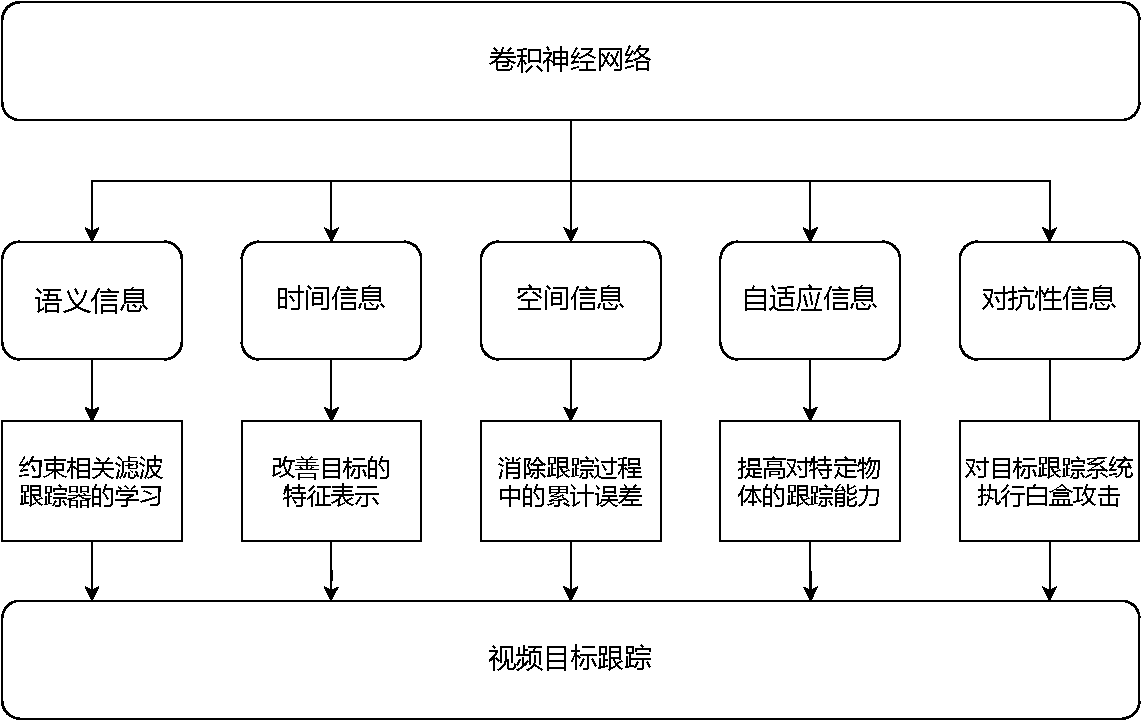
\includegraphics[width=0.75\textwidth]{Img/paper_arch.pdf}
\caption{文章组织架构}
\end{figure}

\begin{itemize}
\item{我们利用卷积神经网络获得目标的\textbf{语义信息}用于约束跟踪器的训练过程,从而提高跟踪的效果。具体而言,首先:我们提出了实例引导的相关滤波器。利用神经网络学习图像的实例级别的语义分割模板约束相关滤波器的学习。其次,针对离线训练的语义分割结果和在线学习的相关滤波结果具有互补性这一特点,我们提出了跟踪结果的自纠正机制,利用分割结果纠正相关滤波结果。我们在多个具有挑战性的视频目标跟踪数据库上验证了这些创新点在视频目标跟踪应用中的有效性。}
\item{现在的算法引入了更丰富的\textbf{空间信息}。前人工作:在空间上是局部搜索的。具体而言,我们改成了全局搜索。目的:减少累积误差并提高鲁棒性。}
\item{我们引入了\textbf{时间信息},使得目标表观特征更加丰富,从而提高跟踪的效果。}
\item{我们引入了\textbf{自适应信息}。前人工作:离线训练。目的:提高了算法对特定物体的自适应能力。}
\item{我们引入了\textbf{对抗信息},提出了一种对抗攻击算法,目的:以证明现有跟踪器的鲁棒性不太行。}
\end{itemize}

基于上述方法和创新,我们的跟踪算法在多个公开数据集上都取得了当时最好或者领先的评测结果。

\keywords{视频目标跟踪,卷积神经网络}% 中文关键词
%-
%-> 英文摘要
%-
\intobmk\chapter*{Abstract}% 显示在书签但不显示在目录

This paper is a help documentation for the \LaTeX{} class ucasthesis, which is  a thesis template for the University of Chinese Academy of Sciences. The main content is about how to use the ucasthesis, as well as how to write thesis efficiently by using \LaTeX{}.

\KEYWORDS{University of Chinese Academy of Sciences (UCAS), Thesis, \LaTeX{} Template}% 英文关键词
%---------------------------------------------------------------------------%
% title page, abstract
{% content list region
\linespread{1.2}% local line space
\intobmk*{\cleardoublepage}{\contentsname}% add link to bookmark
\tableofcontents% content catalog
\intobmk*{\cleardoublepage}{\listfigurename}% add link to bookmark
\listoffigures% figure catalog
\intobmk*{\cleardoublepage}{\listtablename}% add link to bookmark
\listoftables% table catalog
}
%\intobmk\chapter*{符号列表}% 显示在书签但不显示在目录

\section*{字符}
\nomenclatureitem[\textbf{Unit}]{\textbf{Symbol}}{\textbf{Description}}
\nomenclatureitem[$\Unit{-}$]{$\mathbb R$}{real number}
\nomenclatureitem[$\Unit{-}$]{$I$}{image frame}
\nomenclatureitem[$\Unit{-}$]{$\textbf{z}$}{template image}
\nomenclatureitem[$\Unit{-}$]{$\textbf{x}$}{search image}

\section*{算子}
\nomenclatureitem{\textbf{Symbol}}{\textbf{Description}}
\nomenclatureitem{$\mathcal F$}{the discrete Fourier transform function}
\nomenclatureitem{$\mathcal F^{-1}$}{The inverse Fourier transform of the discrete Fourier transform}
\nomenclatureitem{$\odot$}{Hadamard product}
\nomenclatureitem{$\star$}{depth-wise correlation}
\nomenclatureitem{$\nabla$}{gradient operator}

\section*{缩写}
\nomenclatureitem{DCF}{Discriminative Correlation Filter}
\nomenclatureitem{CNN}{Convolution Neural Network}
\nomenclatureitem{SGD}{Stochastic Gradient Descent}
\nomenclatureitem{GCN}{Graph Convolutional Network}
\nomenclatureitem{RNN}{Recurrent Neural Network}
\nomenclatureitem{SNN}{Spiking Neural Network}
\nomenclatureitem{RPN}{Region Proposal Network}
\nomenclatureitem{FPN}{Feature Pyramid Network}
\nomenclatureitem{GAN}{Generative Adversarial Network}
\nomenclatureitem{IoU}{Intersection over Union}
\nomenclatureitem{FFT}{Fast Fourier Transform}
\nomenclatureitem{LSTM}{Long Short-Term Memory}
\nomenclatureitem{GPU}{Graphics Processing Unit}% symbol list, preface content
%-
%-> Mainmatter
%-
\mainmatter% initialize the environment
%---------------------------------------------------------------------------%
%->> Main content
%---------------------------------------------------------------------------%
\chapter{END-TO-END TEMPORAL FEATURE AGGREGATION FOR SIAMESE TRACKERS}\label{chap:end}

\section{Introduction}
\label{sec:intro}
Visual object tracking is the task of estimating the state of an arbitrary target in each frame of a video sequence. 
%Recently, siamese network [] is introduced into visual tracking community, which has already been applied in many applications [].
%The key idea of siamese tracking architecture is, the target and the search image share the same feature extractor, then use correlation to tell the target position.
Recently, siamese networks have demonstrated the significant improvement on object tracking performances.
%However, sometimes the performance is bad 
However, the learned generic representation may be less discriminative because of the deteriorated object appearances in videos (Fig. \ref{fig:visulization}), such as motion blur, occlusion, \textit{etc}.
Researchers try different ways to improve the feature representation. 
For example, 
%RASNet \cite{wang2018learning} explores diverse attention mechanisms to adapt the offline learned feature representations to a specific tracking target.
SA-Siam \cite{he2018twofold} separately trains two branches to keep the heterogeneity of semantic/appearance features.
In DaSiamRPN \cite{zhu2018distractor}, a novel distractor-aware incremental learning module is designed, which can effectively transfer the general embedding to the current video domain and incrementally catch the target appearance variations  during inference.
SiamRPN++ \cite{li2019siamrpn++} introduces a simple yet effective sampling strategy to drive the siamese tracker with more powerful deep architectures.
These efforts have produced some impact and improved state-of-the-art accuracy.
%These improvements are useful.
%However, all these effort ignores a important problem: they ignore to merge the inter-frame feature during the training phase.
%One important solution is use the temporal information.
%The use of temporal information is important because, when one frame is bad, the adjusting frame can be used. While several method trying to use the temporal information, the method is naive.
%(The bug is, I cannot find any temporal information used in siamese trackers. (I cannot believe it!!! Check it again.--Checked)) For example, A use a time memory to store the appearance information. B use a simple feature average during test. C use history positional information to predict the object position in current frame. However, all these method cannot handle the temporal information during training, which lead to sub-optimal result. To solve this problem, 
However, all above siamese algorithms perform tracking based on features cropped from only the current frame, which limits the power of siamese trackers.

\begin{figure}[t]
    \centering
    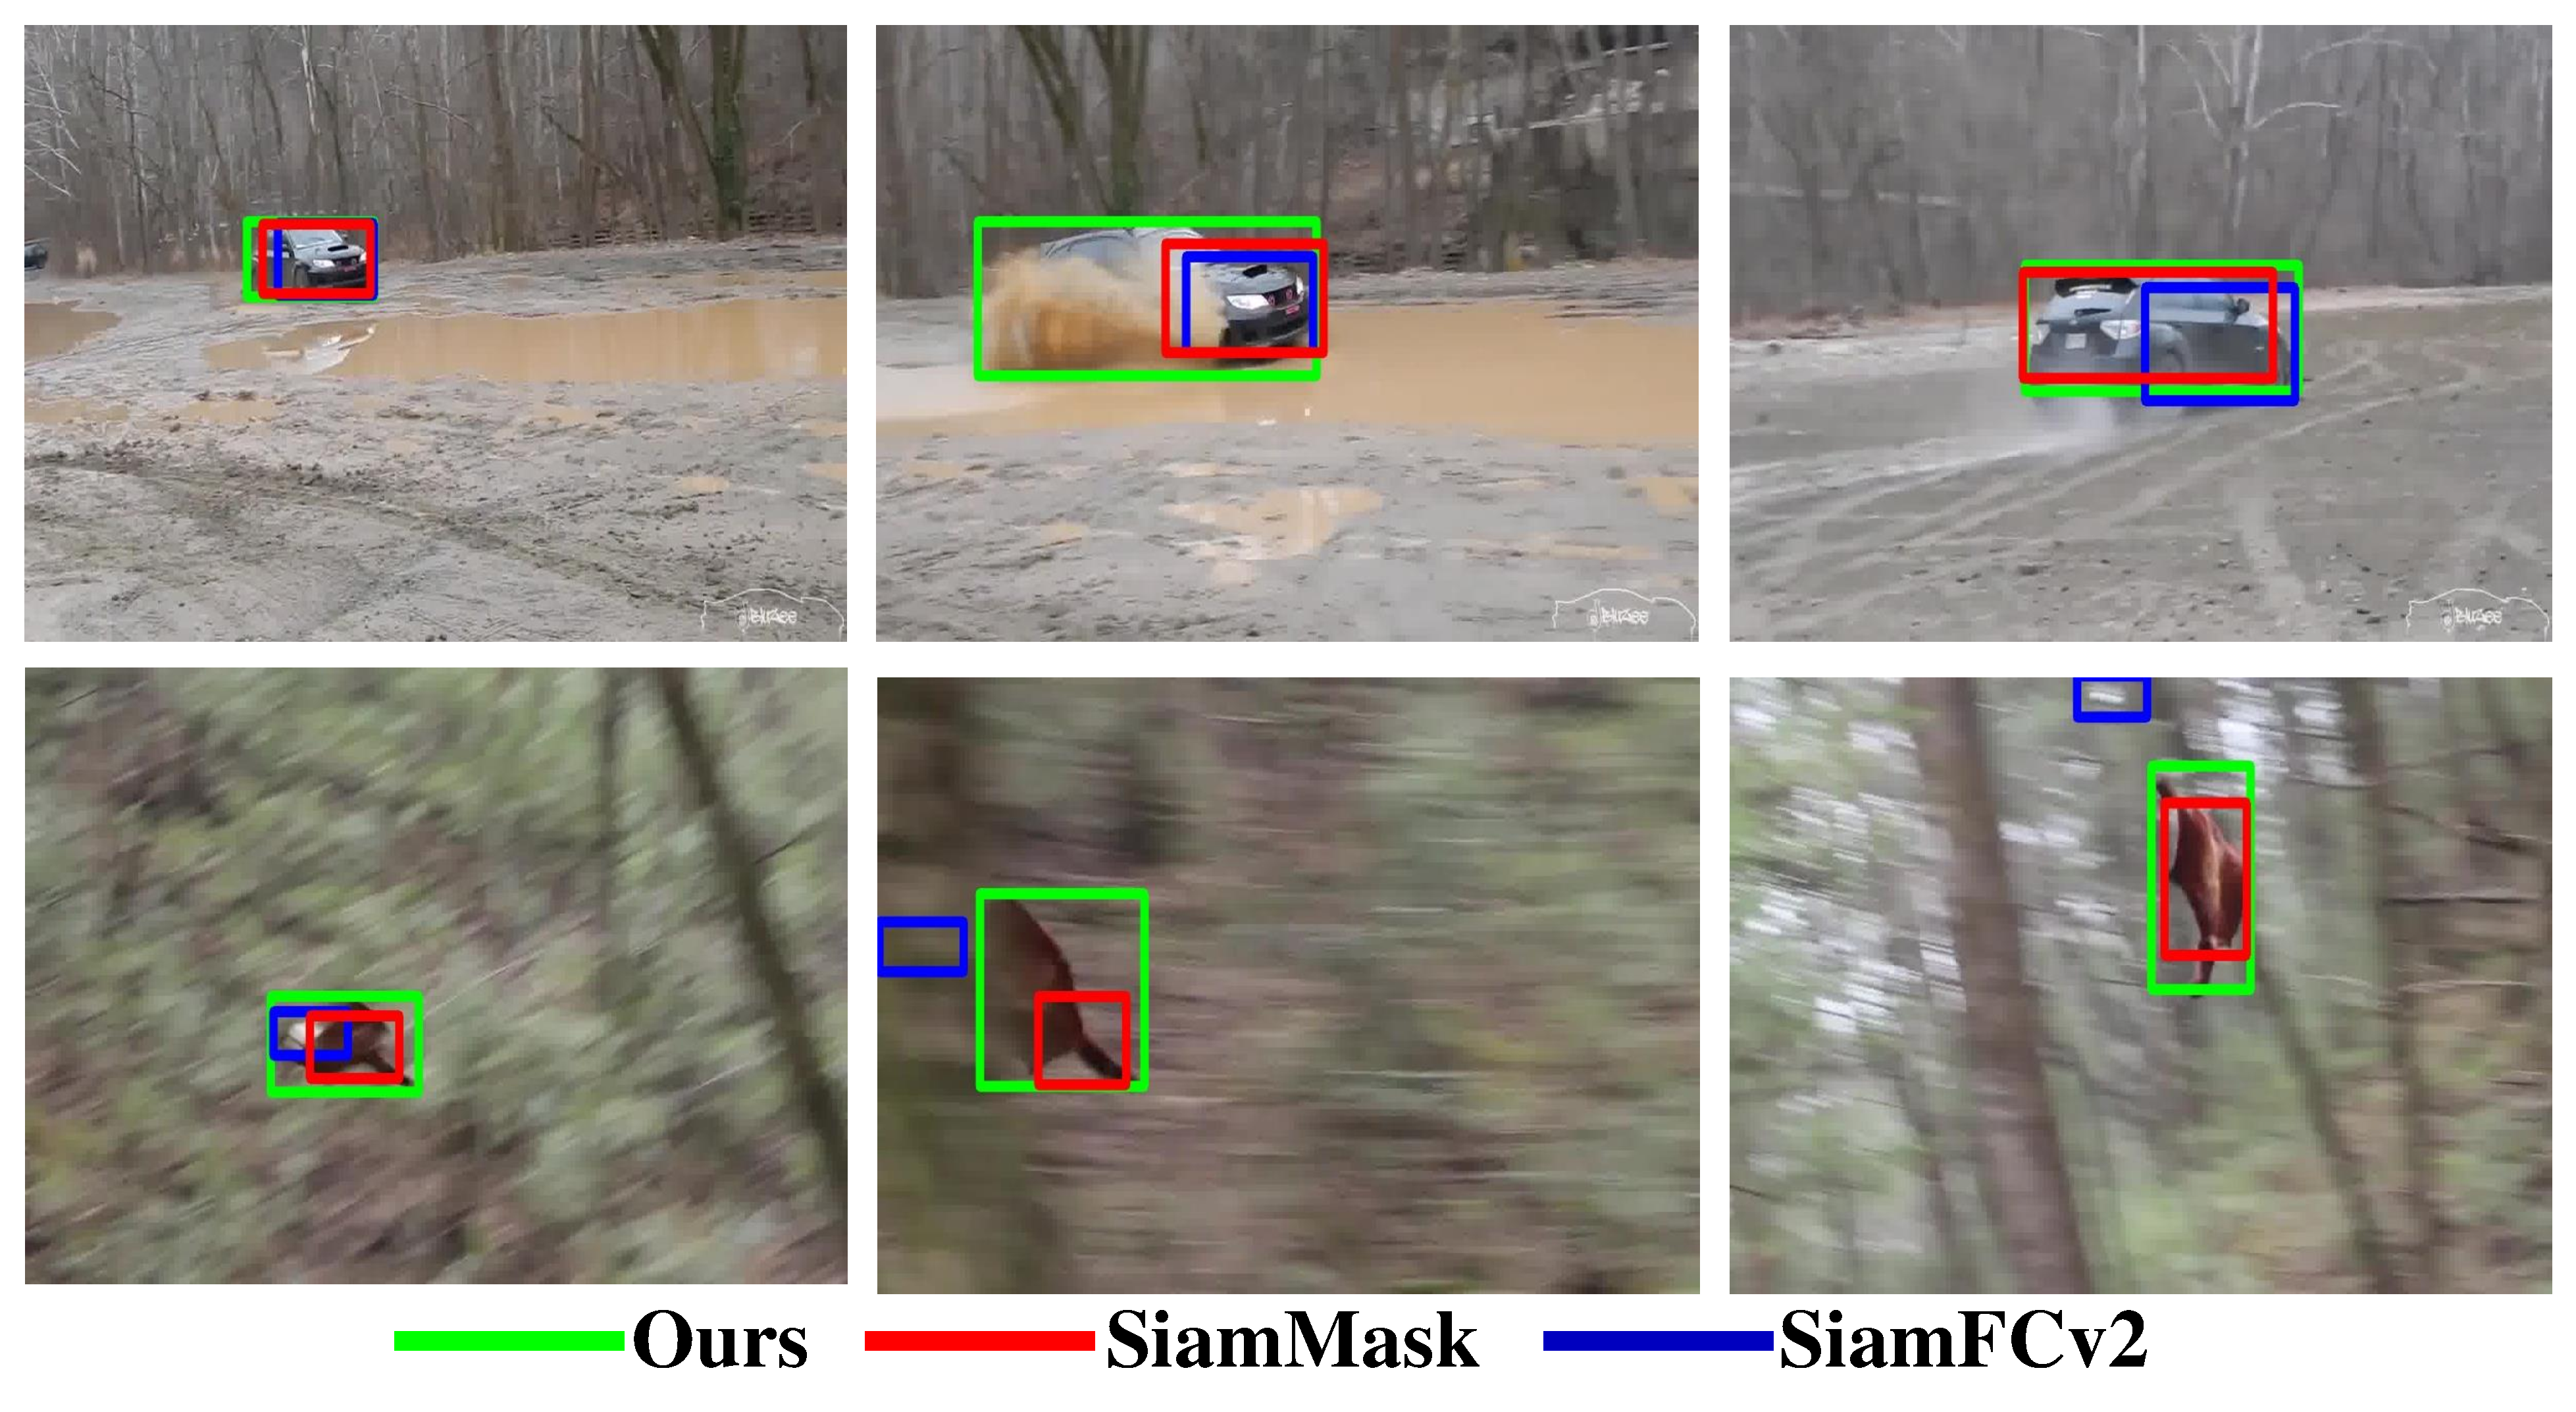
\includegraphics[width=0.48\textwidth]{Img/end/visulization.pdf}
    \vspace{-0.8cm}
    \caption{A comparison of our method with SiamMask and SiamFCv2. The example frames are from the GOT-10k testing set. Our approach effectively handles poor object appearance compared to existing approaches.}
    \vspace{-0.5cm}
    \label{fig:visulization}
\end{figure}

Actually, the video has rich information about the target and such temporal information is an important basis for video understanding and tracking.
For example, in video object detection, FGFA \cite{zhu2017flow} leverages temporal coherence on feature level. It improves the per-frame features by aggregation of nearby features along the motion paths, and thus improves the video recognition accuracy.
In video object segmentation, STCNN \cite{xu2019spatiotemporal} introduces a temporal coherence module, which focuses on capturing the dynamic appearance and motion cues to provide the guidance of object segmentation.
In discriminative correlation filter-based object tracking, FlowTrack \cite{zhu2018end} focuses on making use of the rich flow information in consecutive frames to improve the feature representation and the tracking accuracy. 
However, how to utilize the temporal information in siamese trackers has not been widely studied yet. 

\begin{figure*}[t]
    \centering
    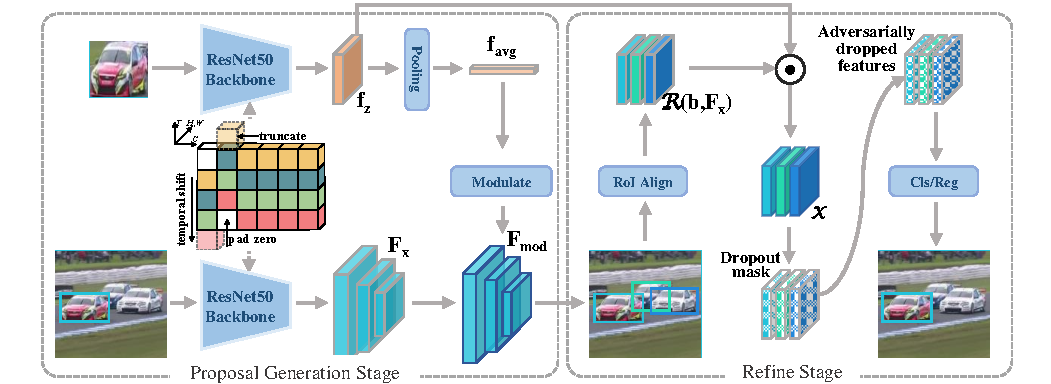
\includegraphics[width=0.9\textwidth]{Img/end/net_v3.pdf}
    \vspace{-0.5cm}
    \caption{
    Overview of our two-stage SiamTFA.
    %At the first stage, a siamese FPN equipped with a temporal aggregation module provides features of the template image and the search image. Then the feature modulation module is used to merge the features and generate proposals.
    %proposals of the object given in the first-frame bounding box. 
    %At the second stage, 
    The proposal generation stage aims to generate proposals that are visually similar to the given template target. The refine stage aims to select the target from candidate proposals.}
    \label{fig:SiamTFA}
\end{figure*}

% key words: temporal modeling, model the temporal information, temporal fusion, inter-frame information, improve the feature representation, temporal aggregation, poor object appearance
In this paper, we aim to take full advantage of temporal information in siamese trackers.
%(We introduce a novel siamese tracking architecture equipped with a temporal aggregation module to make full use of inter-frame information.)
%(In this work, to deal with the issues raised above, we propose a novel tracker to aggregate features of adjacent frames by ...)
%(In this paper, we develop an end-to-end temporal aggregation module in siamese architecture to utilize both the power of siamese trackers and the inter-frame information.)
We introduce a novel siamese tracking architecture equipped with a temporal aggregation module, which improves the per-frame features by aggregating features from adjacent frames.
This temporal fusion strategy enables the siamese tracker to handle poor object appearance like motion blur, occlusion, \textit{etc}.
To achieve this, we shift the channels along the temporal dimension \cite{lin2019tsm} in the backbone of the siamese network.
Note that features of the same object are usually not spatially aligned across frames due to video motion \cite{zhu2017flow}, so the temporal shift is only performed on the residual layers \cite{lin2019tsm} to preserve the spatial feature learning capability of the siamese tracker.
Different from other temporal fusion methods \cite{tao2016siamese, gladh2016deep}, the proposed method is able to be trained end-to-end on large-scale datasets.
%The proposed temporal aggregation module is trained end-to-end in the siamese network.
%(This module enables our module to be trained end-to-end on large-scale datasets.)
Additionally, our temporal fusion method is easy to implement, without changing the siamese tracking architecture or using optical flow \cite{zhu2018end}.

%improve the generalization ability on bad object.
%Our insight is that, if we only rely on the traditional training method, the bad image in the training data will be over wheeled by the easy cases. So the tracker shows bad performance when meeting with bad image during testing. To solve this problem, we take advantage of the recent progress in adversarial learning to increase the robustness of object features.
%Our method employs adversarial dropout to increase the robustness of object features. 
%注意,由于该模块在文章中占据次要位置,所以不应该写目前方法存在的缺点,而应该直接写用了这个模块后起到的作用。
%感觉概括性的优点不太好想,所以可以多些几句实现细节。这就要求我们弄懂代码原理。
To improve the robustness of target features, we further incorporate an adversarial dropout \cite{park2018adversarial} module in the siamese tracking network.
% add adversarial dropout to enforce the tracker to learn difficult cases. 
% (We further propose a adversarial training module to enforce the tracker to learn difficult cases. The motivation is that ... This is achieved by computing the adversarial masks based on diversity maximum. This simple form of feature selection improves the discrimination power of the tracker.)
%Specifically, we calculate the diversity of two dropouts, and make the loss max to learn the difficult dropout mask.
Specifically, we first predict adversarial dropout masks based on divergence maximum.
Then, we aim to minimize the divergence between the randomly dropped features and the adversarially dropped features.
%The effect of this module can be interpreted from both the dropout and from the adversarial training perspectives.
This module has both the advantages of dropout and adversarial training: the dropout makes our siamese network randomly disconnects neural units during training to prevent the co-adaptation of target features and the adversarial training enforces our tracker to learn difficult cases.

\iffalse
Our contributions are three folds:
(1) We introduce a novel siamese tracking architecture equipped with a temporal aggregation module, which improves the per-frame features by aggregating features of adjacent frames.
(2) We incorporate the adversarial dropout module in our tracker to improve the discrimination power of the siamese tracking network.
(3) Experiments on GOT-10k and UAV20L tracking datasets show that the proposed method performs favorably against existing state-of-the-art methods (Fig. \ref{fig:visulization}).
\fi
\iffalse
\begin{itemize}
    \item We introduce a novel siamese tracking architecture equipped with a temporal aggregation module, which improves the per-frame features by aggregating features of adjacent frames.
    \item We utilize the adversarial dropout module to improve the discrimination power of the siamese tracking network.
    \item Experiments on GOT-10k and UAV20L tracking datasets show that the proposed method performs favorably against existing state-of-the-art methods.
\end{itemize}
\fi

\section{The proposed Method}
\label{sec:method}
%应该提及我们的跟踪器的损失函数包括:对抗性损失,加上常规跟踪损失。
%In this section, we will introduce the proposed tracking method, SiamTFA (Fig. \ref{fig:SiamTFA}). 
%The main feature is:
%(1) A strong backbone. Use FPN and new-proposed feature modulation.
%(2) Equipped with 2 useful module: temporal aggregation module and adversarial dropout module to improve the robustness of features.
%In the following, three sub-section will be introduced: (1) Overview of tracking (2) Temporal aggregation module (3) Adversarial dropout module.
%网络结构怎么描述?可以参考ATOM。
%Our SiamTFA bases on a strong feature extractor -- FPN.
%We insert our temporal aggregation module in the backbone. Details of this module will be introduced at sec 3.2.
%Be robust to object size.
%FPN: handle different object size.
%modulator vector: handle different template object size.
%xcorr depth-wise: stage1 merge.
%element wise product: stage2 merge
% 介绍输入
%The input of the network is ... We use notations ... to denote ..., respectively. ... has a size of ...
%SiamTFA is composed of ... and ...
%Inspired by the great success of siamese trackers \cite{li2019siamrpn++, wang2019fast}, we also construct our SiamTFA based on the siamese architecture.
In this section, we will introduce the proposed siamese architecture-based tracking method, namely SiamTFA (Fig. \ref{fig:SiamTFA}), which is inspired by the great success of siamese trackers \cite{li2019siamrpn++, wang2019fast}.
Specifically, SiamTFA takes an image pair as input, comprising a template image and a search image. The template image is the image patch cropped from the initial frame according to ground truth bounding box. The search image is one whole frame in the remaining of the video. Both inputs share the same feature extractor and parameters.
Inspired by the success of the two stage detection paradigm \cite{ren2015faster}, our siamese tracker is also a two stage method. The first stage aims to generate proposals that are visually similar to the given template target. In this stage, we introduce a temporal aggregation module
%(Fig. \ref{fig:TSM}) 
to enhance the temporal information (Sec. \ref{sec:stage1}). The second stage aims to
identify the target from candidate proposals.
% select the target from candidate proposals. 
In this stage, we insert an adversarial dropout module to learn more robust features (Sec. \ref{sec:stage2}).

\subsection{Temporal aggregation module}
\label{sec:stage1}
% Note that 'stage1' and 'stage2' is a local term. You should introduce the global architecture which includes 'stage1' and 'stage2' first.
% You need to say something about ‘siamese' and the 'input'.
The proposal generation stage consists of 3 components: (1) feature extractor, (2) temporal aggregation module, and (3) feature modulation module.
% 需要综述三个模块在stage1中的作用。
The feature extractor generates the search features and the template feature for the search image and the template image, respectively. The temporal aggregation module is integrated into the feature extractor to utilize the temporal information. The feature modulation module merge the search features and the template feature to recognize the candidate targets.

\textbf{Feature extractor} To deal with the scale change of the target, we use Res50-FPN \cite{lin2017feature} as our feature extractor.
% You need to describe FPN here. What is FPN?
\textbf{F}eature \textbf{P}yramid \textbf{N}etwork (FPN) exploits the inherent multi-scale,  pyramidal hierarchy of deep convolutional networks to construct feature pyramids with marginal extra cost. 
Our siamese FPN takes a template image and a search image as input. For the search image, the FPN outputs proportionally sized feature maps at multiple levels, in a fully convolutional fashion.
%The input of the feature extractor is an image pair consists of a template image and a search image. The search image is resized to min size 800. The template is cropped according to ground truth bounding box and resized into 400*400. According to the siamese architecture, the template/search image share the same parameters. 
%For the search image, we got 5 different features and they have strides of \{4, 8, 16, 32, 64\} pixels with respect to the input image. For template branch, we use the last layer of FPN with size 7*7. 
We denote the output for the search image as $F_{x} = \{f_{x}^i\}_{i=1:5}$, and note that they have strides of \{4, 8, 16, 32, 64\} pixels with respect to the input search image.
For the template image, we use the last stage of the FPN output as the template feature with a spatial size of $7 \times 7$.
%Different from traditional trackers, our template/search features have temporal information. The reason is because we insert the temporal shift module into the backbone, which will be introduced next.

\textbf{Temporal aggregation module}
%Different from traditional trackers, we use the rich information about the same object instance by 
Most popular siamese trackers \cite{li2019siamrpn++, wang2019fast} use the still image to make prediction. % However, tracking on single frame generates unstable results and fails when appearance is pool \cite{zhu2017flow}. 
This limits the ability of these siamese trackers.
On one hand, tracking on single frame generates unstable results and fails when appearance is poor (Fig. \ref{fig:visulization}); on the other hand, 
temporal adjacent frames can provide more information about the target.
%the video has rich information about the target. 
So we aim to improve the per-frame features by aggregating features of adjacent frames.
Specifically, we insert a temporal aggregation module into the last stage of the feature extractor. 
% We have to cite TSM, because we use this idea.
To model temporal information, the images in one batch are several adjacent frames in the same video and are sorted by time, so we can regard the batch dimension as the time dimension. Assume the feature map at the last stage of the feature extractor is $f \in \mathbb R ^ {T \times C \times H \times W}$.
For each time $t \leq T$, we first split feature $f^t \in \mathbb R ^ {C \times H \times W}$ into 3 parts along the channel dimension: $f_{1:K}^t \in \mathbb R ^ {K \times H \times W}$, $f_{(K+1):2K}^t \in \mathbb R ^ {K \times H \times W}$, and $f_{(2K+1):C}^t \in \mathbb R ^ {(C-2K) \times H \times W}$.
Then we shifts the channels along the temporal dimension following \cite{lin2019tsm}:
% Then The aggregated function at time $t$ is:
\begin{equation}
    f_{agg}^t = \mathcal{C}(f_{{1:K}}^{t-1}, f_{(K+1):2K}^{t+1}, f_{(2K+1):C}^{t}),
\end{equation}
where $\mathcal{C}(\cdot)$ is the concatenation operation. According to \cite{lin2019tsm}, the shift operation is only performed at the residual layer to preserve the spatial feature learning capability of the siamese tracker.
Note that the aggregated feature $f_{agg}^t$ has the same shape with $f^t$, so we can insert this module into the backbone directly, without the need to change other part of the network.
What's more, this operation only needs to do data movement, so it is computationally free and can be trained end-to-end.
% Say the effect of this module.
%After performing such channel fusion, rich target information in adjacent frames can be aggregated into the current frame. For example, if the current frame is blurred, target information that is not blurred in adjacent frames can be used.

\iffalse
\begin{figure}[t]
    \centering
    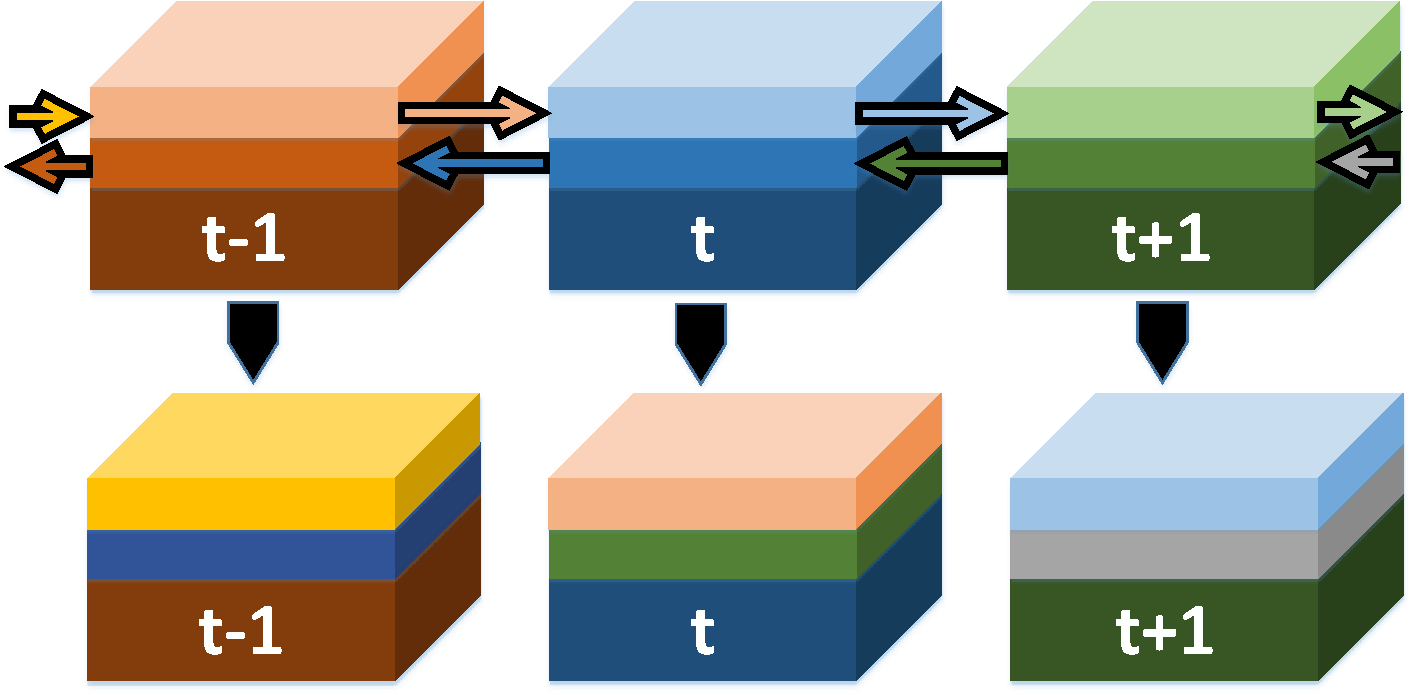
\includegraphics[width=0.4\textwidth]{images/TSM_v1.pdf}
    \caption{Temporal aggregation module.}
    \label{fig:TSM}
\end{figure}
\fi

\textbf{Feature modulation module} After getting the template feature $f_{z}$ and the search feature pyramid $F_{x} = \{f_{x}^i\}_{i=1:5}$, they are modulated to generate target-specific features.
Specifically, The modulation vector $f_{avg}$ is generated from $f_{z}$ using global average pooling, which carries the target-specific appearance information. 
%The search feature pyramid is $F = \{f_1, f_2, f_3\}$. 
%For $f_{x}^{i} \in F_{x}$, t
The modulated feature pyramid $F_{mod} = \{f_{mod}^i\}_{i=1:5}$ is generated as follows:
\begin{equation}
    f_{mod}^i = \mathcal{M}(f_{avg}, f^i_x),
\end{equation}
where $\mathcal M(\cdot)$ is the depth-wise correlation \cite{li2019siamrpn++}.
%So we get the modulated feature pyramid $F_{mod} = \{f_{mod}^i\}_{i=1:5}$. 
%Then we predict proposals on $F_{mod}$.
Each modulated feature map is fed into two sibling fully-connected layers---a box-regression layer with channel dimension 4$k$, and a box classification layer with channel dimension 2$k$, where $k$ is the number of maximum possible proposals for each location.
% anchor 这个概念是必备的,所以是得讲一下。
The object/background criterion and bounding box regression are defined with respect to a set of anchors.
Following \cite{lin2017feature}, we assign anchors with the same scale to each of the different pyramid levels. For detail information of the anchor setting, please refer to \cite{lin2017feature}.
% For every modulated layer, we attach a classification layer and a regression layer to make predict.
\iffalse
The loss function of stage 1 is:
\begin{equation}
    \mathcal{L}_1 = 
\end{equation}
\fi
% you need to say how we get the candidates. Faster R-CNN already says it.
%The generated proposes with top-K classification scores is send to stage2.
We use the top-$N$ ranked proposal regions for the refine stage.

\subsection{Adversarial dropout module}
%stage 1 的网络结构已经交代清楚了,就是一个FPN。和调制,和分类/回归层。那么stage的网络结构也应该交代清楚:roi align + 特征融合 + 对抗 + 分类/回归层。
\label{sec:stage2}
% 首先你要讲一下stage2在全局中的作用。
The refine stage aims to select the target from candidate proposals.
% 或许该讲一下stage2的输入包括:真实目标特征+候选区域。
% The input of stage 2 consists of: (1) The target feature is $f_{z} \in \mathbb R ^{256 \times 7 \times 7}$. (2) The candidate boxes generated from stage 1.
% Stage 2 compose of a feature merge module, a adversarial dropout module, a classifier layer $h^{cls}$ and a regression layer $h^{reg}$. 
Features of these candidate proposals are cropped from the search feature pyramid $F_{x}$ using RoIAlign \cite{he2017mask}, and then fused with the target feature $f_{z}$:
\begin{equation}
    \mathcal{X} = \mathcal{R}(b, F_{x}) \odot f_{z},
\end{equation}
where $\mathcal{R}$ represents the RoIAlign, $\odot$ represents the element-wise multiplication, $b$ represents an RoI in candidate proposals and $\mathcal{X}$ represents the fused feature of $b$.
%where $x' \in \mathbb R ^{256 \times 7 \times 7}$.
%$x' \in \mathbb R ^{256 \times 7 \times 7}$ is the feature of an RoI cropped from unmodulated feature pyramid using RoIAlign \cite{he2017mask}.
%The merged feature of a candidate target is:$x = x' \odot x_0$, where $\odot$ represents the element-wise multiplication. $x$ is the merged feature of that RoI.
% Maybe you need to say why you do the merge again.
% The modulation in stage 1 and the feature merge in stage 2 play different part in the tracking process. The modulation aims to detect the similar appearance in the whole image. The

\textbf{Adversarial dropout} After the feature fusion, we use adversarial dropout \cite{park2018adversarial, lee2019drop} to increase the discriminative ability of $\mathcal{X}$.
% 简短的描述你是怎么做的。这是很重要的,让读者先对你的东西有个大概的了解,才能进一步了解细节。
We first predict the adversarial dropout mask based on divergence maximum. The mask is applied to $\mathcal{X}$ to get the adversarially dropped features.
Then, we aim to minimize the divergence between the randomly dropped features and the adversarially dropped features.
%Specifically, we donate the random mask as $m^s$, the adversarial mask as $m^{adv}$.
Specifically, let $h^{cls}$ and $h^{reg}$ denote the classification layer and the regression layer in stage 2, respectively.
The adversarial dropout mask is calculated as follows according to \cite{lee2019drop}:
\begin{equation}
\begin{split}
    & \mathbf{m}^{adv} = \mathop{\arg\max}\limits_{\mathbf{m}}D[h^{cls}(\mathcal{X} \odot \mathbf{m}^s), h^{cls}(\mathcal{X} \odot \mathbf{m})] \\
    & where~||\mathbf{m}^s - \mathbf{m}|| \leq \delta_e L,
\end{split}
\end{equation}
where $L$ represents the dimension of $\mathbf{m} \in \mathbb R^L$,
$\mathbf{m}^s$ represents the random mask and $\mathbf{m}^{adv}$ represents the adversarial mask.
$\delta_{e}$ is a hyper parameter to control the perturbation magnitude with respect to $\mathbf{m}^{s}$ \cite{lee2019drop}.
%and $\delta_{e}$ is a hyper parameter to control the perturbation magnitude with respect to $m^{s}$ \cite{lee2019drop}
$D[p, p']  \geq 0$ measures the divergence between two distributions $p$ and $p'$.

To calculate $\mathbf{m}^{adv}$, \cite{park2018adversarial} optimizes a 0/1 knapsack problem with appropriate relaxations in the process. Please refer to \cite{park2018adversarial} for detail information.
%Then, we use the mask to dropout the feature, then send it to the classifier.
%We also send the clean feature to the classifier, and wish the loss minimum:
After generating $\mathbf{m}^{adv}$, we then aim to minimize the divergence between two predicted distribution regarding to $\mathcal{X}$: one with a random dropout mask $\mathbf{m}^{s}$ and another with an adversarial dropout mask $\mathbf{m}^{adv}$ \cite{lee2019drop}.
\begin{equation}
    \mathcal{L}_{adv} = \mathbb E[D_{KL}[h^{cls}(\mathcal{X} \odot\mathbf{m}^{s})||h^{cls}(\mathcal{X} \odot\mathbf{m}^{adv}))]],
\end{equation}
where $D_{KL}$ is the Kullback-Leibler divergence.

Finally, for each RoI, the classification layer produces softmax probability estimates over two classes (foreground or background) and the regression layer outputs four real-valued numbers for the foreground class. These four values encode the refined bounding-box position for the RoI.
The loss of SiamTFA is:
%The RoI Aligned features are fed into the global average pooling layer followed by two sibling output layers: one that produces softmax probability estimates over two classes (foreground or background) and another layer that outputs four real-valued numbers for the foreground class. These four values encode the refined bounding-box position for the RoI.
%We get the final tracking result as follows: The classification layer $h^{cls}$ predicts a score for a RoI, the regression layer $h^{reg}$ has shape * and predicts a 4-d vector for it.
%The RoI with the top score is the final box.
\begin{equation}
\mathcal{L} = \mathcal{L}_{cls}^{stage1} + \mathcal{L}_{cls}^{stage2} + \mathcal{L}_{reg}^{stage1}+\mathcal{L}_{reg}^{stage2} +  \lambda \mathcal{L}_{adv},
\end{equation}
where $\lambda$ is a hyper-parameter to balance the adversarial loss and the classification/regression loss. $\mathcal{L}_{cls}^{\cdot}$ is the cross entropy loss and $\mathcal{L}_{reg}^{\cdot}$ is the standard smooth $L1$ loss for regression. During testing, the RoI with the top classification score is selected as the predicted target.


\iffalse
{classification/regression} The structure of $f^{cls}$ is ... The structure of $f^{reg}$ is ...
Suppose $B^*_t$ is the target bounding box at frame $t$, which is estimated through:
\begin{equation}
B^*_t = h^{reg}(\mathop{\arg\max}\limits_{x \in \mathcal{X}}h^{cls}(x)), 
\end{equation}
where $\mathcal{B}_t^1$ is a set of proposals generated from stage 1.
\fi

\section{Experiments}
In this section, we first present the implementation details.
Then we evaluate out method on GOT-10K \cite{Huang_2019} testing set and the UAV20L \cite{mueller2016benchmark} dataset.
\vspace{-2mm}
\subsection{ Implementation details}
The proposed network is trained on the training set of GOT-10k \cite{Huang_2019} and the backbone is pretrained on ImageNet.
We apply stochastic gradient descent with momentum of 0.9 and set the weight decay to 0.0005.
The learning rate is decreased from $10^{-2}$ to $10^{-4}$.
The batch size is set to 2 and the network is trained for 90000 iterations.
Our tracker is implemented in Python, using PyTorch.
%First stage, we select 4000 proposals to send to stage2, the positive/negative rate is 1:3.
%To shift channels $K=2$.
%Because of the memory limit, the batch size is 2.
%To calculate the loss, $\lambda = 1$.
%For both training and testing, the size of a template image is 
% 其实有些对不上。按论文上讲,第一阶段是找到若干候选框。第二阶段是得到唯一结果。实际上是,第一阶段得到若干候选框,第二阶段进一步筛选得到约10个候选框(这才是真正的相似目标),然后按IoU和得分来选择最终结果。
% For test, we select top 100 proposals to send to stage2. The we use NMS to select top 10 object. 
\vspace{-2mm}
\subsection{Evaluation on GOT-10k dataset}

\iffalse
\begin{figure}[t]
    \centering
    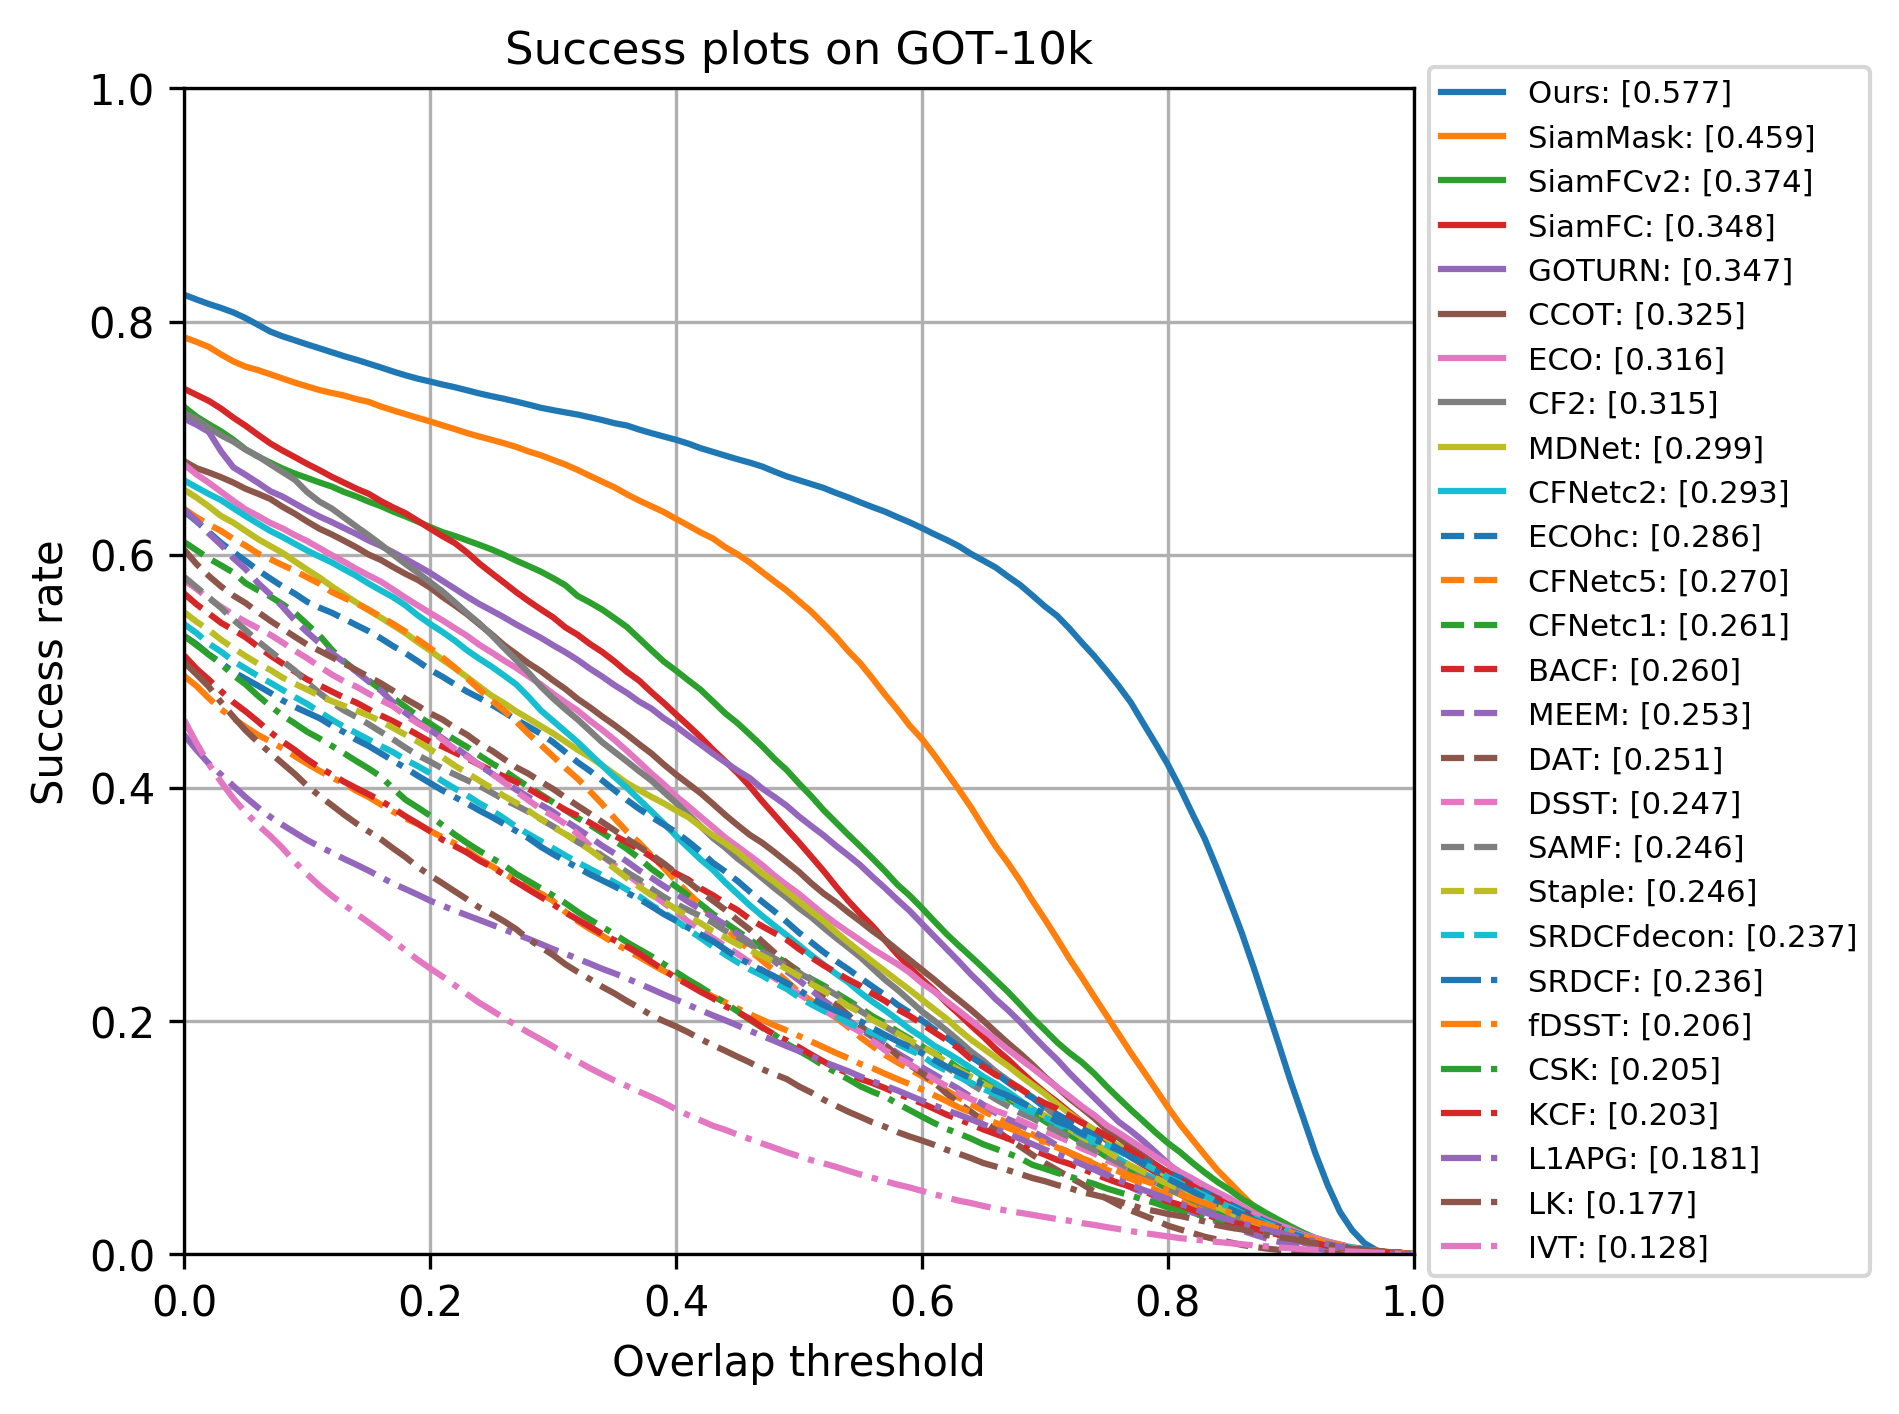
\includegraphics[width=0.45\textwidth]{images/success_plot.png}
    \vspace{-5mm}
    \caption{Overall performance on GOT-10k, ranked by their average overlap (AO) scores.}
    \label{fig:got10k}
     \vspace{-3mm}
\end{figure}
\fi
\begin{table}
\centering
\caption{Performance of our algorithm with different components on GOT-10k test set.}
\begin{tabular}{c c c c c}
\bottomrule
\begin{tabular}[x]{@{}c@{}}Temporal\\aggregation\end{tabular} & \begin{tabular}[x]{@{}c@{}}Adversarial\\dropout\end{tabular} & $AO$ & $SR_{0.50}$ & $SR_{0.75}$ \\ 
\hline
          &           & 0.542 & 0.607 & 0.456 \\
\checkmark&           & 0.561 & 0.645 & 0.480 \\
\checkmark&\checkmark & 0.577 & 0.662 & 0.509 \\
\bottomrule
\label{tabel:ablation}
\end{tabular}
\vspace{-0.8cm}
\end{table}
\begin{table}
\centering
\caption{Comparing the results of our approach against other approaches over the GOT-10k test set.}
\begin{tabular}{l l l l}
\bottomrule
Method   &  $AO$   &  $SR_{0.50}$ & $SR_{0.75}$  \\
\hline
Ours &  $\textbf{0.577}^\textbf{1}$ & $\textbf{0.662}^\textbf{1}$  & $\textbf{0.509}^\textbf{1}$  \\
SiamMask &  0.459&  0.560 &0.205 \\
SiamFCv2 &  0.374&  0.404 &0.144 \\
SiamFC   &  0.348&  0.353 &0.098 \\
GOTURN	 &  0.347&  0.375 &0.124 \\
CCOT	 &  0.325&  0.328 &0.107 \\
ECO	     &  0.316&  0.309 &0.111 \\
CF2	     &  0.315&  0.297 &0.088 \\
MDNet	 &  0.299&  0.303 &0.099 \\
%CFNetc2	 &  0.293&  0.265 &0.087 \\
%ECOhc	 &  0.286&  0.276 &0.096 \\
\bottomrule
\end{tabular}
\label{table:got}
\end{table}
In this subsection, we evaluate our method on GOT-10k \cite{Huang_2019} dataset.
% Say something about this dataset.
GOT-10k is a recent large-scale high-diversity dataset consisting of over 10,000 video sequences with targets annotated by axis-aligned bounding boxes. 
%Note that the classes between training and test sets are zero-overlapped. 
%This one-shot protocol avoids the evaluation bias towards familiar objects. 
The GOT-10k testing set includes 180 sequences with 84 different object classes and 32 motion patterns. As performance measure, we use the average overlap (AO) scores and success rate (SR) as proposed in \cite{Huang_2019}. The AO denotes the average of overlaps between all groundtruth and estimated bounding boxes, while the SR measures the percentage of successfully tracked frames where the overlaps exceed 0.5/0.75.

\textbf{Ablation Studies}
From Table \ref{tabel:ablation} (the $1^{st}$ and $2^{nd}$ row), we see that the AO performance increases by 1.9\% by adding the temporal aggregation module.
This is because the temporal aggregation module improves the per-frame features by aggregating temporal information from adjacent frames.
%The RPN stage rapidly filters out most background samples, and the RoI head adopts a fixed foreground-to-background ratio to maintain a manageable balance between foreground and background.
From Table \ref{tabel:ablation} (the $2^{nd}$ and $3^{rd}$ row), we see that with the adversarial dropout module, the AO increases by 1.6\%.
%This is because the proposed motion model can effectively predict the position distribution of the target, effectively avoiding the adverse effects of distractors. 
This is because the adversarial dropout module improves the discrimination power of our siamese tracking network.

\textbf{Overall Performance}
We compare our proposed method with 8 trackers, including state-of-the-arts.
The performances of the evaluated trackers is shown in Table \ref{table:got}.
Compared to other listed approaches, our approach achieves a superior AO of 0.577.
%ECO \cite{danelljan2017eco} is a state-of-the-art DCF-based tracker, which introduces a factorized convolution operator that dramatically reduces the number of parameters in the DCF model. In contrast, our tracker is based on the powerful siamese architecture. As a result, our tracker significantly outperforms ECO with a gain of 26.1\% in terms of AO score, which suggests the effectiveness of the siamese architecture for the object tracking task.
%SiamMask \cite{wang2019fast} is a recently proposed siamese tracker. It simultaneously trains a siamese network on three tasks, each corresponding to a different strategy to establish correspondences between the target object and candidate regions in the new frames.
% However, it is based on the local search mechanism: searching the target within a small neighborhood centered on the target position of the previous frame. In the contrast, our SiamTFA use the the global search mechanism. It is always able to perceive the target over the entire image. As a result, our tracker outperforms SiamMask by relative * in terms of AO, which highlights ...
Compared with SiamMask, our tracker aims to make full use of the temporal information. As a result, our tracker outperforms SiamMask by 11.8\% in terms of AO, which highlights the importance of the proposed temporal aggregation module.

\begin{figure}[t]
\begin{minipage}[b]{.48\linewidth}
  \centering
  \centerline{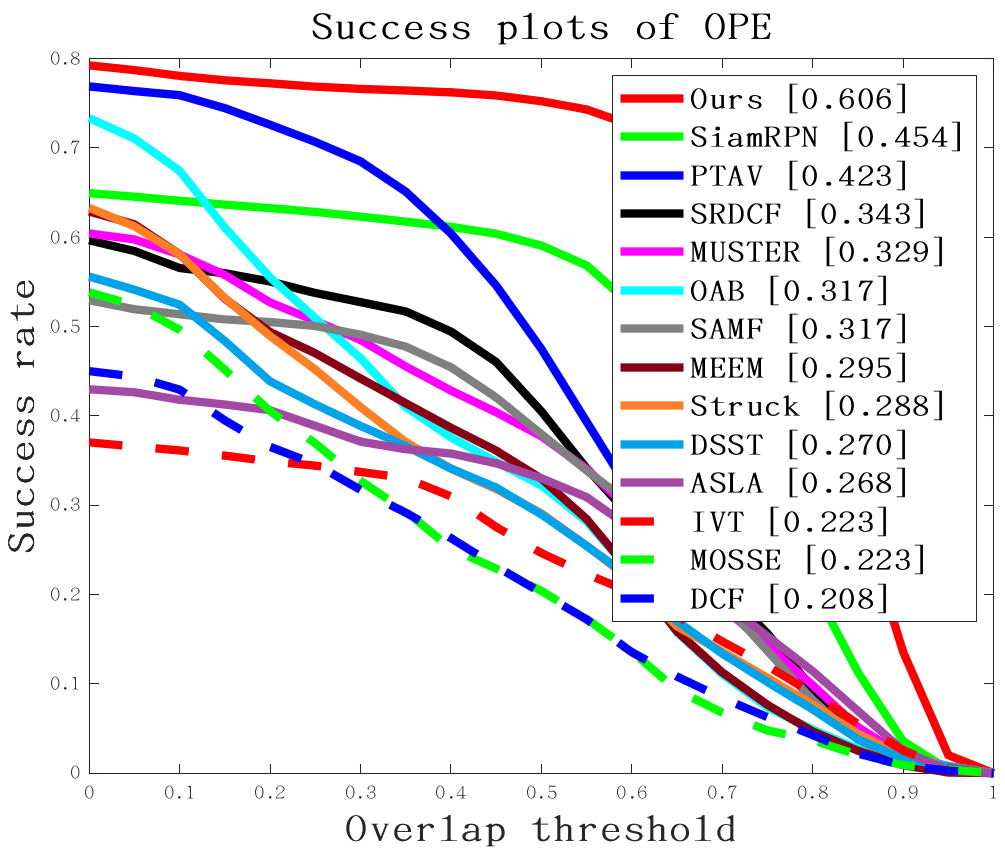
\includegraphics[width=5.0cm]{Img/end/quality_plot_overlap_OPE_AUC.png}}
\end{minipage}
\hfill
\begin{minipage}[b]{0.48\linewidth}
  \centering
  \centerline{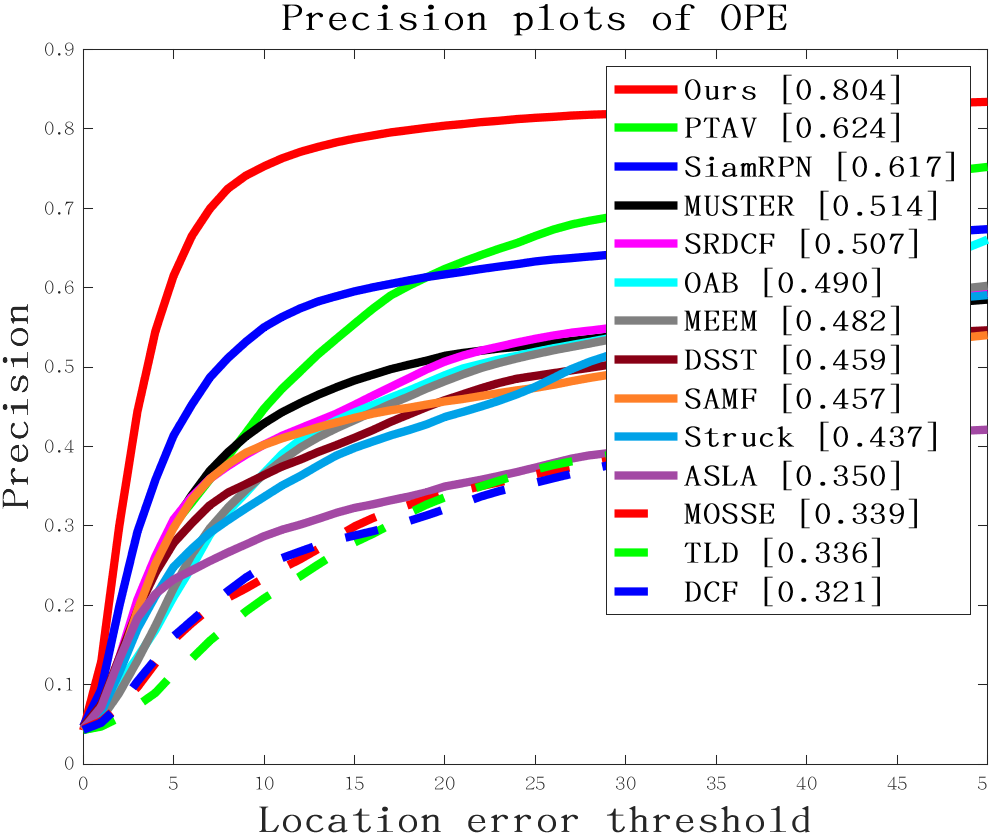
\includegraphics[width=5.0cm]{Img/end/quality_plot_error_OPE_threshold.png}}
\end{minipage}
\vspace{-5mm}
%
\caption{Success and precision plots on UAV20L dataset.}
\vspace{-3mm}
\label{fig:uav20l}
%
\end{figure}
\vspace{-2mm}
\subsection{Evaluation on UAV20L dataset}
In this subsection, we evaluate our tracker on the UAV20L \cite{mueller2016benchmark} long term tracking dataset.
% say something about this dataset: length, 20段
It contains 20 HD video sequences captured from a low-altitude aerial perspective with average sequence length of 2934 frames.
% It has mean frames of 2934 and max frames of 5527.
% say something about the measures. 
In this experiment, all trackers are compared using two measures: precision and success. Precision is measured as the distance between the centers of the predicted bounding box and the corresponding ground truth bounding box. Success is measured as the intersection over union of pixels in predicted bounding box and those in ground truth bounding box.
% say something about the accuracy.
In Fig. \ref{fig:uav20l}, we can find that the proposed algorithm achieves better tracking performance compared with some representative trackers.
In the success plot, our tracker obtains an AUC score of 0.606.
% PTAV is ... Compared with it, our is higher. This demonstrates the effectiveness of our designed architecture.
In the precision plot, the proposed algorithm obtains a score of 0.804.
% MUSTER is ... Compared with it, our is higher.
It shows that our tracker surpass other state-of-the-art algorithms, such as SiamRPN \cite{li2018high} and PTAV \cite{fan2017parallel}. This demonstrates the effectiveness of our tracker in long-term tracking scenario. 
%designed architecture.
%It shows that our tracker surpass another siamese tracker -- SiamRPN. This demonstrates the effectiveness of our designed architecture. Moreover, compared with other state-of-the-art algorithms, such as PTAV \cite{} and MUSTER \cite{}, our trackers are still superior in terms of precision.
\section{Conclusion}
%一句话指出我们提出了什么。
In this paper, we introduce a novel siamese architecture for visual object tracking.
Specifically, our proposed algorithm contains two main modules, \textit{i.e.} temporal aggregation module and adversarial dropout module. The temporal aggregation module improves  the per-frame features by aggregating features of adjacent frames. The adversarial dropout module improves the discrimination power of the siamese tracking network.
%say something about the experiment.
Extensive experimental results show that the proposed algorithm performs favorably against the state-of-the-art algorithms.
\chapter{自适应信息增强的视觉目标跟踪算法研究}\label{chap:MTP}
在本章中,我们表明可以通过简单地在孪生网络中操纵模板图像的像素来处理视觉目标跟踪中具有挑战性的模型自适应任务。对于不包含在离线训练集中的目标,对模板图像像素的稍加修改即可改善离线训练的孪生网络的预测结果。流行的对抗样本生成方法可用于执行模板像素操纵以进行模型自适应。与当前的模板更新方法(旨在合并先前帧的目标特征)不同,我们专注于在第一帧中使用目标真实注释框进行初始自适应。本章提出的模型自适应方法是即插即用的,不会改变基线跟踪器的总体架构。
全面的实验证明了本章提出的自适应信息增强的视觉目标跟踪算法的有效性。
%据我们所知,这项工作是直接操纵模板像素以在基于孪生的跟踪器中进行模型调整的首次尝试。
%在最近的基准测试中进行的大量实验表明,我们的方法比其他一些最新的跟踪器具有更好的性能。
%我们的代码可从 https://github.com/lizhenbang56/MTP 获得。

\section{引言}
视觉目标跟踪是指仅在指定目标初始状态的情况下,在视频序列中定位该目标运动轨迹的任务。最近,孪生网络 \cite{danelljan2019atom, SiamFC} 已经为视觉目标跟踪的性能带来了显著提高。孪生跟踪器将视觉目标跟踪问题形式化为学习目标模板和搜索区域之间的相似性。搜索图像中与目标模板视觉相似度最高的位置被确定为目标在当前帧的位置,从而进行跟踪。尽管孪生网络跟踪器已经成为了主流的视觉目标跟踪算法,但对于不包含在离线训练集中的目标,所学习的孪生网络相似度不一定可靠,从而导致泛化效果较差 \cite{Bhat_2019_ICCV}。最近的一些工作旨在使模型适应当前目标的表观信息。例如,TADT \cite{Li_2019_CVPR} 根据反向传播的梯度识别每个卷积滤波器的重要性,并使用目标的激活来选择重要的目标特征。然而,TADT 的特征提取器是在 ImageNet \cite{VID} 上而不是在大规模视觉目标跟踪数据集上进行预训练的。这限制了其特征在目标跟踪任务上的表示能力。GradNet \cite{Li_2019_ICCV} 利用梯度中的判别性信息,通过前向传播和反向传播操作更新孪生网络中的模板。然而,该算法采用的额外子网会增加计算成本,并且容易过拟合。UpdateNet \cite{Zhang_2019_ICCV} 学习合并先前帧中的目标特征。然而,该方法不使用真实标注信息来自适应地调整第一帧的模板特征。

\iffalse
\begin{figure}[t]
    \centering
    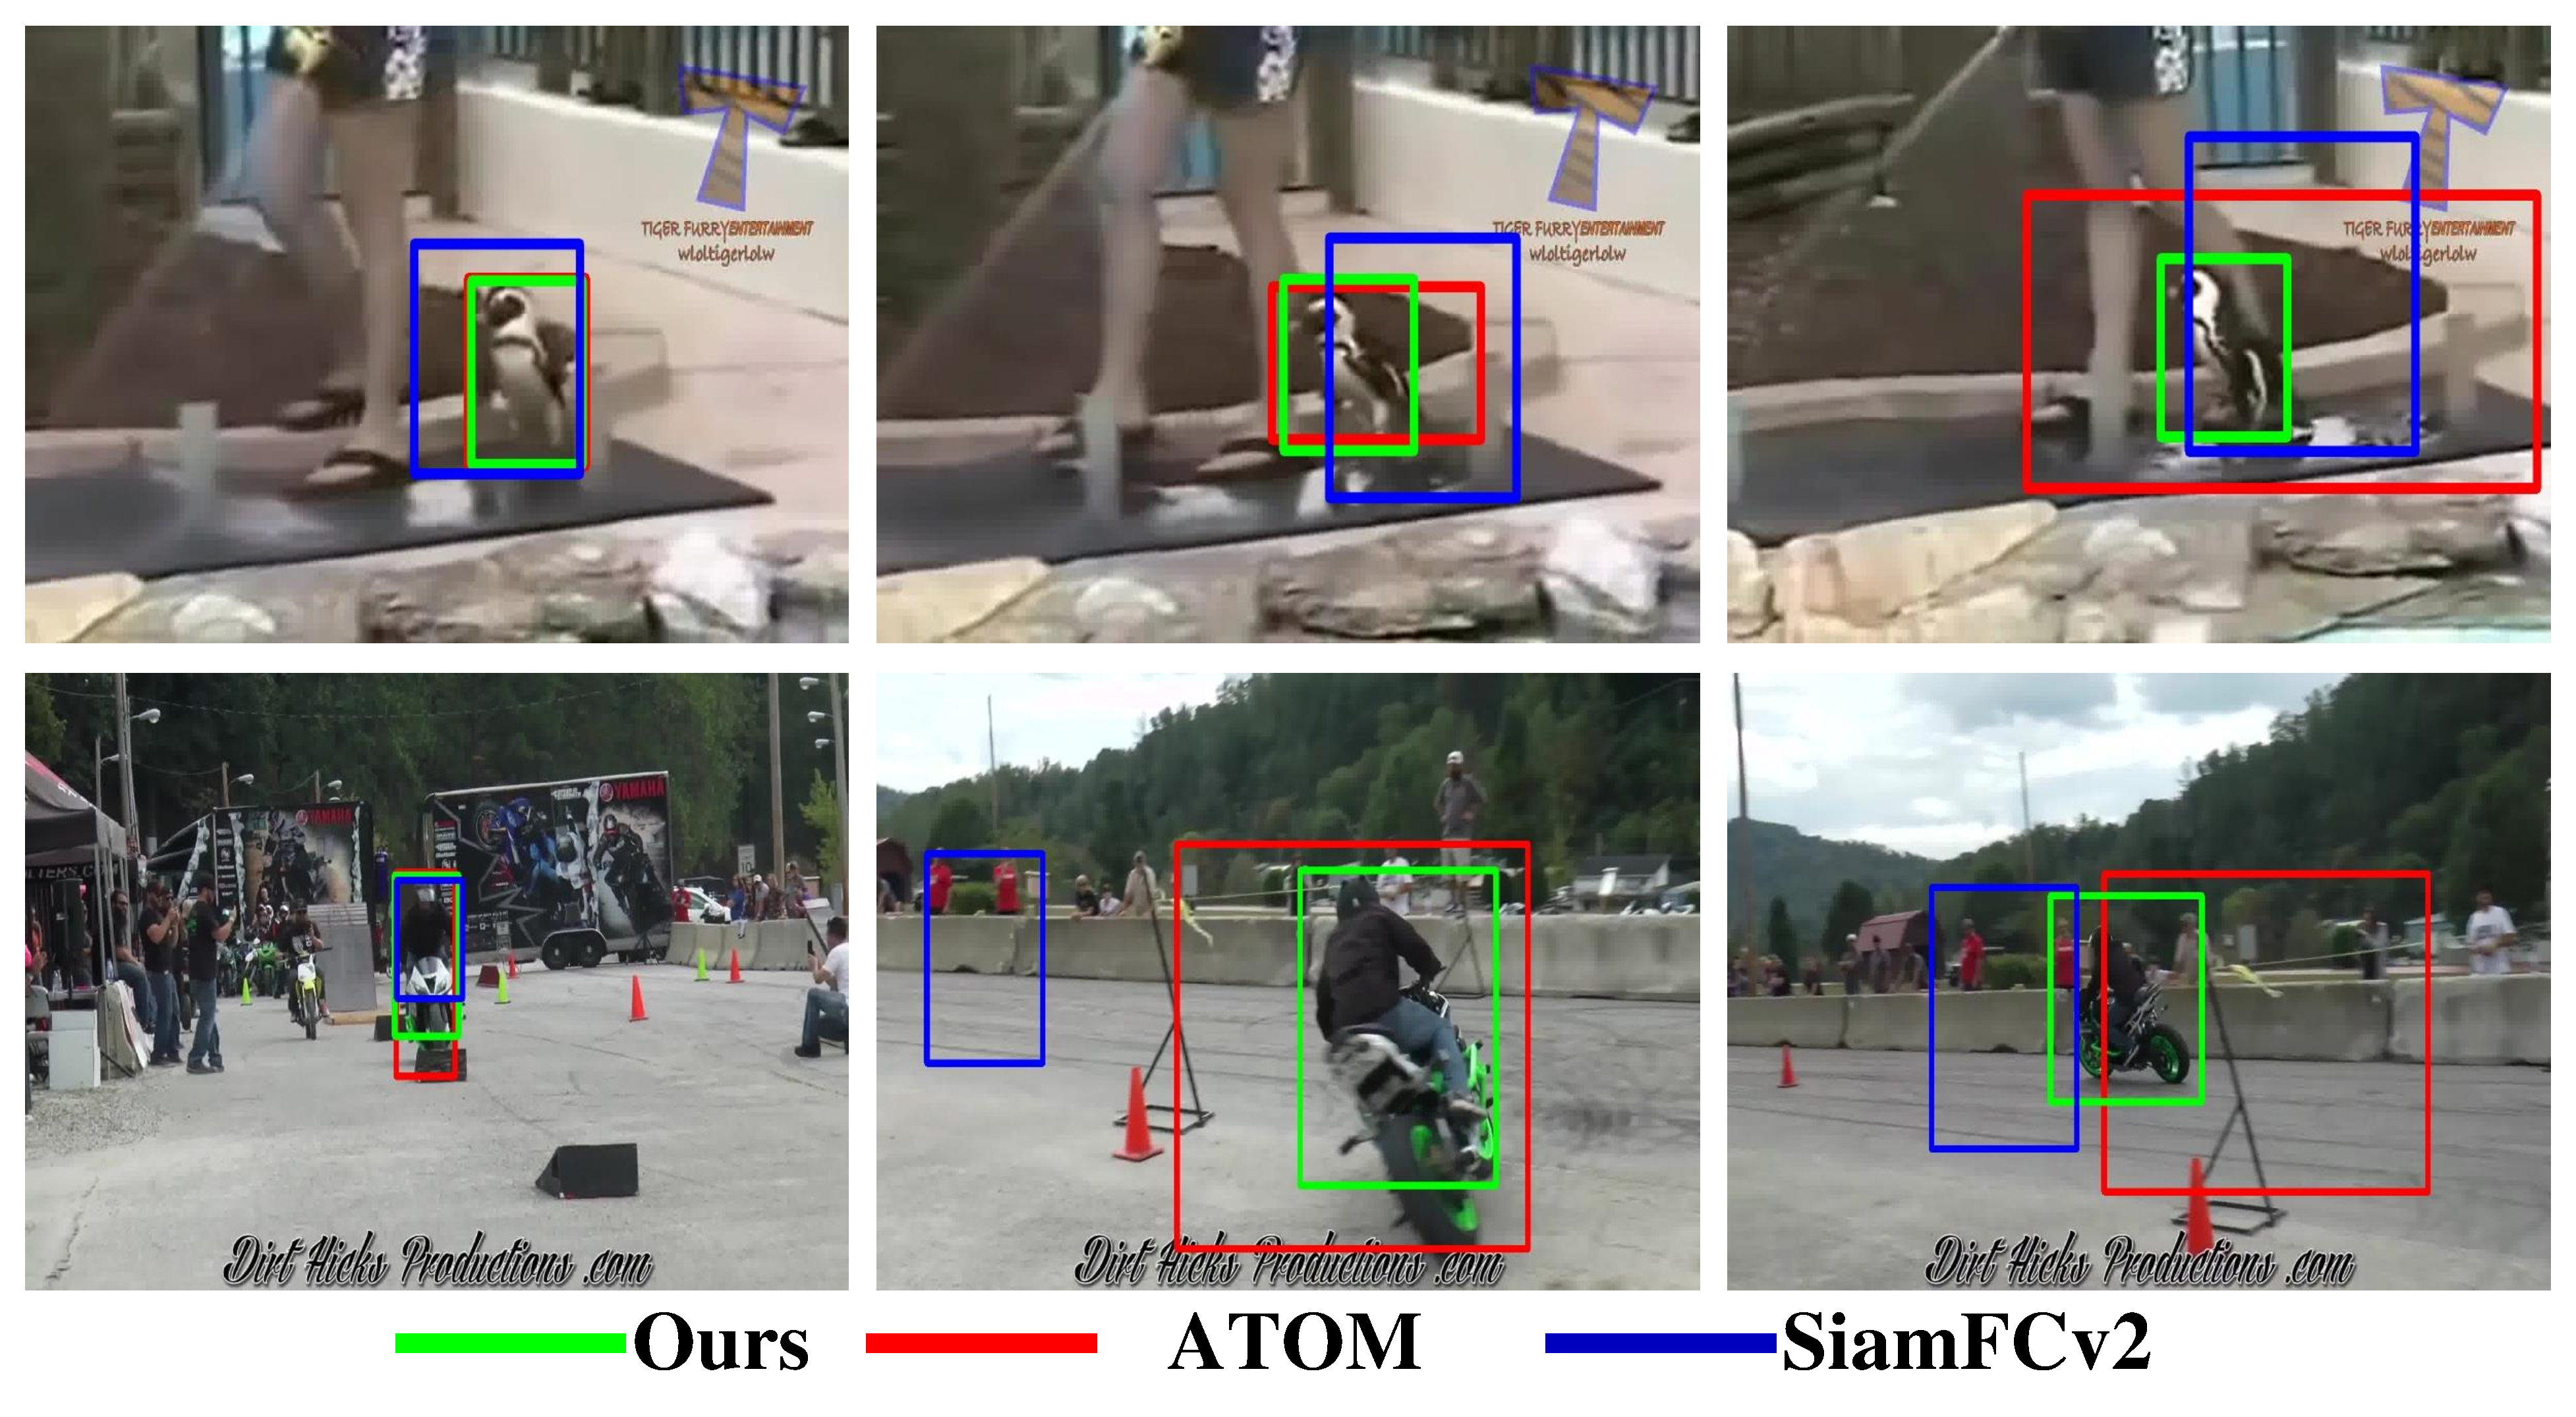
\includegraphics[width=1.0\textwidth]{Img/MTP/got10k/visulization2.pdf}
    \caption{本章提出的跟踪器与主流跟踪器 ATOM \cite{danelljan2019atom} 和 SiamFCv2 \cite{SiamFC} 在 GOT-10k \cite{GOT-10k} 测试集上的跟踪结果对比展示。}
    \label{fig:MTP_vis1}
\end{figure}
\fi

在本章中,我们表明视觉目标跟踪中具有挑战性的模型自适应任务可以通过简单地在孪生网络中操纵模板图像的像素来实现。给定一个视觉目标跟踪器,本章提出的算法使用第一帧中的目标真实标注框,仅在几次梯度下降迭代中修改模板像素。对于不包含在离线训练集中的目标,我们认为对模板图像像素进行微小修改可以改善离线训练的孪生网络的预测结果。我们使用对抗样本生成方法来实现此目的,因为对抗样本生成方法通常用于略微修改输入图像,从而对网络的预测结果产生影响。我们与对抗性样本生成的目的不同,因为后者旨在使网络预测变得更差,而我们希望孪生网络的预测更好。本章提出的模型自适应方法可以与各种孪生跟踪器(如 SiamFC++ \cite{SiamFC++})集成。在利用自适应信息提高跟踪性能的同时,孪生网络的参数保持不变,以保留离线训练的嵌入空间的表示能力。我们在 4 个视觉目标跟踪基准数据集上进行了全面的实验:VOT2018 \cite{kristan2018sixth}、TrackingNet \cite{muller2018trackingnet}、GOT-10k \cite{GOT-10k} 和 OTB2015 \cite{OTB2015}。本章提出的目标跟踪算法取得了较好的跟踪性能,同时以超过 80 FPS 的速度运行(见图 \ref{fig:MTP_vis})。
\section{相关工作}
模型更新是传统目标跟踪算法中的重要一环。然而,主流的孪生跟踪器通常采用离线训练的网络而不进行模型更新。由于没有在线学习,这些方法往往难以应对目标的表观变化和近似物体的干扰。
% UpdateNet
孪生网络跟踪器的基本原理是将目标表观模板的特征表示与测试帧中搜索区域的特征表示进行匹配。目标模板和搜索区域的特征是通过在大型数据集上离线训练的深度神经网络获取的。这种训练策略可以为跟踪任务提供出色的视觉描述符。在原始的孪生网络跟踪器 \cite{SiamFC} 中,目标模板在第一帧中初始化,然后在后续帧中保持固定。然而,目标表观的更改通常很大,不更新模板可能导致跟踪器过早失效。因此,使模型适应当前目标表观很重要。近年来,有一些算法尝试在孪生网络中进行模型更新。在文献 \cite{zhu2018distractor} 中,Zhu 等人提出使用简单的线性插值来更新每帧中的模板:
\begin{equation}
\widetilde{T}_{i}=(1-\gamma) \widetilde{T}_{i-1}+\gamma T_{i}.
\end{equation}
其中 $i$ 是帧的索引,$T_{i}$ 是仅使用当前帧计算的新模板样本,$\widetilde{T}_{i}$ 是累积的模板。通常,假设目标的表观在连续的帧中平滑且一致地变化,更新率 $\gamma$ 通常设置为较小的固定值(例如 $\gamma = 0.01$)。在孪生网络跟踪器中,$T$ 是由全卷积特征提取器从特定帧提取的目标表观模板。尽管模板平均提供了一种整合新表观的简单方法,但它也具有几个严重的缺点:

\begin{itemize}
\item 该方案对每个视频都采用恒定的更新速率,然而受多种因素(例如摄像机运动)的影响,不同视频的更新必要性不同。即使在同一视频中,目标模板所需的更新率也可能在不同时间中动态变化。
\item 更新率在模板的所有空间位置和所有通道上也是恒定的。然而在部分遮挡情况下,需要更新的仅仅是模板的一部分。
\item 跟踪器无法从漂移中恢复。部分原因是由于该方案无法访问初始表观模板 $T_{0}$,而初始表观模板 $T_{0}$ 是最可靠的模板。
\item 模板更新仅限于先前表观模板的简单线性组合。该策略限制了更新机制的灵活性,而这在目标经历复杂表观变化时非常重要。更复杂的模板特征组合方式可能有利于改善跟踪结果。
\end{itemize}

为了解决这些问题,在文献 \cite{Zhang_2019_ICCV} 中,Zhang 等人提出通过学习来对目标模板进行更新。学习的更新策略利用目标和图像信息。在该算法中,更新后的模板是根据以下内容计算的:(1)真实目标的初始模板,(2)所有先前帧的累积模板,以及(3)当前帧中预测的目标特征模板。因此,新的累积模板包含目标当前表观的有效历史信息,因为它会使用最新信息不断更新,同时由于使用了初始目标表观而增强了鲁棒性。上述模板更新算法使用卷积神经网络 UpdateNet 来实现。这是一个轻量卷积神经网络,可以与任何孪生跟踪器结合使用,以增强其在线更新能力,同时保持跟踪器的跟踪效率。
%此外,学习有效的模板更新的细微差别非常复杂,并且足够自适应以处理大量的跟踪情况。
在文献 \cite{DiscriminativeAnd} 中,Zhou 等人提出了一个基于注意力机制的在线更新模块,可以充分利用背景信息为孪生目标跟踪网络提取特定于目标的特征。具体而言,作者提出通过分数融合使用特定于目标的特征进行判别性学习,以帮助孪生网络处理近似物体和背景噪声的干扰。此外,作者提出通过模板更新使用特定于目标的特征提高其鲁棒性,以应对目标形变、旋转和光照变化等情况。该在线更新模块可以与各种孪生跟踪器集成在一起,而无需进行重新训练。%Discriminative and Robust Online Learning for Siamese Visual Tracking
在文献 \cite{FCOT} 中,Cui 等人为分类和回归分支设计提出了统一的全卷积架构(FCOT)。这种简单的跟踪方法不仅可以进行有效的训练和部署,还可以在两个分支上进行在线学习,以进行准确而强大的跟踪。具体而言,作者设计了一个回归模型生成器来在线优化回归模型,使回归分支能够有效处理目标形变,从而获得更精确的跟踪结果。此外,作者为分类分支设计了多尺度预测策略,以处理近似目标混淆的问题。通过从粗到精的融合,可以提高跟踪方法的精确性和鲁棒性。 %https://arxiv.org/pdf/2004.07109.pdf
在文献 \cite{TGGAN} 中,为了避免漂移问题并执行在线自适应,Guo 等人使用条件 GAN 架构 \cite{cGAN} 来学习目标的通用表观分布。在跟踪阶段,使用学习到的 GAN 生成器生成目标模板。生成器将第一帧中的真实目标模板和随机矢量作为输入,并输出生成的目标模板。生成的模板被真实目标模板约束,因此不会漂移。同时,生成的模板可以模拟目标可能产生的表观变化。跟踪时,选择最适合当前目标表观的生成模板。通过这些策略,可以在线更新目标模板,同时避免漂移。%Generating Reliable Online Adaptive Templates for Visual Tracking

\section{自适应信息增强的视觉目标跟踪算法}
在本节中,我们通过直接操纵模板像素为孪生跟踪器提供一种新的模型自适应方法。我们首先回顾基于模板匹配的主流跟踪器的跟踪过程。遵循文献 \cite{Danelljan_2020_CVPR},我们将目标跟踪形式化为基于置信度的回归问题,给定一个输出-输入对 $(\textbf y,\textbf x)$,该问题学习函数 $s_\theta:\mathcal{Y\times X\rightarrow \mathbb R}$,并预测标量置信度得分 $s_\theta(\textbf y,\textbf x)\in\mathbb R$。算法的最终预测 $f(\textbf x)=\textbf y^*$ 如下:
\begin{equation}
    f(\textbf x) = \arg\max_{\textbf y\in \mathcal Y}s_\theta (\textbf y,\textbf x),
\end{equation}
其中 $\textbf x$ 是输入图像。$\textbf y$ 通常表示目标的 2D 位置坐标。当前,有两种主流的基于模板匹配的跟踪框架:判别相关滤波器(discriminative correlation filter,DCF)方法和孪生跟踪方法。

基于 DCF 的方法在跟踪过程中训练循环相关滤波器 $w_{\theta}$ 来预测目标置信度得分:
\begin{equation}
    s_\theta(\textbf y,\textbf x)=(w_\theta \star \phi(\textbf x))(\textbf y),
    \label{equ:dcf}
\end{equation}
其中 $\phi(\textbf x)$ 是从搜索图像 $\textbf x$ 中提取的特征,$\star$ 表示相关操作。

与 DCF 相比,孪生跟踪器采用双流体系结构。一个流根据模板图像 $\textbf z$ 提取目标的特征 $\phi_\theta(\textbf z)$,该模板图像是根据真实边界框从第一帧裁剪而来的。另一个流接收较大的搜索图像 $\textbf x$ 作为输入,并输出搜索特征 $\phi_\theta(\textbf x)$。这两个输出进行互相关以预测目标置信度得分:
\begin{equation}
    s_\theta(\textbf y,\textbf x)=(\phi_\theta(\textbf z) \star \phi_\theta(\textbf x))(\textbf y).
    \label{equ:siamese}
\end{equation}

基于 DCF 的跟踪器和孪生跟踪器都具有利用大规模视觉目标跟踪数据集来训练特征提取器 $\phi(\cdot)$ 或嵌入网络 $\phi_{\theta}(\cdot)$ 的优势。因此,可以增强特征在目标跟踪任务上的表示能力。

与孪生跟踪器不同,DCF 利用目标模板图像学习滤波器 $w_\theta$,以将其与背景区分开。
尽管使用了循环相关运算提高了跟踪效率,但由于边界效应和复杂的优化使 DCF 无法在计算速度和跟踪性能之间做出良好的平衡。孪生跟踪器在这方面做得更好,然而在互相关中学习到的相似性度量对于未包含在离线训练集中的目标不一定是可靠的,从而导致泛化性较差。

在本章中,我们旨在设计一种新的孪生跟踪方法,该方法可以像基于 DCF 的跟踪器一样充分利用当前视频的特定信息进行模型自适应,尽管其中的目标可能并不包含在离线训练时使用的训练集中。我们通过利用第一帧中的注释信息执行模型自适应调整来实现这一目的。

注意公式 \ref{equ:dcf} 和公式 \ref{equ:siamese} 之间存在相似之处,主要区别在于进行相关计算的核:DCF 的核是在线学习的 $w_{\theta}$ ,而孪生网络的核是 $\phi_\theta(\textbf z)$。为了使孪生网络具有模型自适应能力,我们需要使用当前视频的第一帧标注信息来自适应调整 $\phi_\theta(\textbf z)$。调整 $\phi_\theta(\textbf z)$ 有两种设计选择:更改 $\phi_\theta(\cdot)$ 或更改 $\textbf z$。但是,更改 $\phi_\theta(\cdot)$ 可能会导致繁琐的元学习设置,难以确保离线训练的嵌入空间 \cite{ROAM, MetaRTT} 的特征表示能力。相反,我们的解决方案是以简单的方式通过更改 $\textbf z$ 来执行孪生跟踪器的模型自适应,即在第一帧使用目标真实标注信息仅在几次梯度下降迭代中修改模板像素。与当前的孪生跟踪模型自适应方法相比,该方法具有以下优点:

\begin{itemize}
\item 首先,我们不修改孪生网络的参数,从而保留离线训练的嵌入空间的表示能力。
\item 其次,与旨在合并先前帧目标特征的模板更新方法 \cite{zhu2018distractor, Zhang_2019_ICCV} 不同,我们专注于在第一帧使用目标真实标注信息进行初始自适应。
\item 最后,在不改变基线跟踪器整体架构的情况下,我们的模型自适应方法即插即用,易于实现。
\end{itemize}

在下一节中,我们将展示如何使用对抗样本生成方法来执行用于模型自适应的模板像素操纵。

\subsection{操纵模板像素以进行模型自适应}
乍看之下,模型自适应任务与对抗样本生成任务之间可能存在矛盾,因为这两个任务具有不同的目的。对抗样本 \cite{kurakin2017adversarial} 是对输入数据进行微小修改后的样本,目的是对机器学习系统进行攻击,导致机器学习模型做出错误的预测。然而,模型自适应的目的是在第一帧中充分利用注释信息,以提高当前视频的跟踪性能。接下来,我们将指出这两个任务之间存在一些相似之处,并且我们可以利用对抗样本生成方法来执行模型自适应任务。

在介绍提出的方法之前,我们首先回顾流行的对抗样本生成方法。生成对抗图像 $I^{adv}$ 的最简单方法之一是通过线性化干净图像的 $L_{\infty}$ 邻域中的损失函数,并使用以下闭式方程进行求解 \cite{FGSM}:
\begin{equation}
    I^{adv} = I + \epsilon \text{ sign} \bigl( \nabla_I L(I, y_{true})  \bigr),
\end{equation}
其中 $I$ 是输入图像,像素值是 [0,255] 范围内的整数。 $y_{true}$ 是图像 $I$ 的真实标签。给定图像 $I$ 和标签 $y$,$L(I, y)$ 是用于攻击神经网络的损失函数。$\epsilon$ 是超参数。扩展上述方法的一种直接方案是,以较小的步长迭代应用该公式,并在每次迭代之后裁剪中间结果的像素值,以确保位于原始图像的 $\epsilon$ 邻域中。该方法即在文献 \cite{kurakin2017adversarial} 中提出的基本迭代方法(BIM):
\begin{equation}
    \begin{gathered}
        I_0^{adv} = I, \\
        I_{N+1}^{adv} = Clip_{I,\epsilon}\{I_N^{adv}+\alpha \text{ sign}(\nabla_I L(I_N^{adv},y_{true}))\},
    \end{gathered}
\end{equation}
其中 $Clip_{I, \epsilon} \left\{ I' \right\}$ 用于对图像 $I'$ 进行逐像素裁剪,从而保证结果在原始图像 $I$ 的 $\epsilon$ 邻域内。
BIM 可以进行扩展以攻击特定的期望目标类别 \cite{kurakin2017adversarial}:
\begin{equation}
    \begin{gathered}
        I_0^{adv} = I,\\
        I_{N+1}^{adv} = Clip_{I,\epsilon}\{I_N^{adv}-\alpha \text{ sign}(\nabla_I L(I_N^{adv},y_{target}))\}.
    \end{gathered}
    \label{equ:itcm}
\end{equation}
公式 \ref{equ:itcm} 表明,仅需进行几次梯度下降迭代操作对输入图像的像素进行修改,就可以将网络的预测更改为特定类别 $y_{target}$。请注意,我们的目的是在第一帧中修改模板图像的像素,以使预测更接近于真实边界框。因此,我们可以对公式 \ref{equ:itcm} 进行一些修改,用于对孪生网络进行模型自适应:
\begin{equation}
    \begin{gathered}
        \textbf z_0 = \textbf z,\\
        \textbf z_{N+1} = Clip_{\textbf z,\epsilon}\{\textbf z_N -\alpha \text{ sign}(\nabla_{\textbf z} L(\textbf z_N,y_{bb}))\},
    \end{gathered}
    \label{equ:adaptaion}
\end{equation}
其中 $\textbf z$ 是第一帧中的模板图像,而 $y_{bb}$ 是根据真相边界框生成的孪生跟踪器的标签。在下一节中,我们将介绍配备了所提出的模型自适应模块的跟踪器的整体跟踪过程。

%%%%%%%%%%%%%%%%
\begin{table}[t]
\caption{本章提出的跟踪算法与相关算法在视觉目标跟踪数据库 OTB2015 上的评测结果。跟踪器速度在 NVIDIA RTX 2080Ti GPU 上进行测试。}
\setlength{\tabcolsep}{3pt}
\begin{center}
\begin{tabular}{c c c c c c c}
\toprule
跟踪器 & 
\begin{tabular}{c} ECO  \\ \cite{danelljan2017eco} \end{tabular} &
\begin{tabular}{c} MDNet \\ \cite{MDNet} \end{tabular} &
\begin{tabular}{c} SiamRPN++ \\ \cite{SiamRPN++} \end{tabular} &
\begin{tabular}{c} ATOM \\ \cite{danelljan2019atom} \end{tabular} &
\begin{tabular}{c} SiamFC++ \\ \cite{SiamFC++} \end{tabular} &
本章算法 \\
%跟踪器 & ECO \cite{danelljan2017eco} & MDNet \cite{MDNet} & SiamRPN++ \cite{SiamRPN++} & ATOM \cite{danelljan2019atom} & SiamFC++\_G \cite{SiamFC++} & 本章算法 \\
\midrule
成功率 & 70.0 & 67.8  & 69.6      & 66.9      & 68.3       & 69.7 \\
速度(FPS)     & 8    & 1     & 35        & 30       & 90         & 82  \\
\bottomrule
\end{tabular}
\end{center}
\label{table:otb}
\end{table}
%%%%%%%%%%%

%%%%%%%%%%%%%%%%%%%%%%%%%%%%%%%
\subsection{跟踪框架}
所提出的模型自适应方法以即插即用的方式与 SiamFC++ 跟踪器 \cite{SiamFC++} 集成在一起。 SiamFC++ 基于 SiamFC \cite{SiamFC},并根据文献 \cite{SiamFC++} 中提出的一些准则逐步完善。原始 SiamFC++ 网络的输入由从第一帧裁剪的模板图像 $\textbf z_0$ 和从第 $i$ 帧裁剪的搜索图像 $\textbf x_i$ 组成。但是,我们希望执行模板像素操纵,以便在对输入对 $(\textbf z_0, \textbf x_0)$ 进行 $N$ 步像素更新获得 $\textbf z'$ 后,跟踪器在 $(\textbf z', \textbf x_i)$ 上表现良好。为此,我们首先在第一帧根据目标的真实标注框裁剪初始模板图像 $\textbf z_0\in\mathbb R^{3\times128\times 128}$ 和初始搜索图像 $\textbf x_0\in\mathbb R^{3\times303\times 303}$。
然后,将 $\textbf z_0$ 和 $\textbf x_0$ 发送到 SiamFC++ 网络以获得第一帧的跟踪预测。SiamFC++ \cite{SiamFC++} 中的跟踪损失计算如下:
\begin{equation}
    L = L_{\text{cls}} + L_{\text{quality}} + L_{\text{reg}},
\end{equation}
其中 $L_{\text{cls}}$ 是焦点损失 \cite{focal}。$L_{\text{quality}}$ 是用于质量评估的二进制交叉熵(BCE)损失。$L_{\text{reg}}$ 是边框回归的 IoU 损失 \cite{yu2016unitbox}。根据公式 \ref{equ:adaptaion},相对于模板 $\textbf z_0$ 的梯度用于生成 $\textbf z_1$。通过应用少数几次迭代可以获得更新的模板 $\textbf z'$(公式 \ref{equ:adaptaion})。请注意,模板图像仅使用给定序列的第一帧进行更新,并在整个跟踪过程中保持固定以确保稳定性。
后续跟踪过程与 SiamFC++ 相同。

\section{实验评估与分析}
\begin{table}[t]
\caption{本章提出的算法在数据集 OTB2015 \cite{OTB2015}、VOT2018 \cite{kristan2018sixth}、GOT-10k \cite{GOT-10k}、TrackingNet \cite{muller2018trackingnet} 上的评测结果。}
\begin{center}
\begin{tabular}{c cc c}
\toprule
跟踪器 & 评价指标 & 基线方法 & 本章方法\\
\midrule
\multirow{1}{*}{OTB2015 \cite{OTB2015}} 
& Success & 68.3 & 69.7\\
\midrule
\multirow{3}{*}{VOT2018 \cite{kristan2018sixth}}
& A   & 0.587 & 0.591 \\
& R   & 0.183 & 0.187 \\
& EAO & 0.426 & 0.438 \\
\midrule
\multirow{3}{*}{GOT-10k \cite{GOT-10k}} 
& SR\textsubscript{0.50} &  0.737 & 0.748 \\
& SR\textsubscript{0.75} & 0.464 & 0.475 \\
& AO & 0.607 & 0.617 \\
\midrule
\multirow{3}{*}{TrackingNet \cite{muller2018trackingnet}} 
& Prec.       & 70.5 & 70.6 \\
& Norm. Prec. & 80.0 & 81.7 \\
& Succ.       & 75.4 & 74.9 \\
\midrule
\multicolumn{2}{c}{FPS} & 90 & 82\\
\bottomrule
\end{tabular}
\end{center}
\label{tab:benchmark results}
\end{table}
%%%%%%%%%%%

%%%%%%%%%%%%%%%%%
\begin{figure}[t]
    \centering
    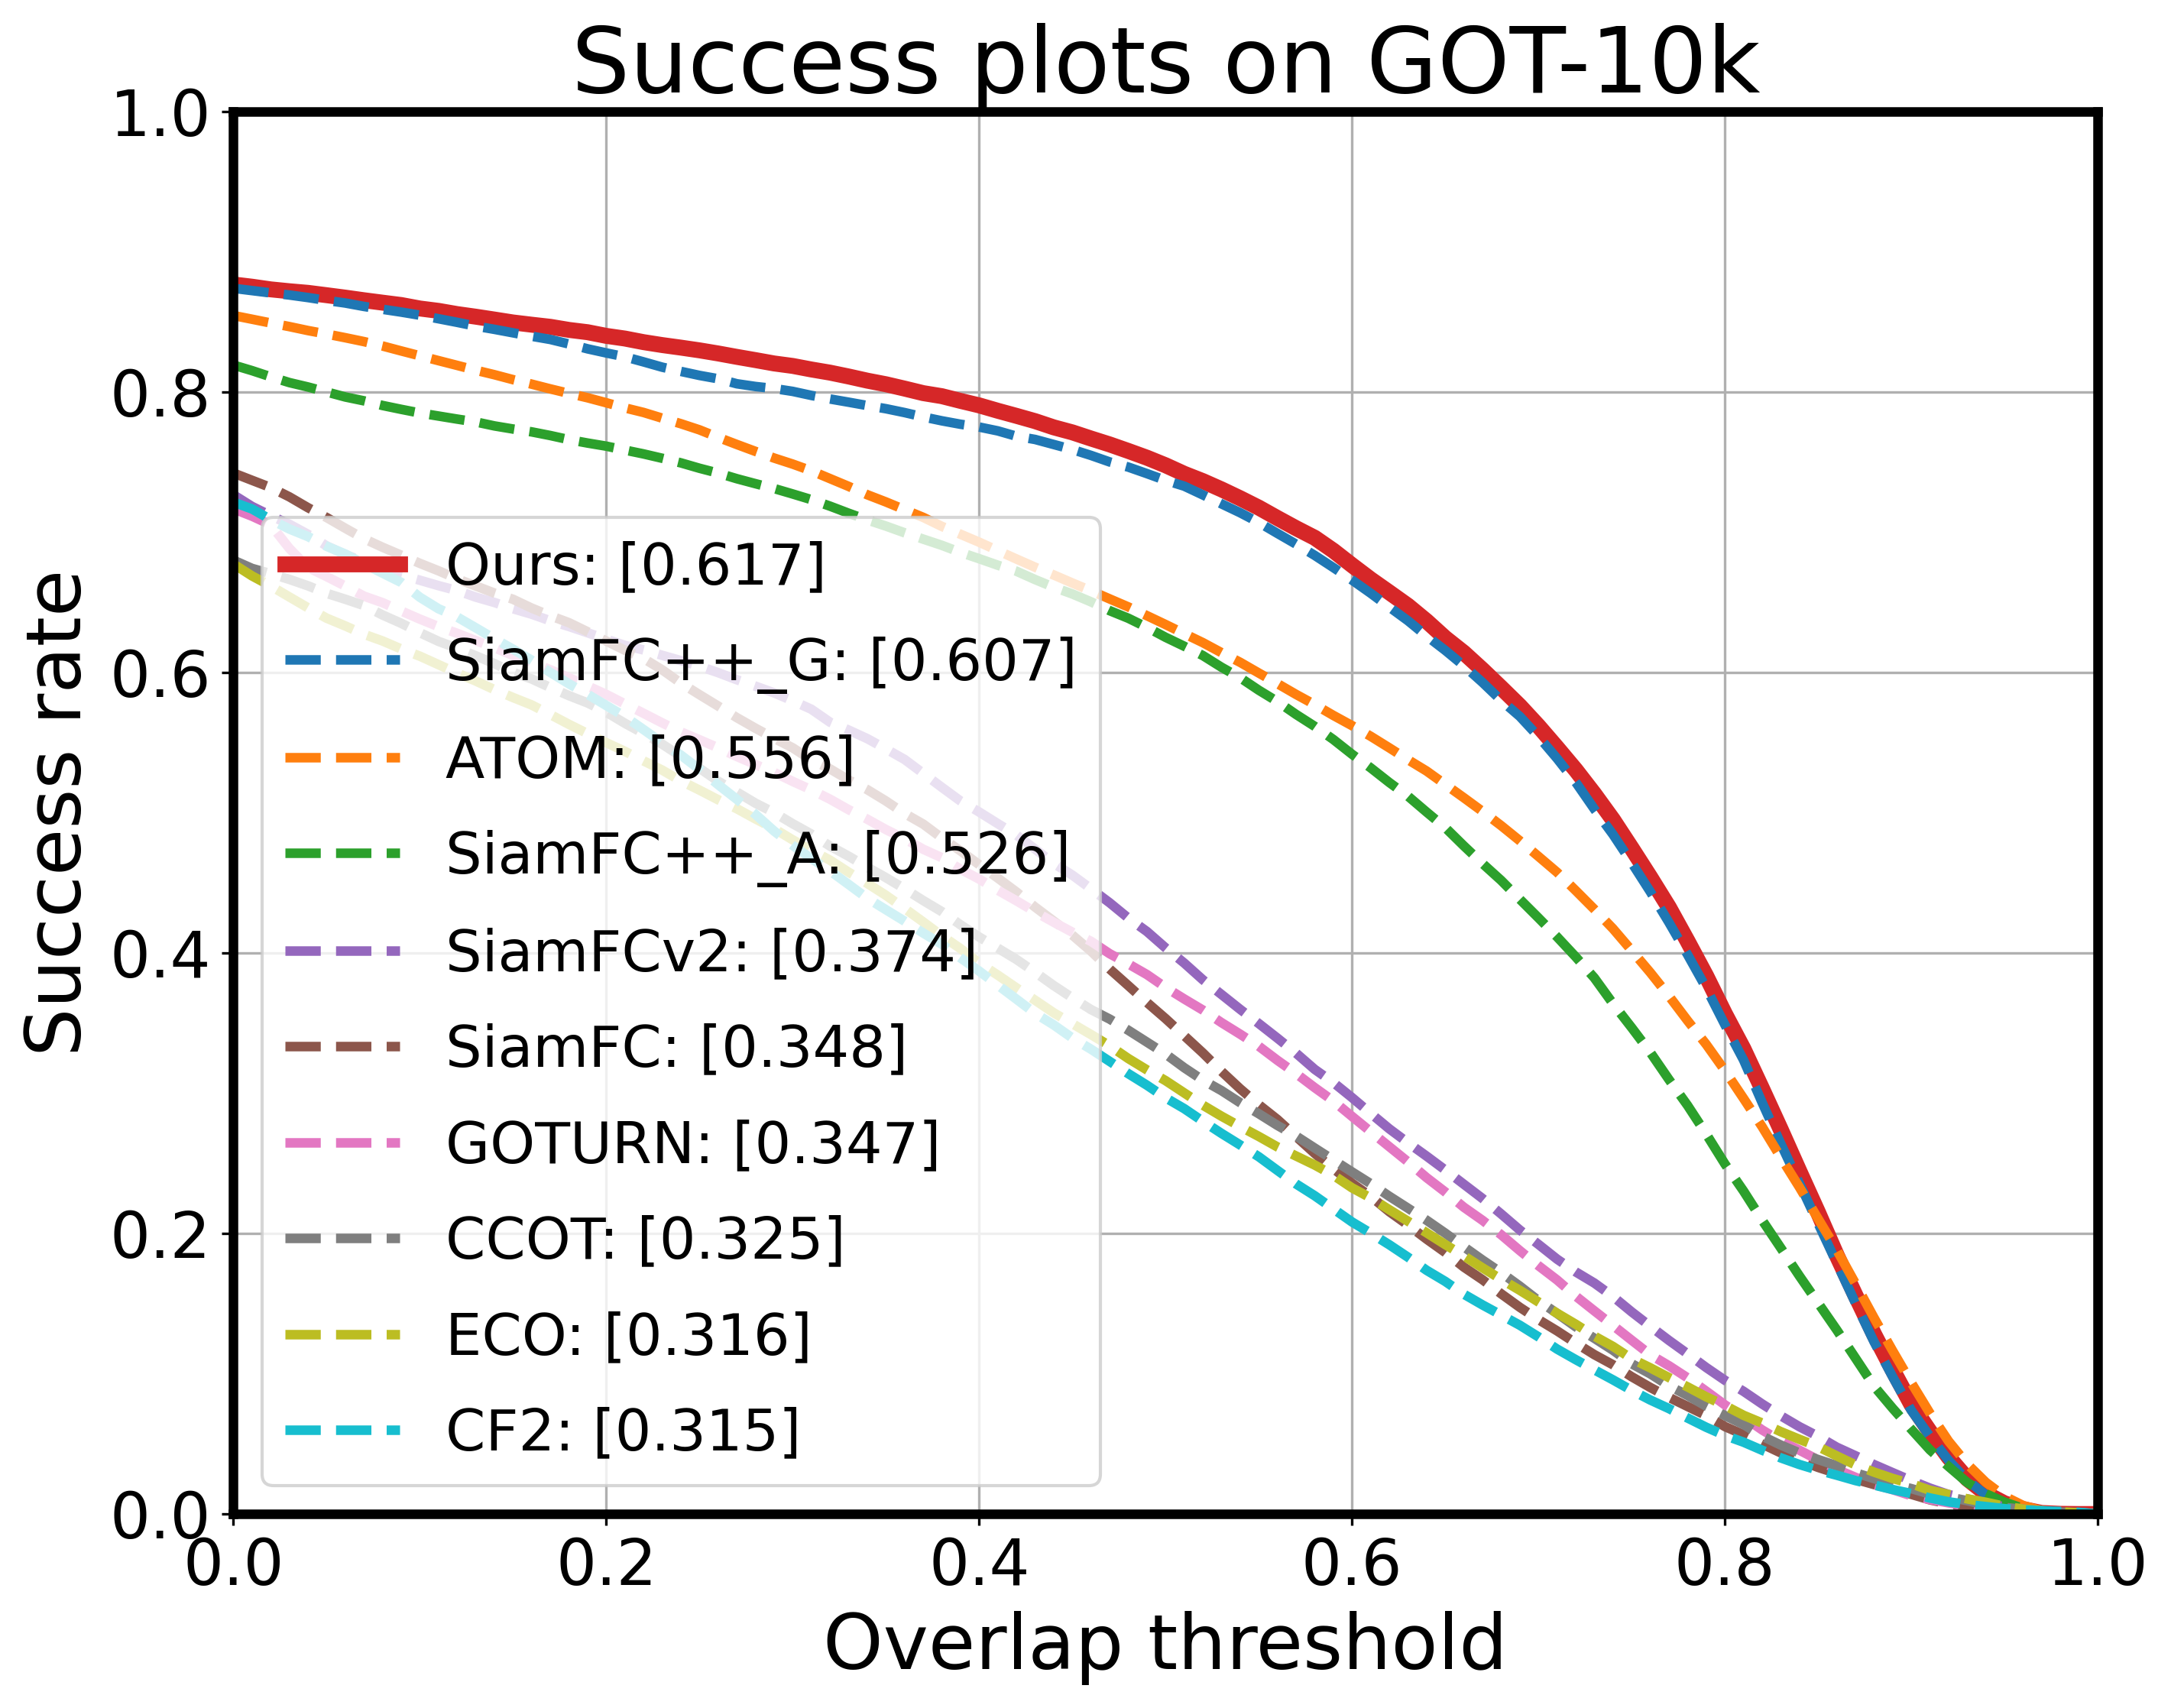
\includegraphics[width=0.75\textwidth]{Img/MTP/got10k/success_plot.png}
    \caption{GOT-10k \cite{GOT-10k} 测试集中算法的平均重叠率(AO)排序图。}
    \label{fig:got10k}
\end{figure}
%%%%%%%%%%%%

\begin{figure}[p]
    \centering
    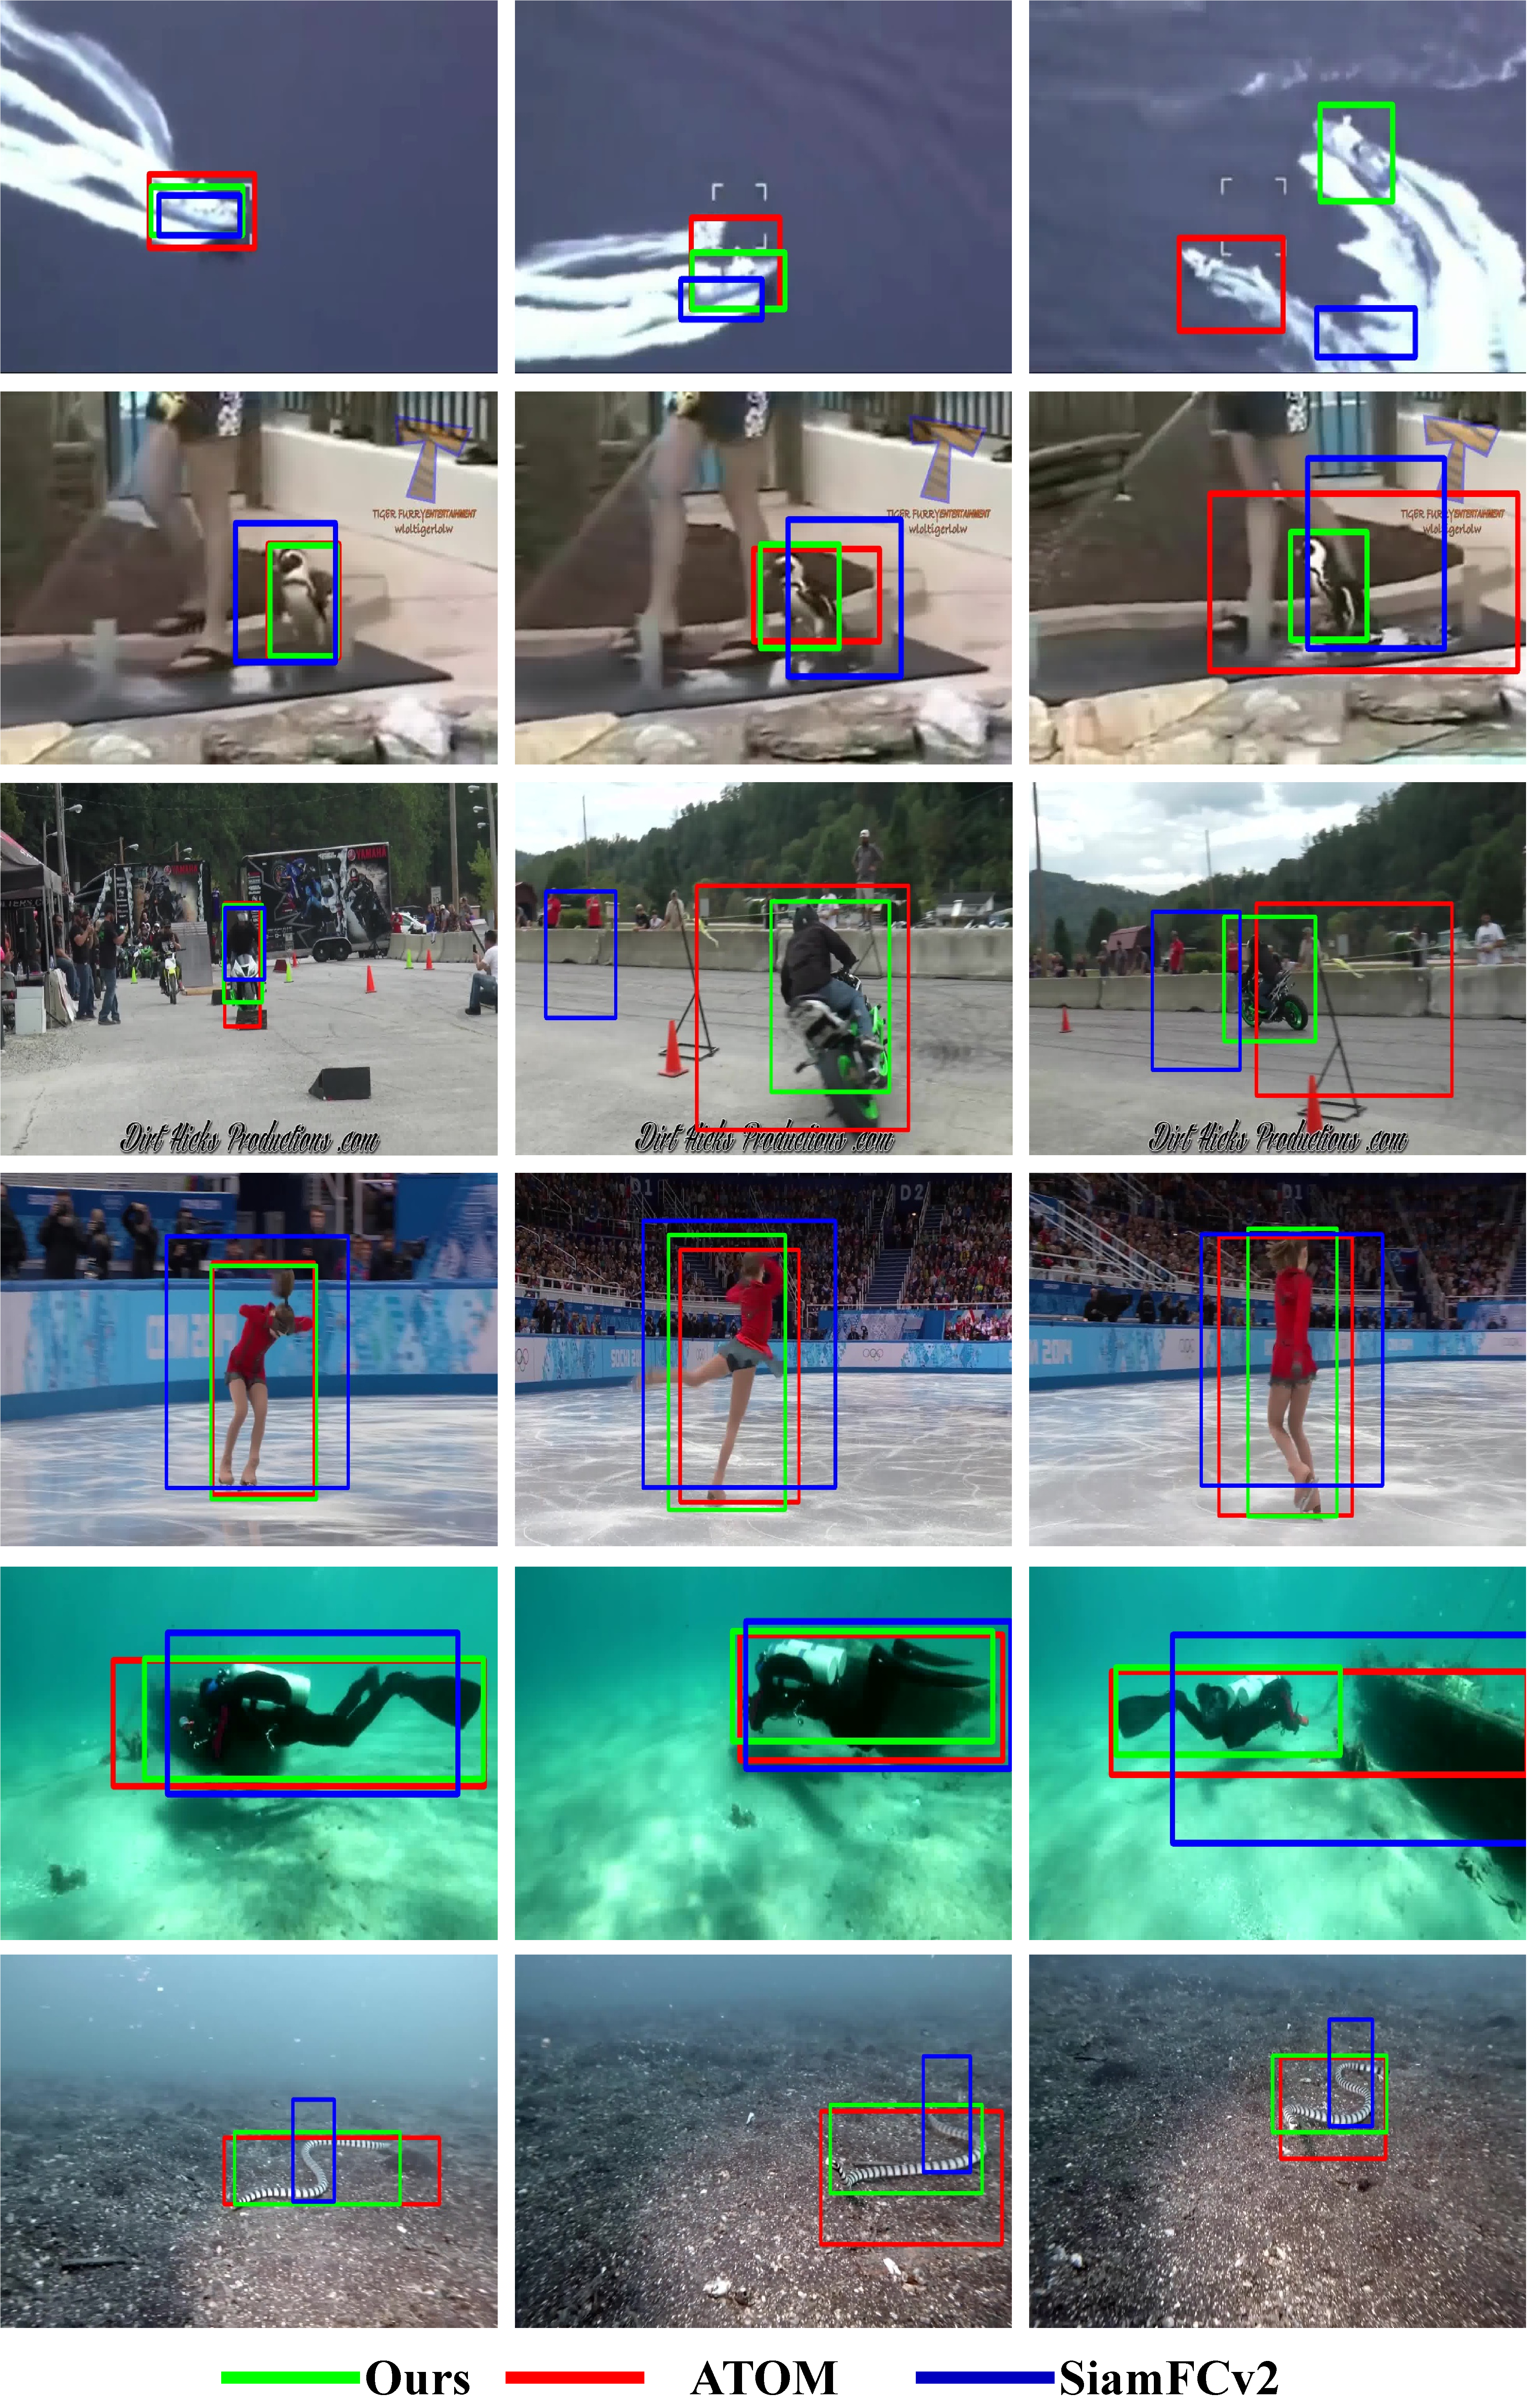
\includegraphics[width=0.99\textwidth]{Img/MTP/got10k/visulization.pdf}
    \caption{本章提出的跟踪器与主流跟踪器 ATOM \cite{danelljan2019atom} 和 SiamFCv2 \cite{SiamFC} 在 GOT-10k \cite{GOT-10k} 测试集上的跟踪结果对比展示。}
    \label{fig:MTP_vis}
\end{figure}

\begin{figure}[t!]
    \centering
    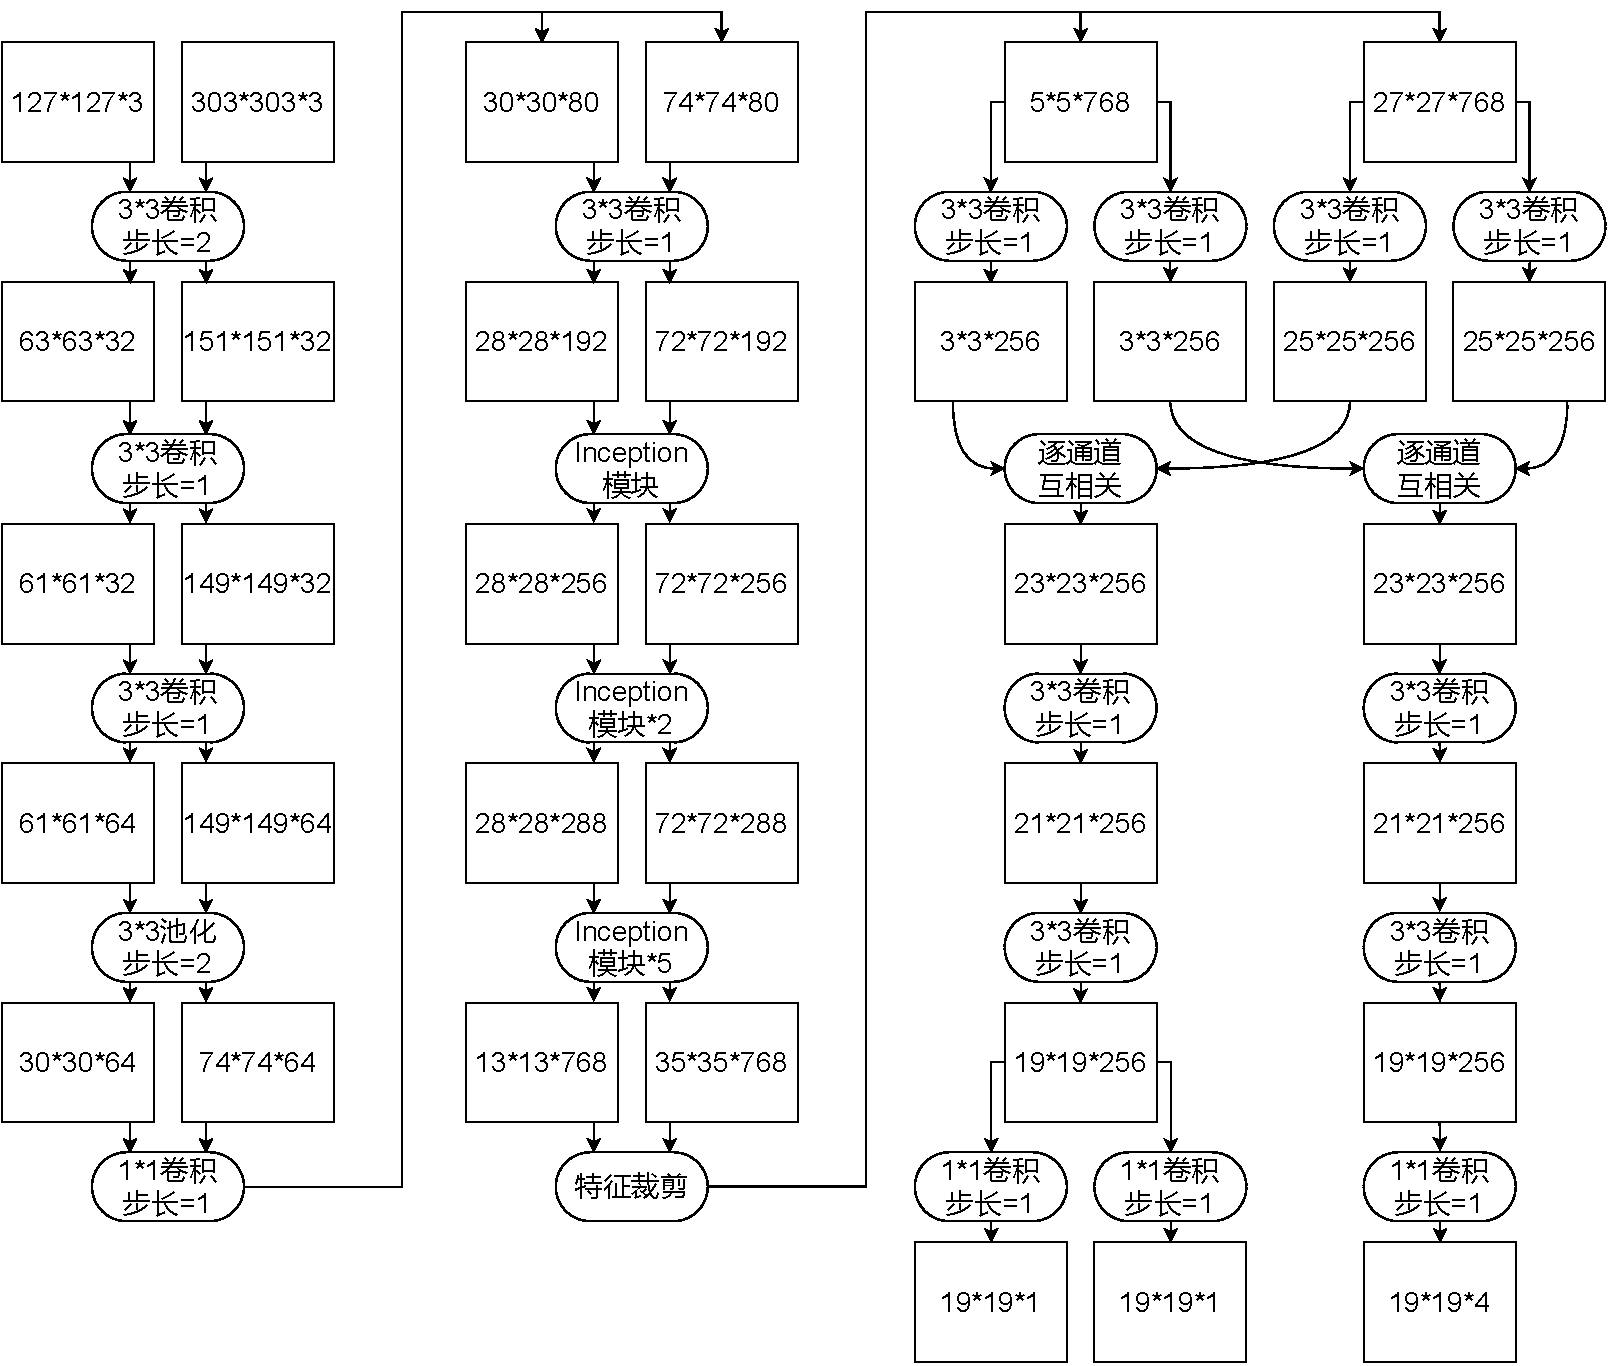
\includegraphics[width=0.99\textwidth]{Img/MTP/SiamFC++.pdf}
    \caption{本章采用的基线孪生网络结构参数示意图。}
    \label{fig:MTP_SiamFC++}
\end{figure}

\subsection{实验设置}
\textbf{网络架构设计}:本章所采用的基线孪生目标跟踪网络主要由四个子网络组成,分别是用于共享特征提取的主干网络,用于预测边框位置的回归子网络,用于判断目标出现可能性的分类分支,以及用于预测边框质量的质量评估分支。网络结构如图 \ref{fig:MTP_SiamFC++} 所示。主干网由 5 个卷积层和 8 个 Inception 块 \cite{GoogLeNet} 构成,可为模板图像和搜索图像提取高层语义信息,以提升跟踪精度。

\textbf{训练数据}:为了提高特征表示的泛化能力和判别能力,同时避免在稀缺的跟踪数据上过度拟合,基线网络的离线训练数据集包括 ILSVRC-VID/DET \cite{VID}、COCO \cite{COCO}、YoutubeBB \cite{YTBB}、LaSOT \cite{LaSOT} 和 GOT-10k \cite{GOT-10k}。
其中,大规模视觉识别挑战赛(imagenet large scale visual recognition challenge,ILSVRC)数据集包含超过 4000 个视频序列以及约 130 万个矩形框标注,具有较为丰富多样的视频场景分布。
COCO 数据集是一个大型的、丰富的物体检测、分割和图像描述数据集。该数据集以场景理解为目标,主要从复杂的日常场景中截取,图像中的目标通过精确的分割进行位置的标定。图像包括 91 类目标,328000 幅图像和 2500000 个标签。
YoutubeBB 数据集是带有高质量单目标边框注释的大规模数据集,从 240000 段 YouTube 视频中提取大约 380000 个时长 15 秒至 20 秒的视频片段。所选择的视频大多以手持设备(如手机摄像头)拍摄,未进行编辑和后处理。所有视频片段标注有高精度的分类标签,并以 1 帧每秒的帧率进行人工边框标注。该数据集的目的是推动机器学习的进展,以促进视频理解。
LaSOT 数据集是一个具有高质量手动密集标注的目标跟踪数据集,包含 1400 个视频,每个序列平均 2512 帧。每一帧都经过仔细检查和手动标记,并在需要时对结果进行目视检查和纠正,从而生成大约 352 万个高质量的边界框标注。LaSOT 共包含 70 个类别,每个类别包含 20 个序列。
GOT-10k \cite{GOT-10k} 包括超过一万个视频片段,分为 563 类运动目标和 87 类运动模式,以尽可能覆盖现实情况中的各种挑战性模式,并带有超过 150 万个手动标记的边界框,从而可以对深度跟踪器进行统一训练和稳定评估。在 GOT-10k 采用的跟踪器评估协议中,训练集和测试集的物体类别是零重叠的。该协议避免了评估结果的偏差。
上述数据集被广泛使用在最近提出的孪生网络跟踪算法 \cite{SiamRPN++,Wang2018SiamMask} 的训练中。
对于视频数据集 VID、LaSOT 和 GOT-10k,从间隔小于 100 帧内抽取图像对。对于视频数据集 YoutubeBB,从间隔小于 5 帧内抽取图像对。对于图像数据集 COCO 和 ILSVRC-Det,生成负样本对作为训练样本的一部分,以增强模型区分近似目标的能力。在搜索图像上按均匀分布指定随机平移和缩放以进行数据增强。

\textbf{优化器参数设定}:对于基线网络的训练,使用动量为 0.9 的随机梯度下降(stochastic gradient descent,SGD)优化器对网络参数进行训练,并将权值衰减参数设置为 0.0005。
模型经过 20 个迭代周期的训练,每个迭代周期中图像对的数量为 300000 对。
主干网络中的参数在前 10 个迭代周期中被冻结,并从第 11 个迭代周期开始进行训练以避免过拟合。
模型的全局学习率为 $2\times 10^{-2}$。主干网络中参数的学习率为全局学习率的十分之一。
公式 \ref{equ:adaptaion} 中的参数 $\alpha$ 设为 0.05。

\textbf{测试阶段}:测试时,除利用自适应信息对模板像素进行调整外,不对基线网络进行任何更改。测试阶段的模型输出是一组带有置信度得分的边界框。根据边界框的尺度/长宽比变化以及距上一帧中预测目标的位置,对置信度得分进行惩罚,最后选择得分最高的边界框用于更新目标状态。

本章所提出的自适应信息增强的孪生网络跟踪器使用 PyTorch 在 Python 中实现,所有实验在装配有 Intel(R) Xeon(R) CPU E5-2630 v4 @ 2.20GHz
和 NVIDIA RTX 2080Ti GPU 的工作站上执行。本章提出的跟踪器在 NVIDIA RTX 2080Ti GPU 上以超过 80 FPS 的速度运行。

%%%%%%%%%%%%%%%%%
\begin{figure}[t]
    \centering
    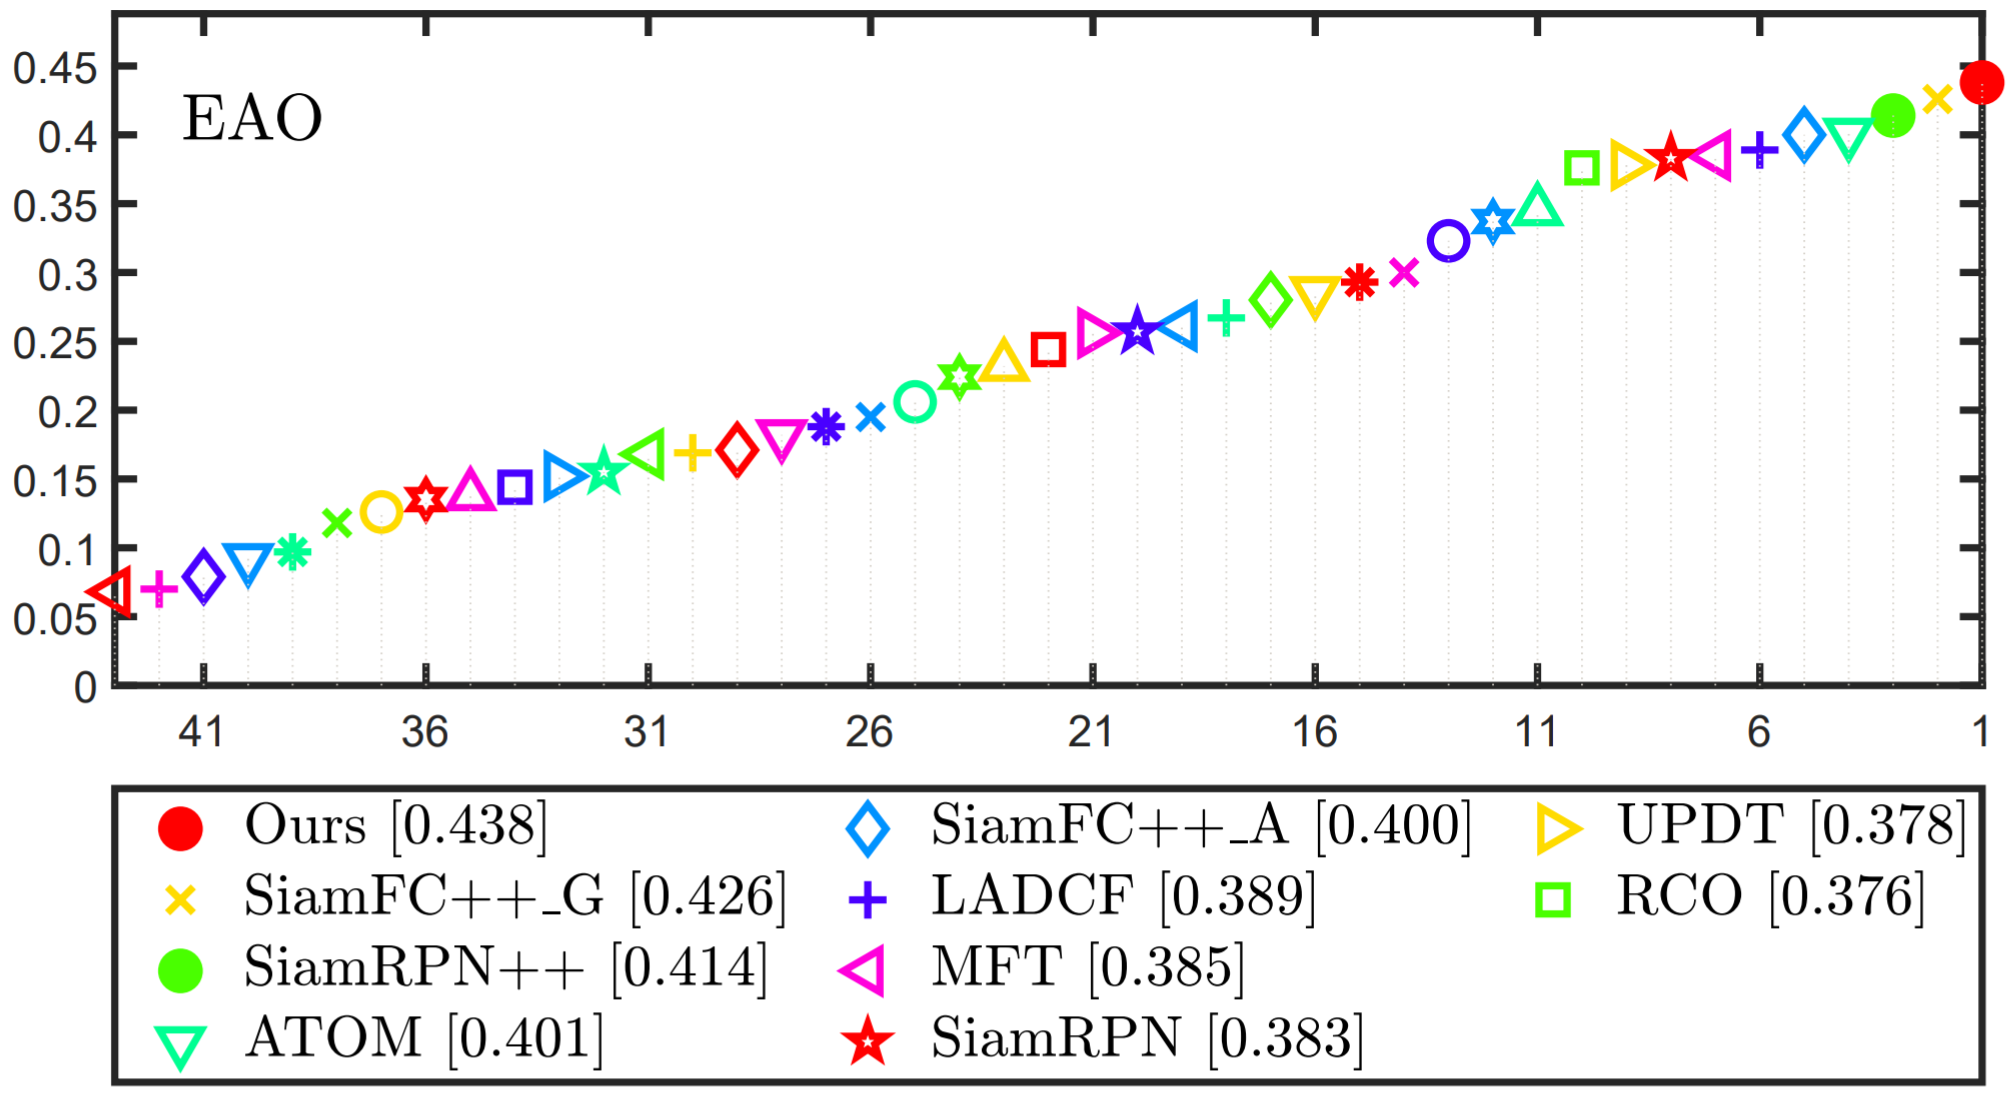
\includegraphics[width=1.0\textwidth]{Img/MTP/vot18/vot18_eao.png}
    \caption{数据集 VOT2018 中算法的期望平均重叠率(EAO)排序图。}
    \label{fig:eao}
\end{figure}
%%%%%%%%%%%%


%%%%%%%%%%%%%%%%%%%%%%%%%%%%%%%%%%%%%
\subsection{与主流跟踪器的比较}

在本节中,我们将本章提出的方法与主流跟踪器在四个跟踪数据集上进行比较:OTB2015 \cite{OTB2015},VOT2018 \cite{kristan2018sixth},GOT-10k \cite{GOT-10k} 和 TrackingNet \cite{muller2018trackingnet}。具体来说,OTB2015 \cite{OTB2015} 包含 100 个序列,这些序列标记有不同的属性,用于深入分析跟踪性能。VOT2018 \cite{kristan2018sixth} 独特地应用了基于重置的方法,并挑选了 60 个序列对各种跟踪方案进行评估。GOT-10k \cite{GOT-10k} 和 TrackingNet \cite{muller2018trackingnet} 是最近提出的两个视觉目标跟踪数据集。它们在训练和测试集中涵盖了各种目标类和场景。对于 GOT-10k,训练和测试集之间的目标类别没有重叠,从而可以有效评估跟踪器对目标类别的泛化能力。

\iffalse
\begin{figure*}[p]
\begin{center}
\subfloat[]{
	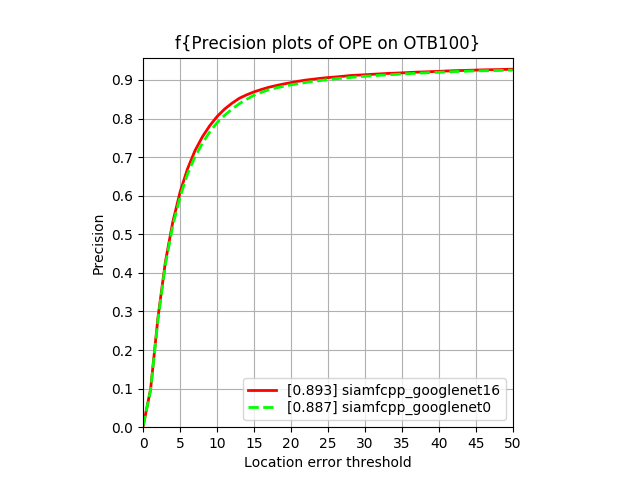
\includegraphics[width=0.33\textwidth]
	{Img/MTP/otb2015/precision_ALL.png}
}
\subfloat[]{
	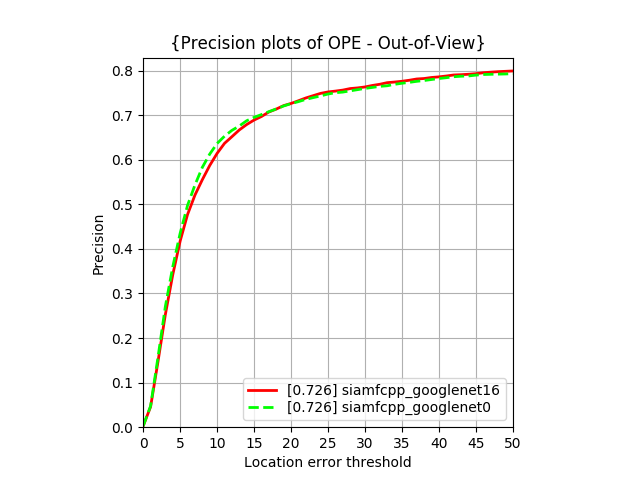
\includegraphics[width=0.33\textwidth]
	{Img/MTP/otb2015/precision_Out-of-View.png}
}
\subfloat[]{
	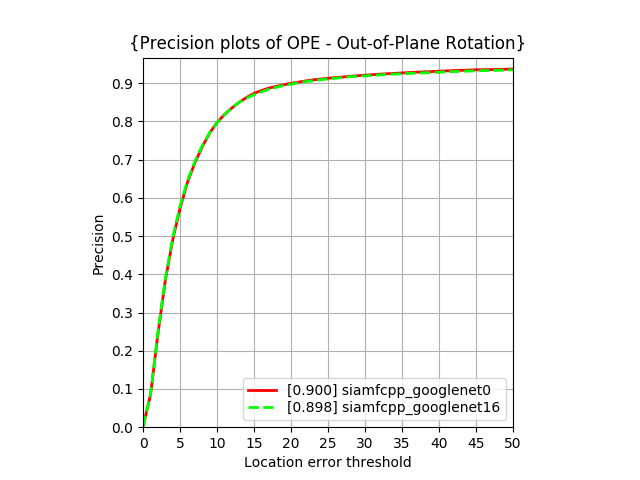
\includegraphics[width=0.33\textwidth]
	{Img/MTP/otb2015/precision_Out-of-Plane Rotation.png}
}\\
\subfloat[]{
	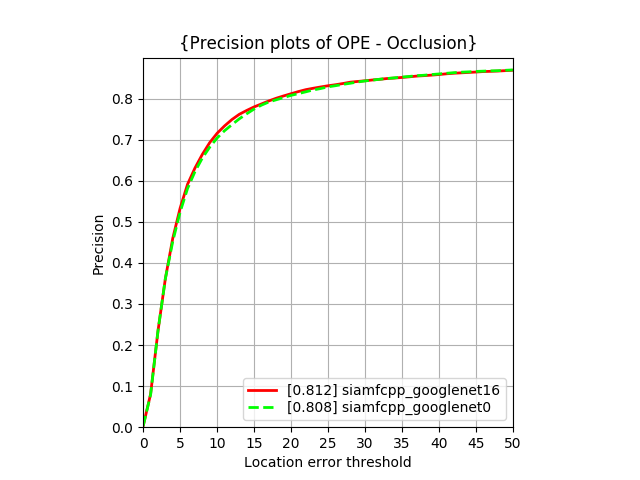
\includegraphics[width=0.33\textwidth]
	{Img/MTP/otb2015/precision_Occlusion.png}
}
\subfloat[]{
	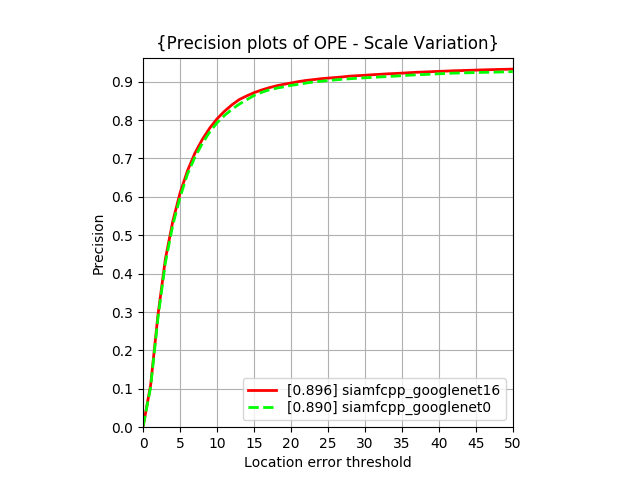
\includegraphics[width=0.33\textwidth]
	{Img/MTP/otb2015/precision_Scale Variation.png}
}
\subfloat[]{
	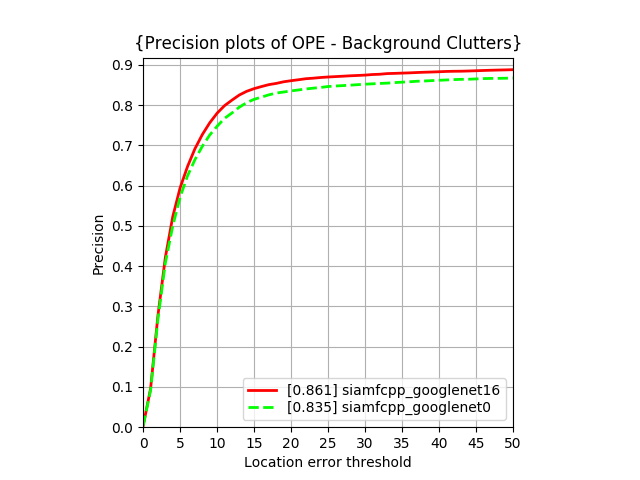
\includegraphics[width=0.33\textwidth]
	{Img/MTP/otb2015/precision_Background Clutters.png}
}\\
\subfloat[]{
	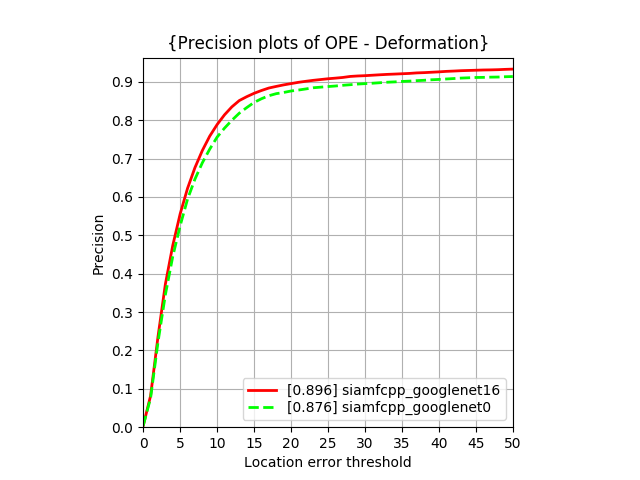
\includegraphics[width=0.33\textwidth]
	{Img/MTP/otb2015/precision_Deformation.png}
}
\subfloat[]{
	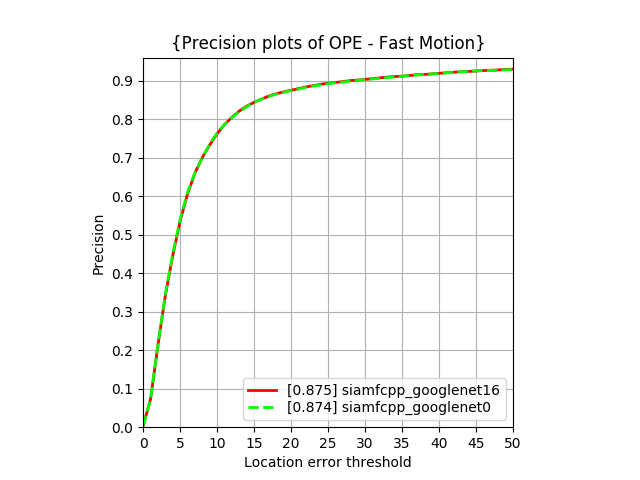
\includegraphics[width=0.33\textwidth]
	{Img/MTP/otb2015/precision_Fast Motion.png}
}
\subfloat[]{
	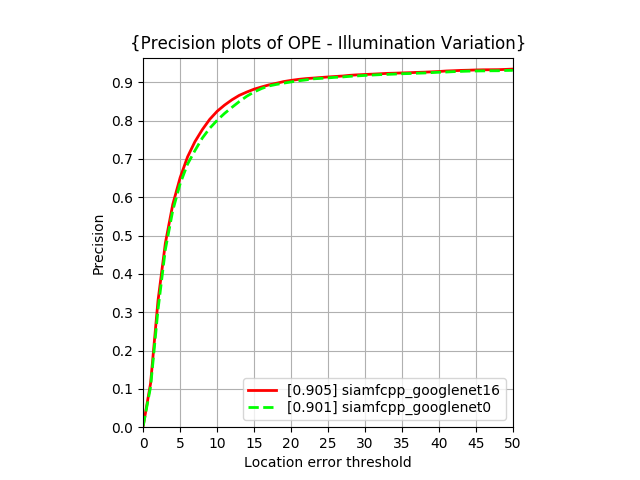
\includegraphics[width=0.33\textwidth]
	{Img/MTP/otb2015/precision_Illumination Variation.png}
}\\
\subfloat[]{
	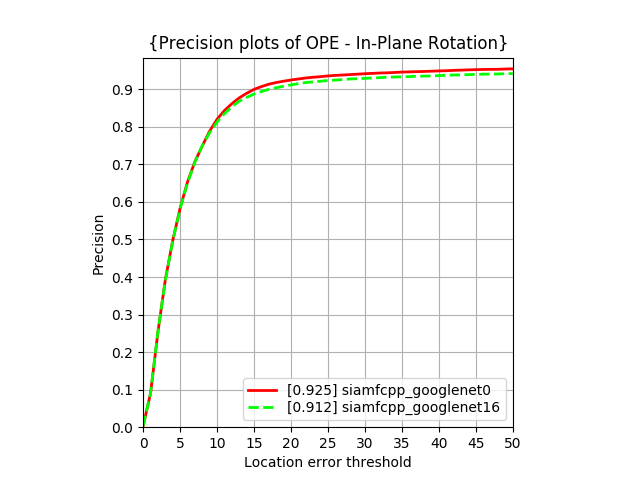
\includegraphics[width=0.33\textwidth]
	{Img/MTP/otb2015/precision_In-Plane Rotation.png}
}
\subfloat[]{
	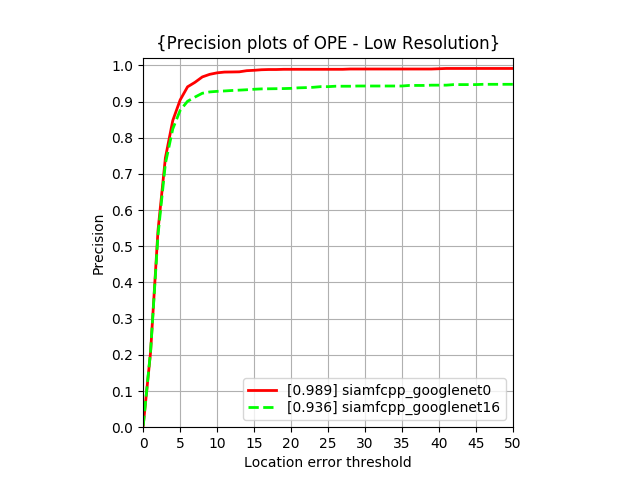
\includegraphics[width=0.33\textwidth]
	{Img/MTP/otb2015/precision_Low Resolution.png}
}
\subfloat[]{
	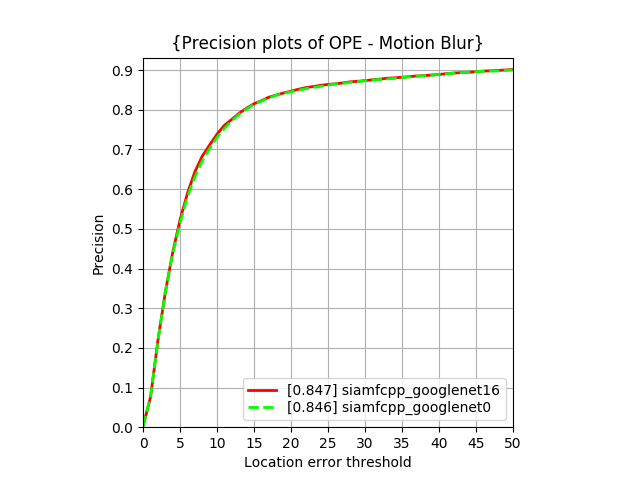
\includegraphics[width=0.33\textwidth]
	{Img/MTP/otb2015/precision_Motion Blur.png}
}
\end{center}
   \caption{OTB 各属性精度图。}
\end{figure*}

\begin{figure*}[p]
\begin{center}
\subfloat[]{
	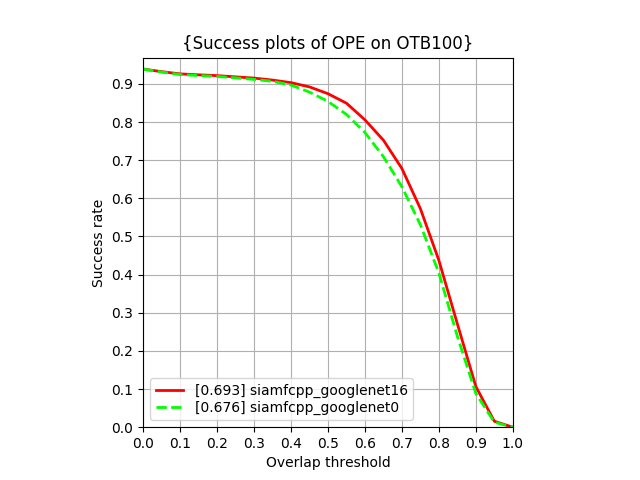
\includegraphics[width=0.33\textwidth]
	{Img/MTP/otb2015/success_ALL.png}
}
\subfloat[]{
	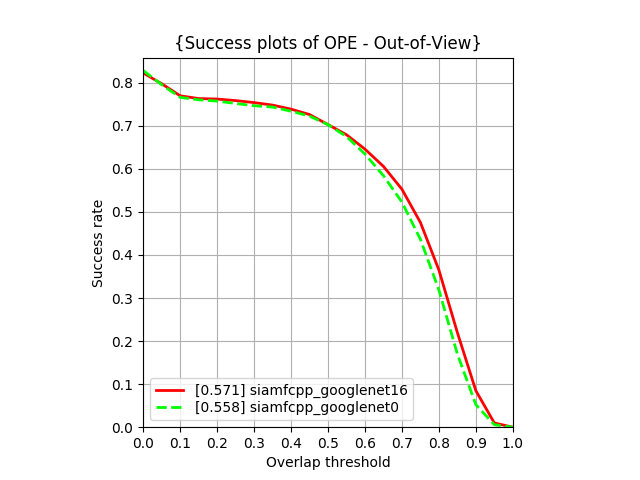
\includegraphics[width=0.33\textwidth]
	{Img/MTP/otb2015/success_Out-of-View.png}
}
\subfloat[]{
	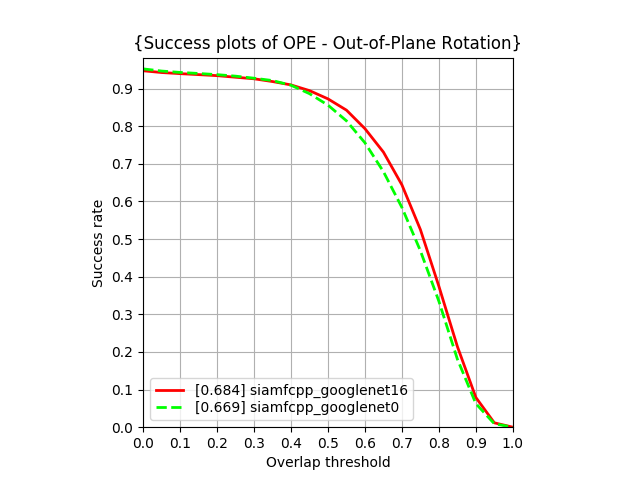
\includegraphics[width=0.33\textwidth]
	{Img/MTP/otb2015/success_Out-of-Plane Rotation.png}
}\\
\subfloat[]{
	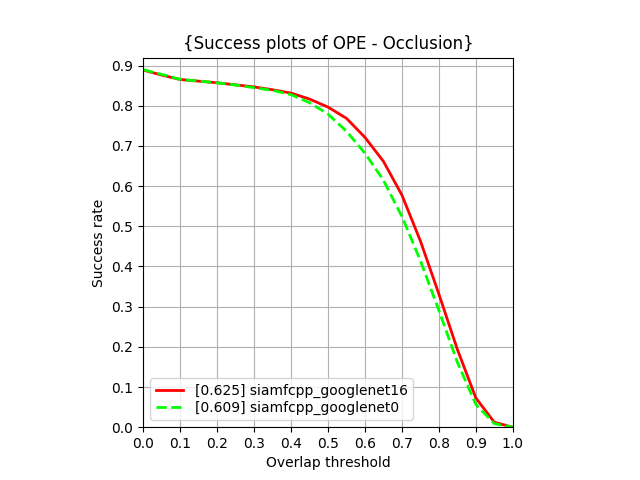
\includegraphics[width=0.33\textwidth]
	{Img/MTP/otb2015/success_Occlusion.png}
}
\subfloat[]{
	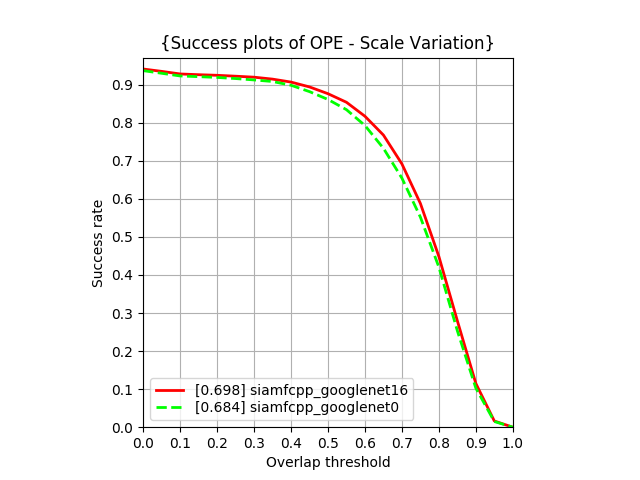
\includegraphics[width=0.33\textwidth]
	{Img/MTP/otb2015/success_Scale Variation.png}
}
\subfloat[]{
	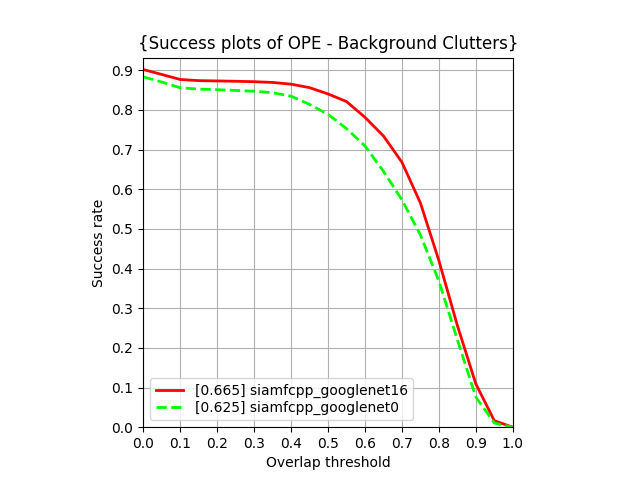
\includegraphics[width=0.33\textwidth]
	{Img/MTP/otb2015/success_Background Clutters.png}
}\\
\subfloat[]{
	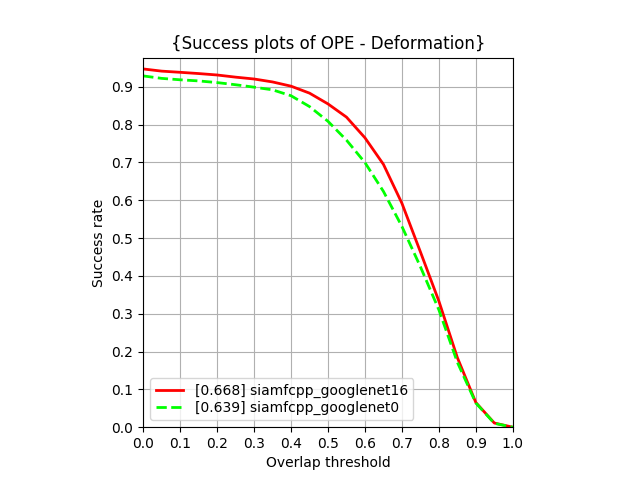
\includegraphics[width=0.33\textwidth]
	{Img/MTP/otb2015/success_Deformation.png}
}
\subfloat[]{
	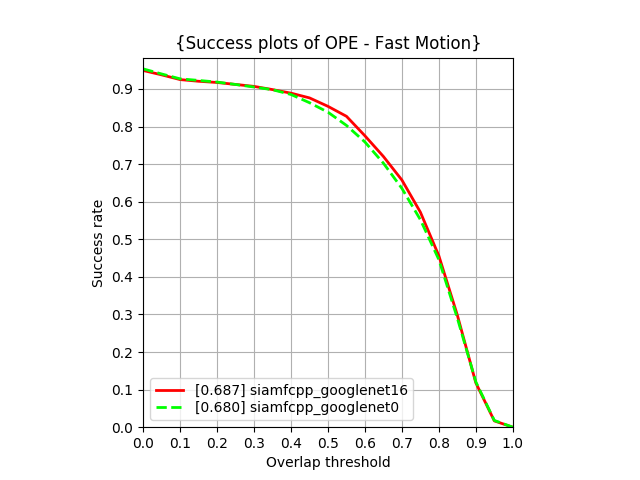
\includegraphics[width=0.33\textwidth]
	{Img/MTP/otb2015/success_Fast Motion.png}
}
\subfloat[]{
	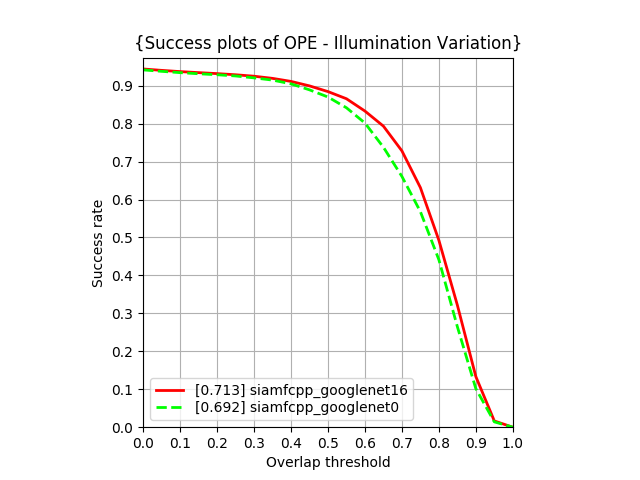
\includegraphics[width=0.33\textwidth]
	{Img/MTP/otb2015/success_Illumination Variation.png}
}\\
\subfloat[]{
	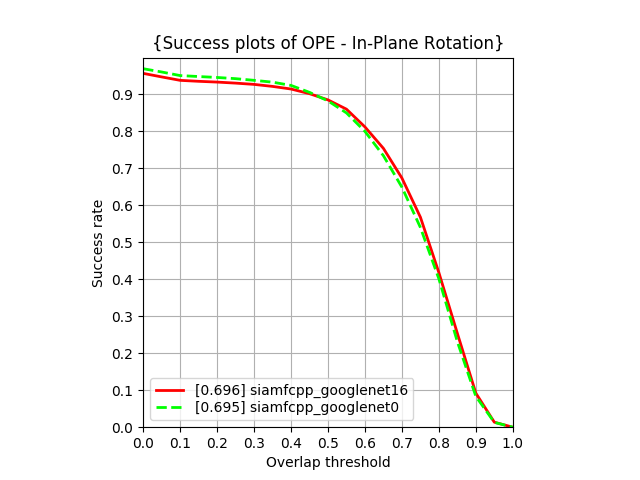
\includegraphics[width=0.33\textwidth]
	{Img/MTP/otb2015/success_In-Plane Rotation.png}
}
\subfloat[]{
	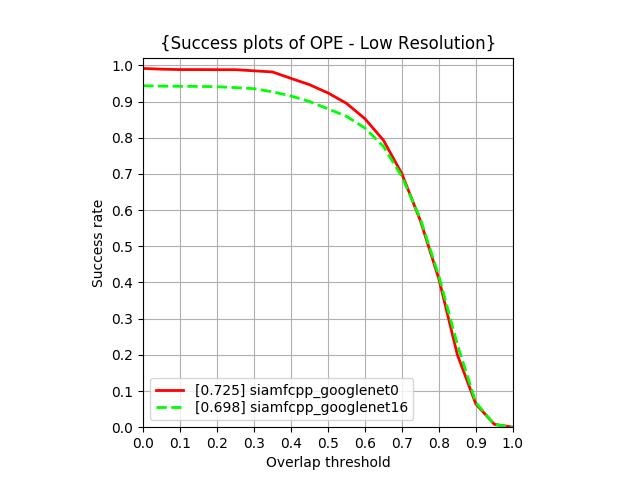
\includegraphics[width=0.33\textwidth]
	{Img/MTP/otb2015/success_Low Resolution.png}
}
\subfloat[]{
	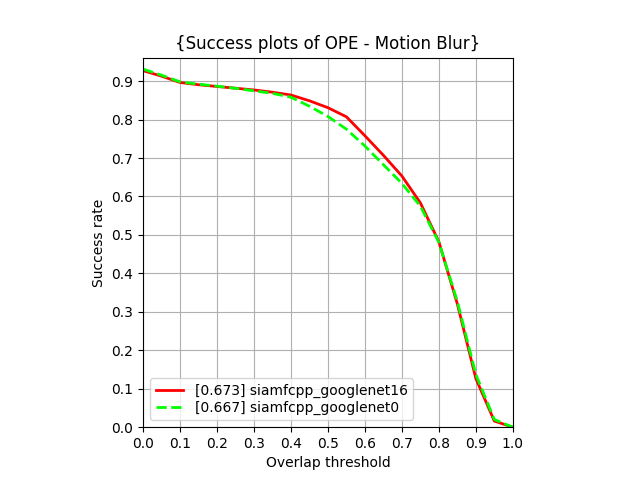
\includegraphics[width=0.33\textwidth]
	{Img/MTP/otb2015/success_Motion Blur.png}
}
\end{center}
   \caption{OTB 各属性成功图。}
\end{figure*}
\fi

\textbf{OTB2015} 我们使用成功率来评估跟踪器在 OTB2015 上的性能。成功率取决于预测边界框和真实边界框的交并比。我们将本章提出的方法与各种跟踪算法进行了比较,包括 ECO \cite{danelljan2017eco},MDNet \cite{MDNet},SiamRPN++ \cite{SiamRPN++},ATOM \cite{danelljan2019atom} 和 SiamFC++\_GoogLeNet \cite{SiamFC++}。模板更新的迭代次数设置为 16。结果显示在表 \ref{table:otb} 中。在成功率方面,我们的跟踪器比在线跟踪器 ATOM 高出 2.8%,这证明了我们方法的强大模型自适应能力。

\textbf{VOT2018} 我们将我们的方法与 RCO \cite{kristan2018sixth},UPDT \cite{bhat2018unveiling},SiamRPN \cite{SiamRPN},MFT \cite{kristan2018sixth},LADCF \cite{kristan2018sixth},ATOM \cite{danelljan2019atom},SiamRPN++ \cite{SiamRPN++},SiamFC++\_AlexNet \cite{SiamFC++} 和 SiamFC++\_GoogLeNet \cite{SiamFC++} 在 VOT2018 上进行了比较。使用鲁棒性和精确度来比较跟踪器。鲁棒性表示跟踪失败的次数,而精确度表示跟踪器预测边界框与真实边界框之间的平均重叠。两种度量方式被合并为单个评价指标——期望平均重叠(EAO)分数。模板更新的迭代次数设置为 2。如图 \ref{fig:eao} 所示,本章提出的跟踪器性能超越了所列出的其他跟踪器。

\textbf{GOT-10k} 我们将平均重叠(AO)分数用作 GOT-10k \cite{GOT-10k} 的性能指标。我们将本章提出的方法与 CF2 \cite{CF2},ECO \cite{danelljan2017eco},CCOT \cite{danelljan2016beyond},GOTURN \cite{GOTURN},SiamFC \cite{SiamFC},SiamFCv2 \cite{valmadre2017end},ATOM \cite{danelljan2019atom},SiamFC++\_AlexNet \cite{SiamFC++} 和 SiamFC++\_Go-
ogLeNet \cite{SiamFC++} 在该数据库上进行比较。模板更新的迭代次数设置为 2。在图 \ref{fig:got10k} 中可以发现,与列出的跟踪器相比,本章提出的算法具有更好的跟踪性能。

\nopagebreak[3]
\begin{table}[t!]
\centering
\caption{本章提出的跟踪算法与相关算法在 TrackingNet \cite{muller2018trackingnet} 测试集上的评测结果。}
\begin{tabular}{l c c c}
\toprule
跟踪器   &  精确度   &  标准化精确度 & 成功率  \\
\midrule
本章算法  &  70.6&  81.7 &74.9 \\
SiamFC++\_GoogLeNet \cite{SiamFC++} & 70.5 & 80.0 & 75.4 \\
SiamFC++\_AlexNet \cite{SiamFC++} & 64.6 & 75.8 & 71.2 \\
ATOM \cite{danelljan2019atom} & 64.8 & 77.1 & 70.3 \\
SiamRPN++ \cite{SiamRPN++} &  69.4 & 80.0 &73.3 \\
MDNet \cite{MDNet} &  56.5&  70.5 &60.6 \\
ECO	\cite{danelljan2017eco} &  49.2&  61.8 &55.4 \\
SiamFC \cite{SiamFC} &  51.8&  65.2 &55.9 \\
\bottomrule
\end{tabular}
\label{tabel:trackingnet}
\end{table}
\nopagebreak[3]


\textbf{TrackingNet} 我们将本章提出的方法与 SiamFC \cite{SiamFC},ECO \cite{danelljan2017eco},MDNet \cite{MDNet},SiamRPN++ \cite{SiamRPN++},ATOM \cite{danelljan2019atom},SiamFC++\_AlexNet \cite{SiamFC++} 和 SiamFC++\_
GoogLeNet \cite{SiamFC++} 进行比较。模板更新的迭代次数设置为 32。表 \ref{tabel:trackingnet} 显示,我们的跟踪器在精确度和标准化精确度方面表现最佳,同时保持了较高的成功率。

\subsection{对初始帧噪声的鲁棒性分析}

%%%%%%%%%%%%%%%
\begin{table}[t]
\centering
\caption{在评测库 OTB2015 上分析初始帧噪声对算法鲁棒性的影响。}
\begin{tabular}{c c c c c}
\toprule
\multicolumn{3}{c}{噪声系数} & \multicolumn{2}{c}{成功率得分} \\
\cmidrule(lr){1-3} \cmidrule(lr){4-5}
$\gamma_1$ & $\gamma_2$ & $\gamma_3$  & SiamFC++\_GoogLeNet \cite{SiamFC++} & 本章算法  \\
\midrule
0.57  &	1.6	 & 0.93	& 67.3    & 69.5 \\
%0.82  & 1.1  & 0.82 & 65.9    & 67.2 \\
0.88  & 0.22 & 0.86 & 65.7    & 68.0 \\
0.88  & 0.43 & 0.77 & 64.1    & 64.4 \\
0.92  & 0.98 & 0.82 & 65.6    & 66.6 \\
0.98  & 0.83 & 0.84 & 66.5    & 67.9 \\
1.0   & 0.81 & 0.79 & 65.3    & 66.0 \\
1.1   &	1.9  & 0.90	& 67.6    & 68.8 \\
1.2   & 0.70 & 0.79 & 65.7    & 66.6 \\
1.3   & 1.3  & 0.77 & 64.9    & 65.8 \\
1.5   & 0.19 & 0.79 & 64.8    & 66.3 \\
1.5   & 1.3  & 0.86 & 66.7    & 68.0 \\
\bottomrule
\end{tabular}
\label{table:noise}
\end{table}
%%%%%%%%%%%

\iffalse
To verify the contribution of the proposed model adaptation method, we compare our tracker with the baseline SiamFC++\_GoogLeNet \cite{SiamFC++} on 4 challenging tracking datasets. In comparison with the baseline tracker on OTB2015, our tracker improves the success score by 1.4\%. On VOT2018, our tracker outperforms the baseline tracker by 1.2\% in terms of EAO. On GOT-10k, our tracker improves the AO score by 1.0\%. On TrackingNet, our tracker outperforms the baseline tracker by 1.7\% in terms of the normalized precision score. All these consistent improvements highlight the effectiveness of the proposed model adaptation method.
\fi

为了研究本章提出的模型自适应方法在初始帧与后续帧相比有噪声的情况下的鲁棒性,我们通过以下方式在第一帧中添加三种噪声:更改图像亮度,应用高斯模糊以及使用不准确的真实边界框注释。我们用 $\gamma_1 \in [0.5, 1.5]$ 表示亮度变化系数,用 $\gamma_2 \in [0, 2]$ 表示模糊半径系数,用 $\gamma_3 \in [0.75, 1]$ 表示不准确的第一帧边界框注释和真实边界框注释之间的边框重叠交并比(IoU)。我们随机采样 $\gamma_1, \gamma_2$ 和 $\gamma_3$,并在 OTB2015 上对基线跟踪器和我们的跟踪器都运行了 10 次(见表 \ref{table:noise})。与 SiamFC++\_GoogLeNet \cite{SiamFC++} 相比,我们的跟踪器在不同的噪声水平下始终表现更好,这表明我们的跟踪器对嘈杂的初始帧具有鲁棒性。%the first frame noise.

\subsection{基于 OTB 数据集不同属性的评测结果分析}
为了对跟踪性能进行进一步分析,我们还通过对 OTB2015 数据集的序列进行基于属性的比较来证明我们算法的优势(请参见表 \ref{table:attr})。在 OTB2015 中,每个序列都具有 11 种不同的属性,即:背景混杂(BC),形变(DEF),快速运动(FM),照明变化(IV),平面内旋转(IPR),低分辨率(LR),运动模糊(MB),遮挡(OCC),平面外旋转(OPR),目标出画面(OV)和缩放尺度变化(SV)。在 11 个属性中,与 SiamFC++\_GoogLeNet \cite{SiamFC++} 相比,本章提出的跟踪器在 10 个属性上具有更好的性能,这证明了其在挑战性跟踪场景(例如照明变化和运动模糊)中的鲁棒性。

%%%%%%%%%%%%%%%%
\begin{table}[t!]
%\renewcommand\arraystretch{0.8}
\centering
\caption{基于评测库 OTB2015 的 11 个属性标注的算法跟踪成功率对比展示。}
\resizebox{\textwidth}{!}{%
\begin{tabular}{c c c c c c c c c c c c}
\toprule
跟踪器 & BC & DEF & FM            & IV            & IPR           & LR    & MB    & OCC   & OPR   & OV    & SV    \\
\midrule
基线算法  &  62.5 & 63.9 & 68.0          & 69.2          & 69.5          & \textbf{72.5}  & 66.7 & 60.9 & 66.9 & 55.8 & 68.4 \\
本章算法        & \textbf{66.5} & \textbf{66.8} & \textbf{68.7} & \textbf{71.3} & \textbf{69.6} & 69.8  & \textbf{67.3} & \textbf{62.5} & \textbf{68.4} & \textbf{57.1} & \textbf{69.8} \\
\bottomrule
\end{tabular}
}
\label{table:attr}
\end{table}
%%%%%%%%%%%

%%%%%%%%%%%%%%%%%%%%
\section{本章小结}
在本章中,我们提出通过操纵模板图像像素以进行自适应信息增强的孪生网络视觉目标跟踪算法,对基于孪生网络的视觉目标跟踪算法在模型初始自适应方面进行改进优化。根据物体第一帧中的损失,对模板图像进行反向传播和微小更新,从而提高对特定物体的自适应能力。我们不仅有效利用了特定物体的表观信息来增强模型的判别能力,而且不修改跟踪算法的模型参数,因此没有模型过拟合的风险。
我们的模型自适应方法是可插拔的,因为它不会改变基线跟踪器的总体架构。
我们在目前比较流行的视频跟踪标准评测库上对通过操纵模板图像像素以进行模型自适应的算法的有效性进行了评估,实验表明该模型自适应方法能够大幅度提升孪生网络跟踪器的性能。
\chapter{空间信息增强的视频目标跟踪算法研究}\label{chap:globally}
在上一章中我们指出,使用语义信息可以增强跟踪器的性能。然而,所提出的语义信息提取网络和目标跟踪网络是单独训练的。最近,孪生网络将特征提取模块和特征匹配模块被设计成一个统一的框架并执行端到端训练,已经取得了出色的跟踪性能。然而,大多数孪生网络跟踪器往往于使用局部搜索机制,目标搜索范围有限,容易造成预测位置的累计误差,从而导致跟踪随时间的漂移。尤其是在长期跟踪情况下,目标频繁进出画面,基于局部搜索机制的孪生网络跟踪器的性能潜力受到较大限制。为了解决这些问题,我们基于 Faster RCNN \cite{ren2015faster} 的两阶段目标检测的思想,提出了一种两阶段孪生网路跟踪器。所提出的跟踪器基于全局感知机制来减少累积误差并提高鲁棒性,该机制可在整个图像平面上感知目标的位置。由于可以在两阶段跟踪框架中使用非常深的网络进行特征学习,因此可以保证特征的判别性。此外,我们还添加了基于卷积神经网络的轨迹预测模块,该模块利用目标的历史运动信息来减轻近似物体的干扰。
本章通过在 GOT-10k \cite{GOT-10k} 和 UAV20L \cite{mueller2016benchmark} 数据集上的大量实验结果,证明了基于空间信息增强的跟踪系统的有效性。

\section{引言}

\begin{figure}[t]
	\centering
    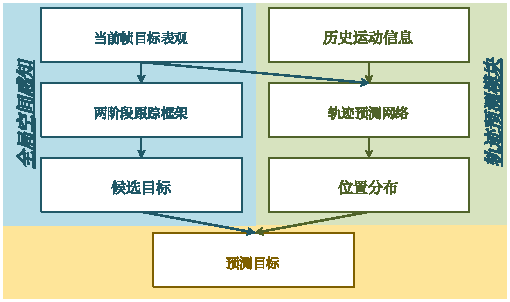
\includegraphics[width=0.8\textwidth]{Img/globally/Arch7.pdf}
    \caption{我们基于全局时空感知(GSTP)的跟踪系统的架构。}
\end{figure}

视频目标跟踪 \cite{Leang2018OnlineFO, Wang2019VisualOT, Zhang2018UsingFL} 是计算机视觉领域中一个具有挑战性的任务,旨在建立连续视频序列中待跟踪目标的位置关系。
流行的孪生网络跟踪器 \cite{SiamFC, SiamRPN, Wang2018SiamMask} 通常基于局部搜索机制:在以前一帧的目标位置为中心的小邻域内搜索目标,从而中确定其在当前帧中的位置。
如果目标仅在两个相邻帧之间具有较小的位移,则此机制可发挥正常作用。该局部搜索机制的另外一个好处是可以避免来自背景中近似物体的干扰。

然而,局部搜索机制存在一些缺点:

\begin{itemize}
\item 首先,如果由于挑战性的照明变化、运动模糊等原因导致先前帧中目标位置的预测偏离了预期,则在当前帧生成的搜索区域可能会无法覆盖真实目标的位置,从而导致不可逆的累积误差,在后续帧彻底跟丢目标。
\item 其次,基于局部搜索机制的跟踪器很难满足长期跟踪的需求 \cite{kalal2011tracking, hong2015multi}。
在长期跟踪情况下,目标经常退出并重新进入画面。
当目标离开画面或重新进入画面时,跟踪器无法设置正确的搜索区域,一旦由于搜索区域设置错误而没有覆盖真实目标的位置,则跟踪器通常无法检索目标。
\end{itemize}

受 Faster RCNN 的两阶段检测框架 \cite{ren2015faster} 的启发,本章提出了一种基于全局感知机制的两阶段孪生网络跟踪器。
在跟踪过程中,所提出的跟踪器始终能够感知整个图像中的目标。
因此,即使跟踪器由于具有挑战性的目标表观变化而犯了一个错误,一旦目标的表观恢复正常,跟踪器便可以及时检索目标。尤其是在长期跟踪中目标离开画面的情况下,当目标从任何位置重新进入画面时,跟踪器便可以继续工作。

所提出的全局感知机制的另一个优势是,跟踪器可以结合 RoI Align \cite{He2018MaskR} 操作,利用更深的网络进行特征学习,而这对于流行的基于局部搜索机制的 SiamFC \cite{SiamFC} 和 SiamRPN \cite{SiamRPN} 跟踪器来说是难以实现的,因为其网络结构中的填充操作将破坏严格的平移不变性 \cite{SiamRPN++},因此尽可以使用浅层神经网络进行特征学习。具体来说,在本章提出的跟踪器中,我们将整个模板图像和搜索图像送入相同的主干网络以提取特征,然后根据初始帧的真实标注信息使用 RoI Align 操作从模板特征中提取目标特征。通过逐通道互相关操作使目标特征和搜索图像特征进行融合,以获得融合特征图,该融合特征图被送入后续的跟踪模块以得到最终的跟踪位置。由于该跟踪框架对平移不变性没有任何限制,因此可以使用具有较强特征提取能力的 ResNet \cite{he2016deep} 作为主干网络来提高跟踪器对前景目标与背景噪声之间的判别性。

除了上述全局空间感知机制外,本章还提出了一种轨迹预测模型来减轻近似物体的干扰,以解决端到端训练的孪生网络跟踪器难以区分表观近似目标的问题。与简单设计的手工策略 \cite{SiamFC, SiamRPN} 不同,本章提出的基于卷积神经网络的轨迹预测模型经过端到端训练,可以使用目标的历史轨迹信息和当前帧中的目标表观信息来预测目标在当前帧中的位置分布。
具体来说,目标的运动模式是在训练阶段从大规模轨迹数据集自动学习的,而不是基于手工制作的特征或规则 \cite{iswanto2017visual};在测试阶段,我们可以使用任意数量的历史帧位置信息,而不是仅基于上一帧的目标位置进行预测。

综上所述,本章做出以下三个主要贡献。
\begin{itemize}
\item 基于全局感知机制,我们引入了一个两步跟踪管道,该管道使用非常深的网络来减少累积误差并提高鲁棒性。
\item 提出了一种新颖的统一的端到端卷积神经网络的轨迹预测结构,利用历史轨迹信息和当前帧的出现信息来预测目标位置分布。
\item 我们在 GOT-10k \cite{GOT-10k} 和UAV20L \cite{mueller2016benchmark} 长期跟踪数据库上优秀的性能证明了我们提出的基于全局时空知觉的跟踪系统(GSTP)的有效性。
\end{itemize}

\iffalse
\section{相关工作之目标跟踪中的运动模型}
在目标跟踪中,运动模型是一个重要的环节。运动模型在目标跟踪中的作用是依据上一帧目标的位置预测在当前帧目标可能出现的区域。在基于孪生网络的目标跟踪中,通常采用静止运动模型。一些工作采用匀加速度运动模型对物体的运动进行建模也带来了性能提升。
\fi

\begin{figure}[t]
    \centering
    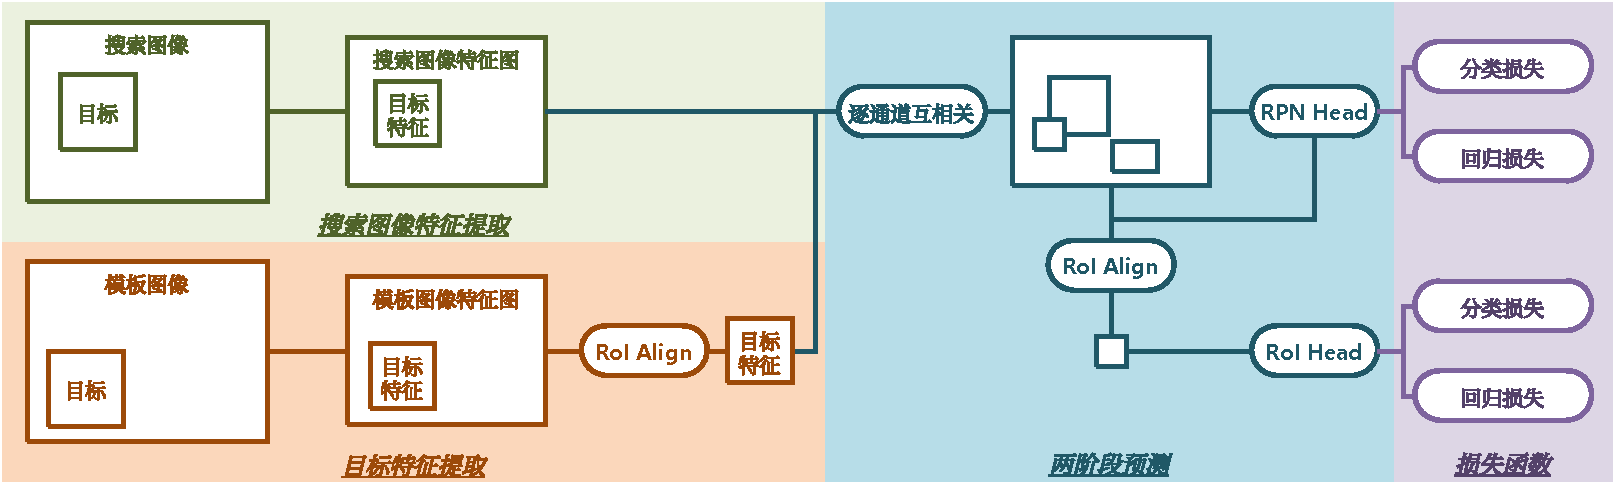
\includegraphics[width=1.0\textwidth]{Img/globally/SiamRCNN.pdf}
    \caption{本章所提算法的网络结构示意图。}
    \label{fig:siamrcnn}
\end{figure}

\section{空间信息增强的视频目标跟踪算法}

\iffalse
\begin{figure*}
    \centering
    \includegraphics[width=12cm]{images/NetworkStructure1.pdf}
    \caption{The proposed tracking framework.}
    \label{fig:network}
\end{figure*}
\fi

\iffalse
\begin{figure*}
    \centering
    \includegraphics[width=12cm]{images/MotionModel.pdf}
    \caption{The effect of the motion model. SiamRCNN detects the real target (in green box) and the distractor (in red box). The motion model predicts the position distribution measuring the likelihood that the target is located at each spatial location. The motion model eliminates the distractor and preserves the real target.}
    \label{fig:motion_model}
\end{figure*}
\fi

在本章中,我们采用如下步骤进行视频目标跟踪任务:首先基于全局感知机制提取候选目标区域,然后使用轨迹预测模块消除近似物体的干扰。通过采用该跟踪流程,我们可以通过设计更精确的候选目标提取模块和更鲁棒的的轨迹预测模型共同提升孪生网络的目标跟踪性能,尤其是长期目标跟踪性能。

总体而言,本章提出了空间信息增强的全局感知系统具有如下贡献:
\begin{itemize}
\item 我们使用整个图像而不是小的图像块作为跟踪器的输入,以为跟踪器提供更丰富的全局空间信息。
\item 为了更好地感知全局空间信息,本章提出了一个两阶段跟踪框架,该框架能够检测在视觉表观上类似于真实目标的候选目标区域。
\item 为了消除候选目标区域中近似物体的干扰,本章提出了一个轨迹预测模块,该模块能够通过预测目标在当前帧的位置分布以排除近似物体,获得最终的跟踪结果。
\end{itemize}

\iffalse
Most state-of-the-art trackers adopt a one-stage framework, which performs classification and bounding box regression only once based on features obtained by cross-correlation.
In the field of object detection, the performance of two-stage detectors is usually better than that of one-stage detectors.
Inspired by this, we design our tracker as a two-stage network.
The RPN stage rapidly filters out most background samples, and the RoI head adopts a fixed foreground-to-background ratio to maintain a manageable balance between foreground and background.
In addition, two steps of regressions achieve accurate localization even for objects with extreme shapes.
\fi

\begin{figure}[t]
\centering
    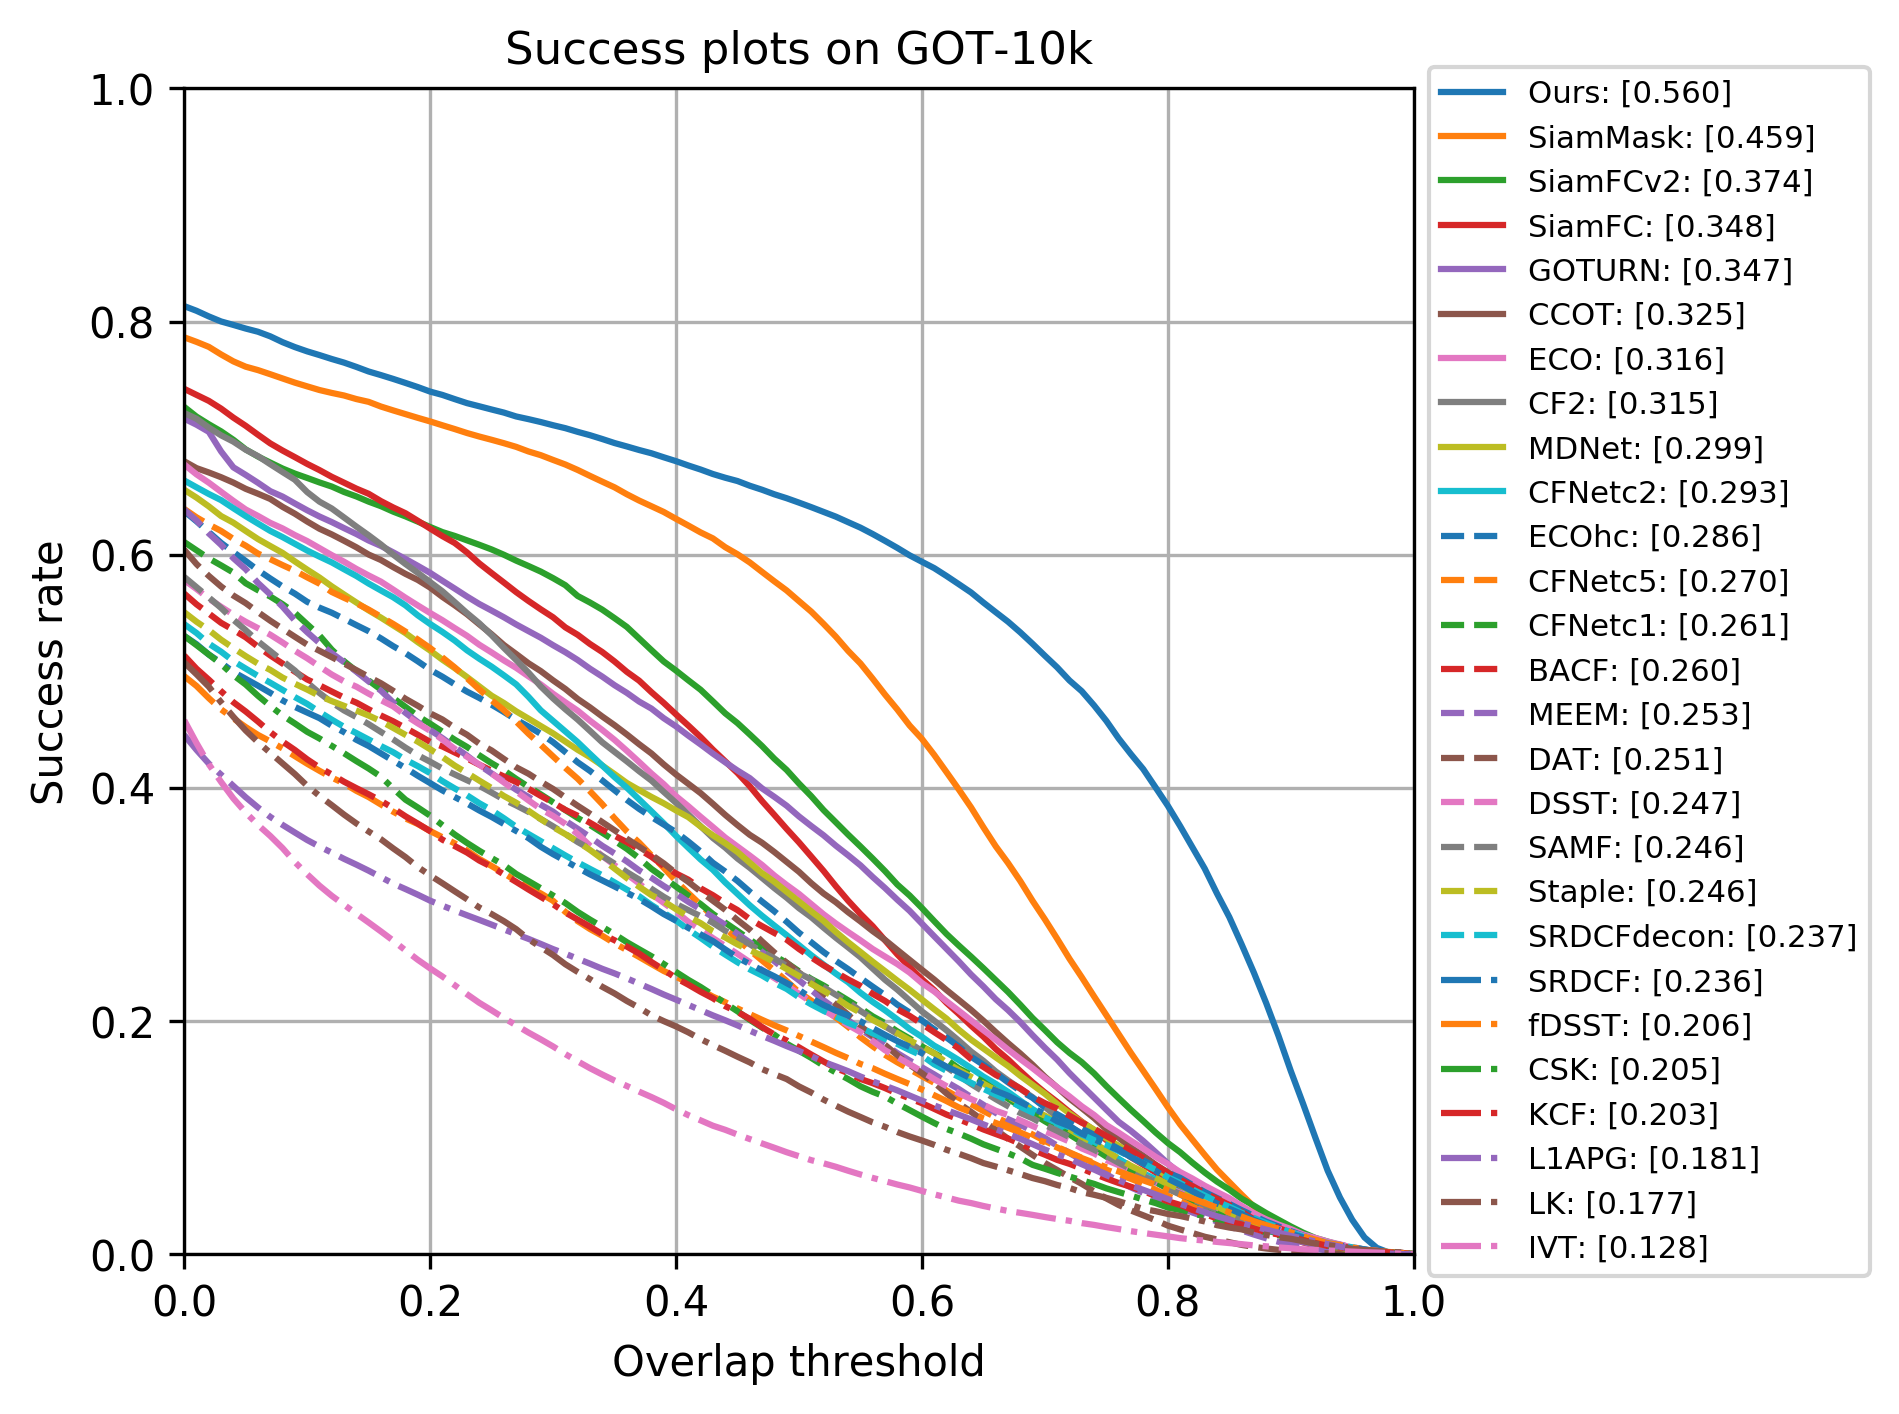
\includegraphics[width=0.75\textwidth]{Img/globally/success_plot.png}
    \caption{GOT-10k 的总体性能,按平均重叠(AO)得分进行排名。}
\end{figure}

\subsection{两阶段跟踪框架}

我们基于流行的目标检测架构 Faster RCNN \cite{ren2015faster} 来构建跟踪框架。尽管利用目标检测模块和孪生网络进行视频目标跟踪并非在本章中首次提出,但本章提出的视频目标跟踪算法与类似视频目标跟踪方法 \cite{SiamRPN, Wang2018SiamMask, danelljan2019atom, voigtlaender2019siam} 相比具有优势。与 SiamRPN \cite{SiamRPN}相比,SiamRPN 的网络输入始终是目标位于中心的图像块,而本章提出的跟踪算法的输入是整个图像,这意味着目标可能出现在图像中的任何空间位置。这防止了网络学习到偏向中心位置的错误先验,从而打破了空间不变性约束 \cite{SiamRPN++} 对于网络体系结构设计的限制。因此,可以采用非常深的卷积神经网络(例如ResNet50 \cite{he2016deep})用于跟踪算法的特征提取器。有关空间不变性玉树和中心位置偏差的详细说明,请参考 \cite{SiamRPN++}。
%because the input of the network is the entire image, instead of the image patch centered on the target, the target will appear in any poisition in the image, so we do not need the network has strict spatial invariance restriction \cite{SiamRPN++}, so we can use a deeper feature extractor, i.e., resnet50. 
与 SiamRPN \cite{SiamRPN} 和 SiamMask \cite{Wang2018SiamMask} 相比,本章提出的跟踪算法采用两阶段体系结构。第二阶段(RoI head \cite{ren2015faster})可以更有效地区分前景和背景。
与 SiamMask \cite{Wang2018SiamMask} 和 ATOM \cite{danelljan2019atom} 相比,本章的跟踪器可以在整个图像中搜索目标,从而在由于遮挡、运动模糊等原因导致跟踪结果出错后,仍可在目标表观恢复正常时重新跟踪目标。
与 Siam R-CNN \cite{voigtlaender2019siam} 相比,Siam R-CNN 的特征提取网络和 RPN 的网络参数是冻结的,未针对视频目标跟踪任务进行端到端训练,而本章提出的跟踪器中,特征提取网络可以生成特定于目标的特征,并且可以端到端地训练整个网络。在视频目标跟踪中,一个视频中的前景目标可能是另一个视频中的背景噪声。因此,本章跟踪器中的 RPN 模块生成的候选目标区域可以更好地满足通用目标跟踪的需求。

\begin{figure}[t]
\begin{minipage}{0.48\linewidth}
  \centering
  \centerline{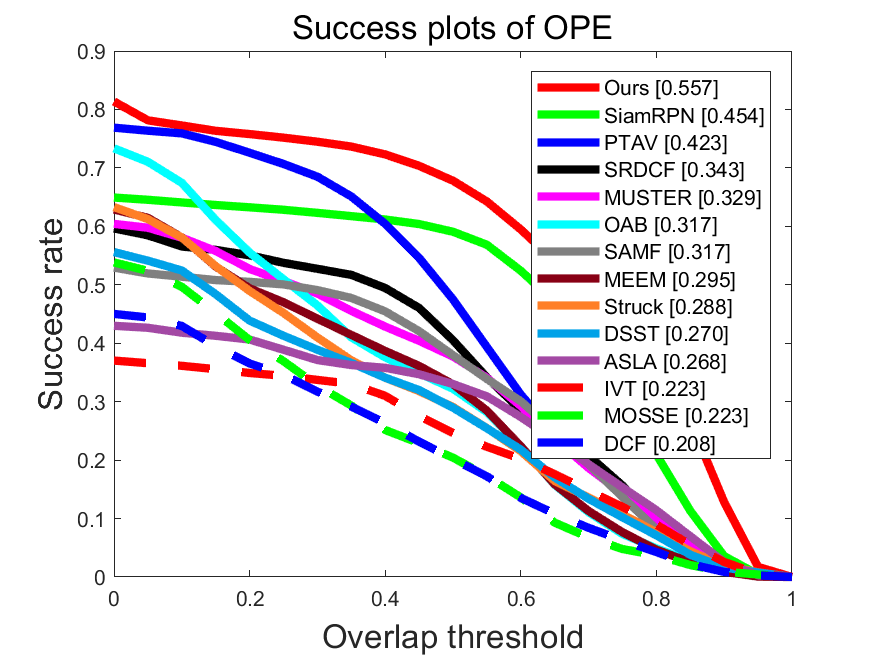
\includegraphics[width=1.0\textwidth]{Img/globally/UAV20L/quality_plot_overlap_OPE_AUC.png}}
\end{minipage}
\hfill
\begin{minipage}{0.48\linewidth}
  \centering
  \centerline{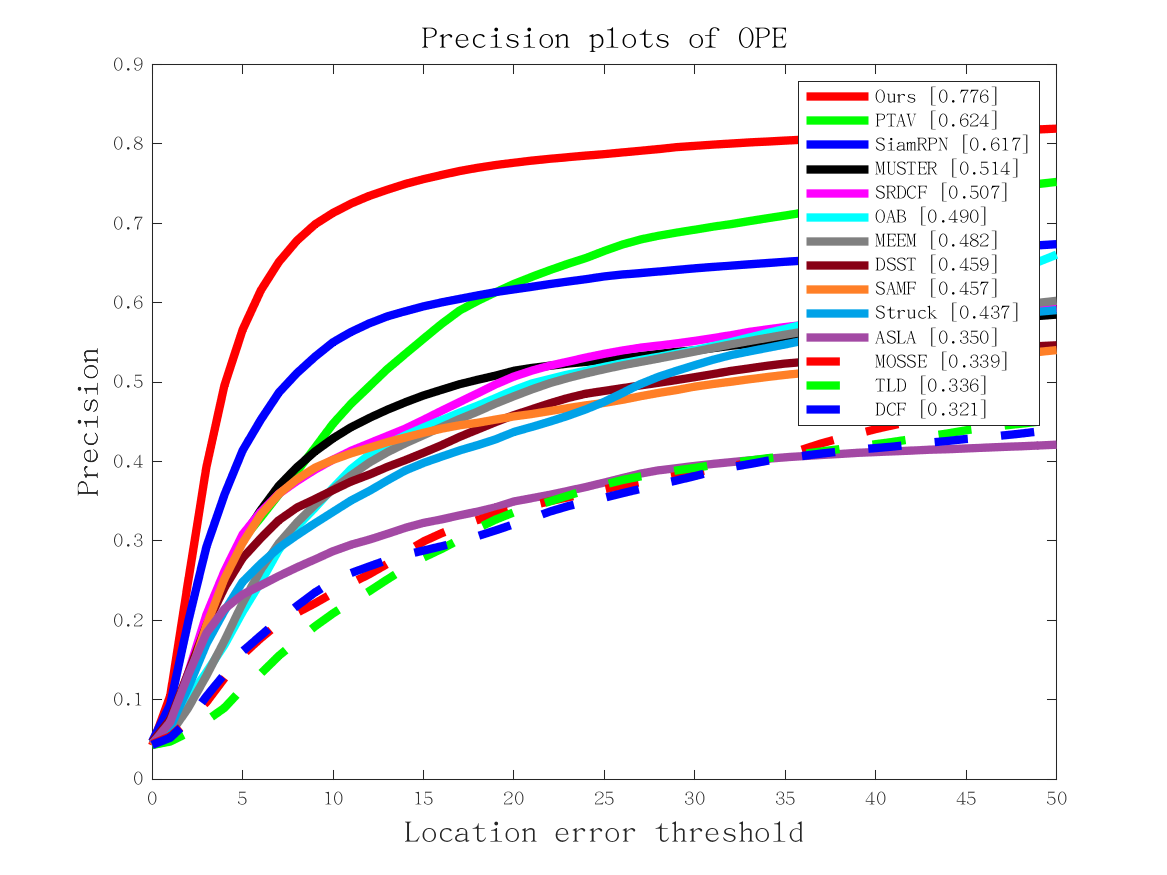
\includegraphics[width=1.0\textwidth]{Img/globally/UAV20L/quality_plot_error_OPE_threshold.png}}
\end{minipage}
\caption{UAV20L 数据集上的成功图和精度图。}
\label{fig:globally_uav20l}
\end{figure}

%(The backbone and RPN are frozen and only the redetection head (after concatenation) is trained for tracking) they fixed the parameters in the backbone and the RPN. Only the second stage is used for target spercific tracking, which is not good for "generatic" object tracking: because some objects are foreground in some cases and background in others. Instead, our tracker use the correlation before RPN, the "target" which is good for general object tracking. The architecture of our tracking component is described as follows:

%The first component of our tracking framework (i.e., SiamRCNN) is a two-stage tracker (Fig. \ref{fig:siamrcnn}) used to detect object regions that are visually similar to the given first-frame template object.
%Specifically, the tracking component consists of four modules: (1) feature extraction module, (2) feature fusion module, (3) RPN head module, and (4) RoI head module.

%The transplant from a detection task to a tracking task using faster RCNN is straightforward and easy to implement.
%, which is another advantage of our tracking module. 
为了描述本章提出的跟踪框架,我们首先简要回顾一下 Faster RCNN。该目标检测网络包括一个特征提取器,其后是两个检测模块:RPN 头和 RoI 头。
特征提取器 $\phi_{1}$ 是 ResNet50 的变体。第一阶段使用区域生成网络(RPN)在特征提取网络的最后一个特征图上执行滑动窗口操作,在判断每个空间位置是否存在目标的同时,预测这些目标的边界框。
在第二阶段(即 RoI head)中,区域生成网络生成的每个候选区域,利用 RoI Align \cite{He2018MaskR} 操作提取尺度相同的深度特征
使用分类层将每个候选区域(region of interest,ROI)分类为特定类别,并使用回归层对边界框位置进行进一步微调。请参阅 \cite{ren2015faster} 了解更多详细信息。

对于目标跟踪任务,特征提取器 $\phi_{1}$ 有两个输入:模板图像 $z$ 和搜索图像 $x$。根据孪生架构的设计,两个输入共享相同的网络参数以提取特征。
在生成模板特征 $f_{z} = \phi_{1}(z)$ 和搜索特征 $f_{x} = \phi_{1}(x)$ 之后,利用 RoI Align 操作 \cite{He2018MaskR},根据目标的真实标注框,模板特征中裁剪得到目标特征 $f_{obj} \in \mathbb{R}^{1024 \times 7 \times 7}$:
\begin{equation}
    f_{obj} = \mathcal{R}(b_{obj}, f_{z}),
\end{equation}
其中 $\mathcal{R}$ 表示 RoI Align 运算符,而 $b_{obj}$ 是目标的真实边界框。
接下来,通过逐通道互相关 \cite{SiamRPN++} 操作融合搜索特征和目标特征:
\begin{equation}
    f_{corr} = f_{obj} * f_{x},
\end{equation}
其中 $f_{corr}$ 是融合特征,$*$ 是逐通道互相关算子。
%The use of RPN (region proposal network) is ...
然后将 $f_{corr}$ 发送到 RPN head 以生成候选目标 $B=\{b^{i}_{roi}\}^{i=1:N}$。
\iffalse
There are two inputs to the feature extraction module: the template image $z$ and the search image $x$. According to the design of the siamese architecture, the two inputs share the same network parameters to extract features.
The network structure of the feature extraction module is a variant of ResNet50, which is pretrained on the 1000-class ImageNet classification set. Features of the input images are extracted from the final convolution layer of the 4-th stage. The obtained template features $f_{z} = \phi(z)$ and search features $f_{x} = \phi(x)$ with channel dimension 1024 and stride 16 are sent to the subsequent feature fusion module.

In the feature fusion module, object features $f_{obj}$ are obtained by the RoI Align operation from the template features according to the ground truth of the target. The search features and the object features are merged via the depth-wise cross-correlation:
\begin{equation}
    f_{obj} = \mathcal{R}(b_{obj}, f_{z})
\end{equation}
where $\mathcal{R}$ represents the RoIAlign, $\odot$ represents the element-wise multiplication, $b$ represents an RoI in candidate proposals and $\mathcal{X}$ represents the fused feature of $b$.
\begin{equation}
    f_{corr} = f_{obj} * f_{x}.
\end{equation}
Two 1 $\times$ 1 convolutions with channel dimension 1024 are added on top of the correlation layer to obtain the fusion feature.

The RPN head includes two sibling 1 $\times$ 1 convolutional layers -- a classification layer with channel dimension 2$k$, and a regression layer with channel dimension 4$k$, where $k$ is the number of maximum possible proposals for each location. The RPN head takes the fusion feature as input and simultaneously regress region bounds and objectness scores for each anchor.
\fi
%The RoI head is run for each region proposed by the RPN by performing RoI Align \cite{He2018MaskR} to extract deep features from this proposed region.
在第二阶段,对融合特征 $f_{corr}$ 执行 RoI Align 操作,为每个 RoI 生成一个小特征图,其通道尺寸为 2048,空间分辨率固定为 7 $\times$ 7:
\begin{equation}
    f_{roi}^{i} = \mathcal{R}(b_{roi}^{i}, f_{corr}),
\end{equation}
其中 $b_{roi}^{i}$ 是候选区域 $i$ 的边界框。
最后,每个 RoI 被分类为前景或背景。在测试期间,我们选择排名靠前的 $K$ 的 RoI 作为候选目标,这些目标将在轨迹预测模块中进行后处理。

\iffalse
The RoI Aligned features are fed into the global average pooling layer followed by two sibling output layers: one that produces softmax probability estimates over two classes (foreground or background) and another layer that outputs four real-valued numbers for the foreground class. These four values encode the refined bounding-box position for the RoI.
The loss of SiamRCNN is:
$$Loss = L_{cls}^{rpn} + L_{cls}^{roi} + \lambda (L_{reg}^{rpn}+L_{reg}^{roi}),$$
where $\lambda$ is hyper-parameter to balance the classification loss and the regression loss. $L_{cls}^{*}$
is the cross entropy loss and $L_{reg}^{*}$ is the standard smooth $L1$ loss for regression.
\fi

\begin{table}[t]
\centering
\caption{本章提出的算法在 GOT-10k 测试集上,不同组件的性能。}
\begin{tabular}{c c c c c}
\bottomrule
ROI head & Motion model & $AO$ & $SR_{0.50}$ & $SR_{0.75}$ \\ 
\hline
          &           & 0.410 & 0.486 & 0.162 \\
\checkmark&           & 0.521 & 0.595 & 0.440 \\
\checkmark&\checkmark & 0.560 & 0.645 & 0.457 \\
\bottomrule
\label{table:globally_ablition}
\end{tabular}
\end{table}

\subsection{轨迹预测模块}
使用前文提出的的跟踪框架提取到与给定的第一帧模板目标在视觉表观上相似的候选目标区域后,我们利用轨迹预测模块消除近似物体的干扰并获得最终的跟踪结果。
轨迹预测模块以端到端的方式,使用目标的历史轨迹信息和当前帧的表观信息学习目标位置分布,该目标位置分布是一个二维热图,用于度量目标位于每个空间位置的可能性,我们根据该目标位置分布信息重新评估每个候选目标。

\begin{table}[t]
\centering
\caption{将本章提出的方法与其他视频目标跟踪方法在 GOT-10k 测试集上的跟踪结果进行比较。跟踪器按其平均重叠(AO)分数排名。}
\begin{tabular}{l l l l}
\bottomrule
Method   &  $AO$   &  $SR_{0.50}$ & $SR_{0.75}$  \\
\hline
Ours &  $\textbf{0.560}^\textbf{1}$ & $\textbf{0.645}^\textbf{1}$  & $\textbf{0.457}^\textbf{1}$  \\
SiamMask &  0.459&  0.560 &0.205 \\
SiamFCv2 &  0.374&  0.404 &0.144 \\
SiamFC   &  0.348&  0.353 &0.098 \\
GOTURN	 &  0.347&  0.375 &0.124 \\
CCOT	 &  0.325&  0.328 &0.107 \\
ECO	     &  0.316&  0.309 &0.111 \\
CF2	     &  0.315&  0.297 &0.088 \\
MDNet	 &  0.299&  0.303 &0.099 \\
CFNetc2	 &  0.293&  0.265 &0.087 \\
ECOhc	 &  0.286&  0.276 &0.096 \\
\bottomrule
\end{tabular}
\label{table:got}
\end{table}

令 $H_{t}^{k} = \{h_{t-i}\}_{i=1:k}$ 表示历史轨迹信息,其中 $t$ 是当前帧的索引,$k$ 是历史长度,并且 $h_{j} = \{x_{j}, y_{j}\}$ 是一个二维坐标,表示目标在帧 $j$ 中的位置。
受姿态估计任务的启发,我们将 $h_{j}$ 表示为二维热图 $m_{j} \in \mathbb R^{h \times w}$,其中二维高斯顶点位于目标位置 $(x_{j}, y_{j})$。
为了对目标的轨迹信息进行建模,我们根据时间顺序将生成的 $k$ 热图进行串接,以获得通道维度为 $k$ 的轨迹张量 $\mathcal{M} \in \mathbb{R}^{k \times h \times w}$:
\begin{equation}
    \mathcal{M}_{t}^{k} = \mathcal{C}(m_{t-k}, m_{t-k+1}, ..., m_{t-1}),
\end{equation}
其中 $\mathcal{C}(\cdot)$ 表示串联操作。

本章提出的轨迹预测模块不仅利用历史轨迹信息进行预测,同时页考虑当前帧的表观信息。
为此,将当前帧 $\mathcal{I} \in \mathbb{R}^{3 \times h \times w}$ 的 RGB 图像与轨迹张量串接起来,以获得增强的轨迹张量 $\mathcal{N} \in \mathbb{R}^{(3+k) \times h \times w}$,通道尺寸为 $(3+k)$:
\begin{equation}
    \mathcal{N}_{t}^{k} = \mathcal{C}(\mathcal{I}_{t}, \mathcal{M}_{t}^{k}).
\end{equation}
假设 $\phi_{2}$ 是基于卷积神经网络的轨迹预测模型,则 $\phi_{2}$ 的输出计算如下:
\begin{equation}
    \mathcal{O}_{t}^{k} = \phi_{2}(\mathcal{N}_{t}^{k}),
\end{equation}
其中 $\mathcal{O}_{t}^{k} \in \mathbb{R}^{h \times w}$ 是二维热图,它反映了目标在 $t$ 帧中的位置分布。

本章提出的运动模型 $\phi_{2}$ 的网络与姿势估计网络 HRNet \cite{sun2019deep} 相同。
\iffalse
The main reason why the pose estimation network can be used to design the motion model is that the output of the pose estimation network is the position distribution of joint points, and the output of the motion model is the position distribution of the target. This means that there is a great deal of commonality between the two tasks. In order to use HRNet for trajectory estimation, we need to change the input and output of HRNet and keep the network structure unchanged.

During tracking the $i$-th frame, we utilize the position information of the previous $K$ frames as the input to the network.
Specifically, for a historical frame, a heat map is generated by applying 2D Gaussian with stand deviation of 3 pixels centered on the target position in that frame.
The generated $K$ heatmaps are concatenated according to the time order to obtain the \textbf{trajectory tensor} with channel dimension $K$.
Our motion model not only utilizes the historical trajectory information for prediction, but also considers the appearance information of the current frame.
To achieve this, the RGB image of the current frame and the trajectory tensor are concatenated to obtain the tensor with channel dimension $(3+K)$. This tensor is sent to the network, and the output of the network is a heatmap reflecting the position distribution of the target in the current frame. The loss function, defined as the mean squared error, is applied for comparing the predicted heatmap and the groundtruth heatmap. The groundtruth heatmap is generated by applying 2D Gaussian with standard deviation of 3 pixels centered on the target position in the current frame. The network structure of our motion model is the same as HRNet. 
\fi
这里提供简要说明。HRNet 的第一阶段是高分辨率子网。在此基础上依次添加从高分辨率到低分辨率的子网,以形成更多的阶段。多分辨率子网之间并行连接。通过在整个网络中重复地在并行多分辨率子网中交换信息来进行多尺度融合。我们利用 HRNet 的高分辨率输出来表示目标的位置分布。有关网络结构的详细信息,请参考 \cite{sun2019deep}。

\begin{table}[t]
\centering
\caption{从 GOT-10k 验证集中收集的具有不同属性子集的性能。}
\begin{tabular}{|c|c|c|c|c|c|c|}
\hline
\multirow{2}{*}{属性} &
\multicolumn{2}{c|}{SiamFC} & \multicolumn{2}{c|}{SiamMask} &\multicolumn{2}{c|}{本章方法} \\
\cline{2-7} & $AO$ & $SR_{0.5}$ & $AO$ & $SR_{0.5}$ & $AO$ & $SR_{0.5}$ \\
\hline
快速运动 & 0.472 & 0.538 & 0.526 & 0.608 & 0.639 & 0.715 \\
\hline
遮挡 & 0.411 & 0.447 & 0.494 & 0.559 & 0.585 & 0.659 \\
\hline
图像边界切割 & 0.505 & 0.545 & 0.595 & 0.701 & 0.738 & 0.837 \\
\hline
长视频 & 0.557 & 0.655 & 0.643 & 0.779 & 0.721 & 0.807 \\
\hline
\end{tabular}
\label{table:attribute}
\end{table}

\section{实验结果与分析}

\subsection{实验设置}

\begin{figure*}[t!]
\begin{center}
	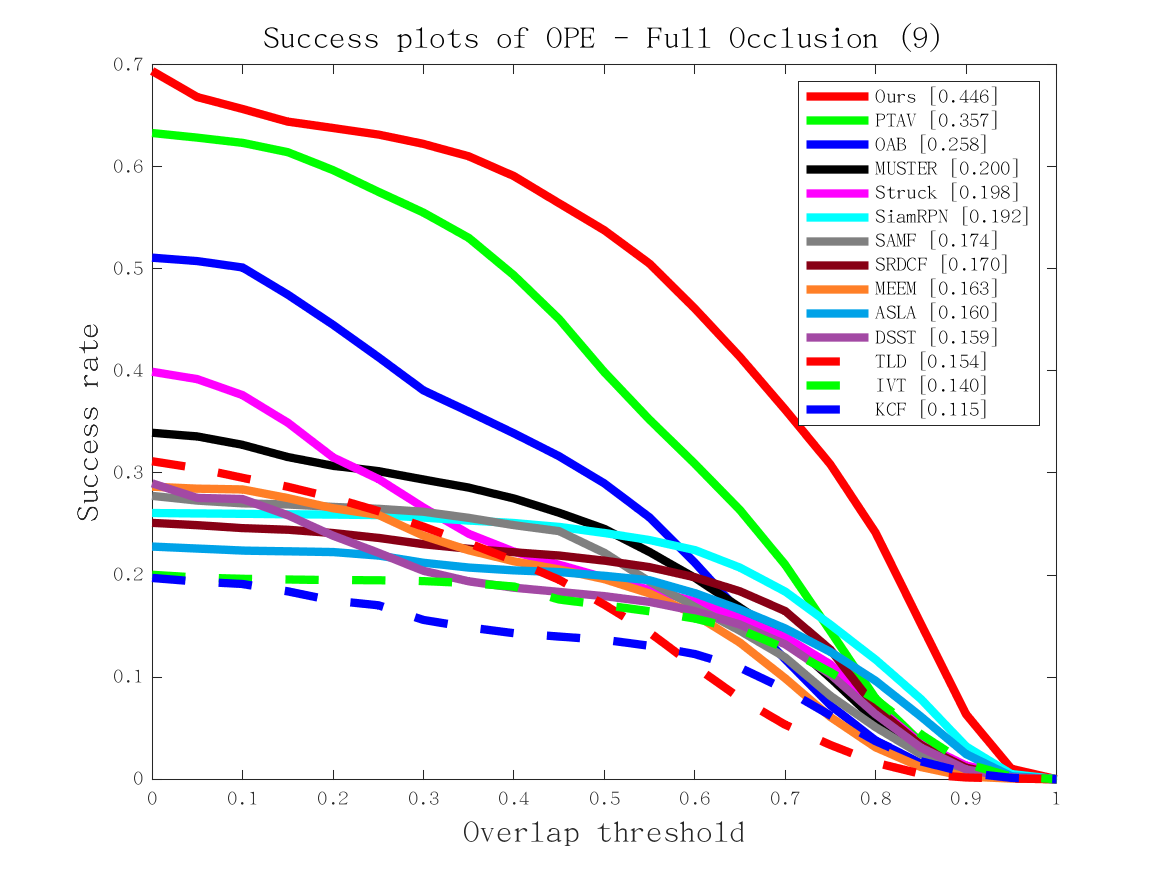
\includegraphics[width=0.48\textwidth]{Img/globally/UAV20L/FOC_overlap_OPE_AUC.png}
	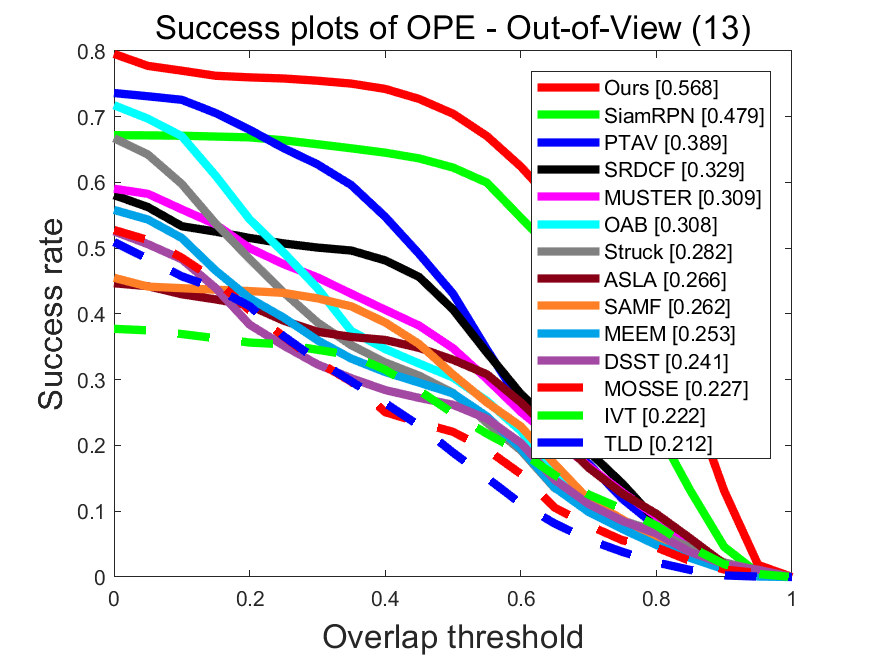
\includegraphics[width=0.48\textwidth]{Img/globally/UAV20L/OV_overlap_OPE_AUC.png}
	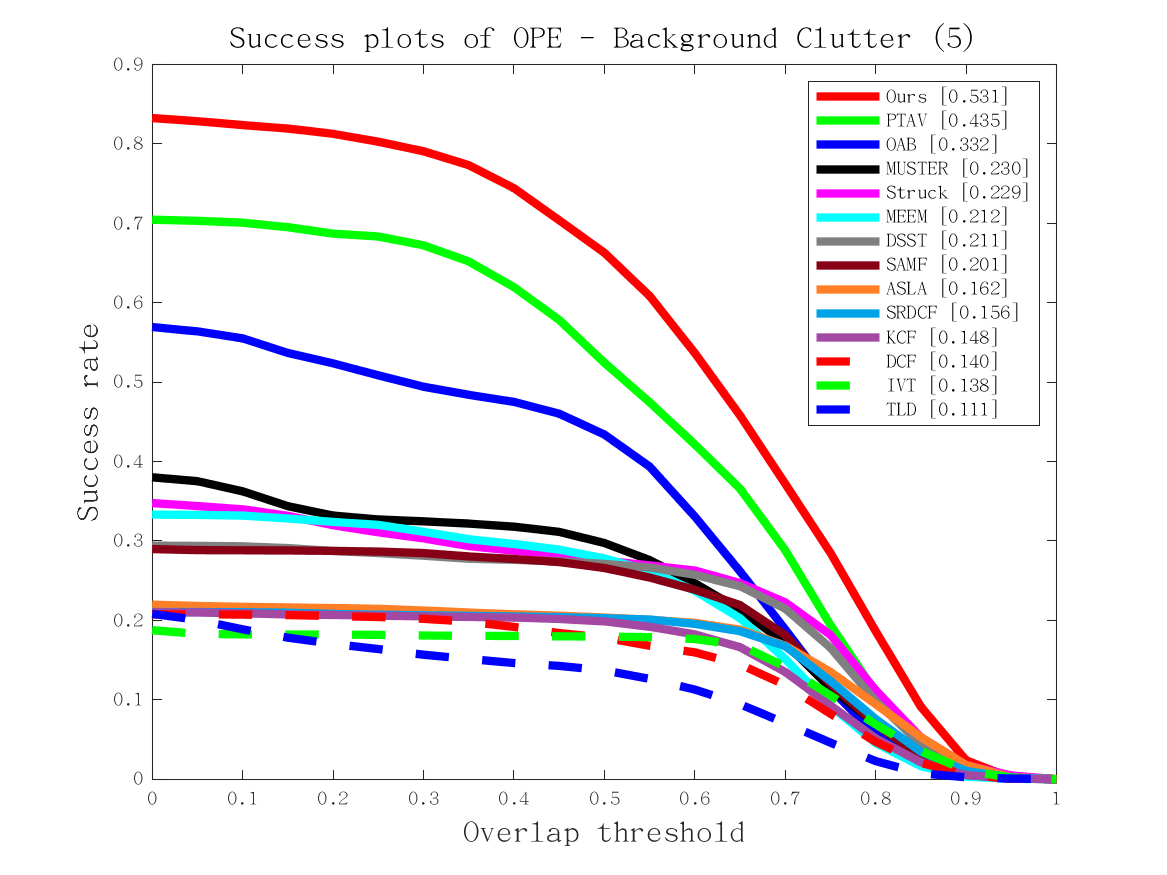
\includegraphics[width=0.48\textwidth]{Img/globally/UAV20L/BC_overlap_OPE_AUC.png}
	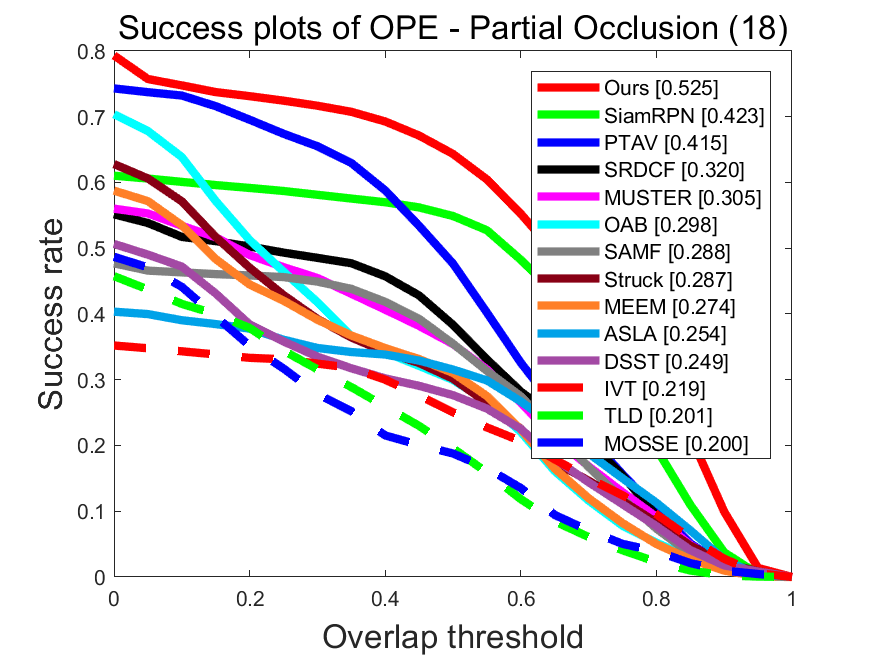
\includegraphics[width=0.48\textwidth]{Img/globally/UAV20L/POC_overlap_OPE_AUC.png}
	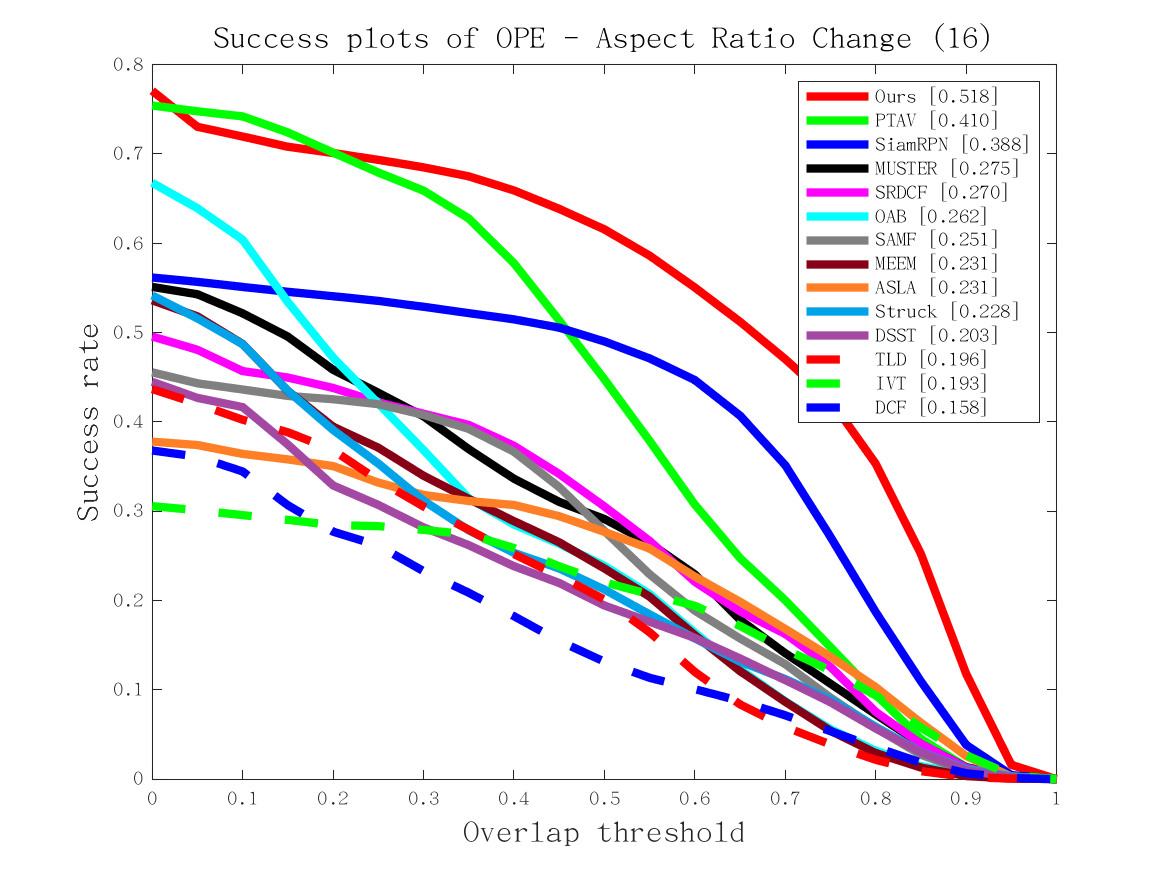
\includegraphics[width=0.48\textwidth]{Img/globally/UAV20L/ARC_overlap_OPE_AUC.png}
	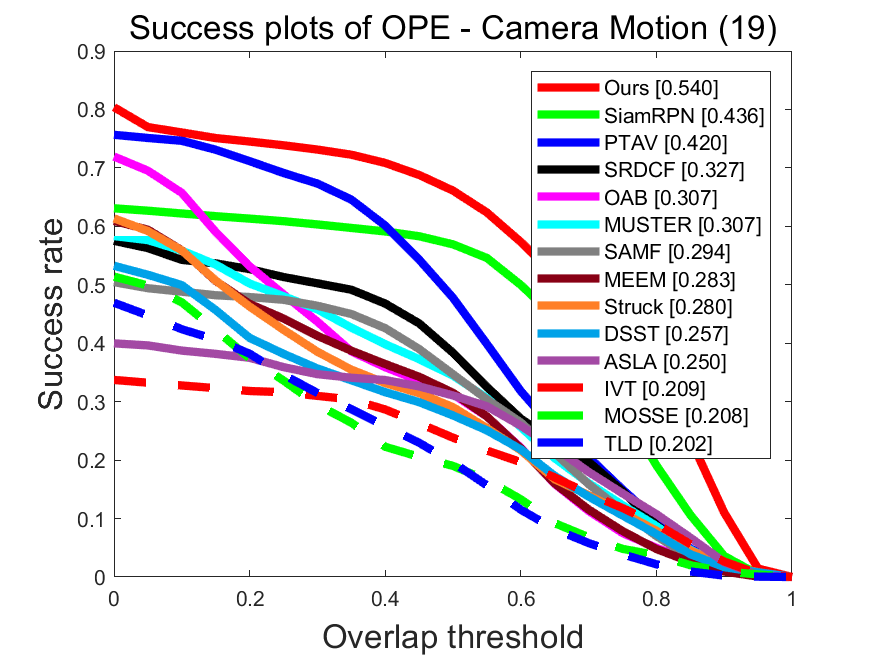
\includegraphics[width=0.48\textwidth]{Img/globally/UAV20L/CM_overlap_OPE_AUC.png}
\end{center}
   \caption{在 UAV20L 上成功绘制带有属性的图 1。在彩色显示屏上观看效果最佳。}
\label{fig:globally_uav20l_1}
\end{figure*}

\textbf{网络架构设计}:本章提出的空间信息增强的孪生视频目标跟踪网络主要有三个子网络组成,分别是用于共享特征提取的主干网络、用于生成特定目标特征的特征调制子网络以及用于边框微调的区域细化子网络。它们的网络结构如图 \ref{fig:siamrcnn} 所示,主干网络基于 ResNet-50 设计,可以为模板图像和搜索区域图像提取深度特征,以提升特征表示能力。

\textbf{训练数据}:为了提高特征表示的泛化能力和判别能力,同时避免在稀缺的跟踪数据上过拟合,离线训练过程在大规模单目标视频跟踪数据库 GOT-10k \cite{GOT-10k} 的训练数据集中训练网络参数。GOT-10k 数据集具有超过 10000 个真实运动目标的视频片段和超过 150 万个手动标记的边界框,包括 563 类真实运动目标和 87 类运动模式。
我们执行多尺度训练:目标大小从 $64 \times 64$ 至 $256 \times 256$ 不等。图像大小在跟踪过程中保持不变。

\textbf{优化器参数设定}:本章使用动量为 0.9 的随机梯度下降(stochastic gradient descent,SGD)优化器从在 ImageNet 上预训练的网络参数开始训练,并将权值衰减参数设置为 $10^{-4}$。学习率从 $10^{-2}$ 指数衰减到 $10^{-4}$。该模型经过 27000 次迭代训练,每个批次大小为 2 个样本对。

本章提出的轨迹预测模块也利用 GOT-10k 训练集进行训练。训练采用的优化器为 Adam 优化器 \cite{kingma2014adam}。初始学习率设置为 $10^{-3}$,并在第 170 轮和 200 轮迭代时分别降至 $10^{-4}$ 和 $10^{-5}$。训练过程在 210 轮迭代后终止。

本章所提出的时间信息增强的孪生网络跟踪器使用 Pytorch 在 Python 中实现,所有实验在装配有 Intel(R) Xeon(R) CPU E5-2630 v4 @ 2.20GHz 和 NVIDIA TITAN 1080Ti GPU 的工作站上执行。

\subsection{对 GOT-10k 数据集的评估}
在本节中,我们在 GOT-10k \cite{GOT-10k} 数据集上评估所提出的跟踪算法。
GOT-10k 的评价指标包括平均重叠(AO)和成功率(SR)。AO 表示所有真实边界框和预测边界框之间重叠的平均值,而 SR 表示重叠超过 0.5/0.75 的成功进行跟踪的帧占总帧数的百分比。

\textbf{对比实验}
为了分析本章提出的两阶段跟踪框架和轨迹预测模块的有效性,我们训练了两个跟踪网络的变体。变体 1(参见表 \ref{table:globally_ablition} 第一行)在我们最终提出的跟踪器中同时剔除了 RoI 头和轨迹预测模块。变体 2(参见表 \ref{table:globally_ablition} 第二行)在我们最终提出的跟踪器中剔除轨迹预测模块,仅保留 RoI 头。表 \ref{table:globally_ablition} 的第三行表示我们最终提出的跟踪器,同时配备有 RoI 头和轨迹预测模块。
我们在 GOT-10k 测试集上对上述三个跟踪器的性能进行了对比。
从第一行和第二行中可以看出,通过添加 RoI 头,AO 性能提高了 11.1%。这是因为 RPN 阶段可快速过滤掉大多数背景样本,并且 RoI 头采用固定的前景与背景比率,以在前景与背景之间保持可控的样本平衡。
第二行和第三行中可以看出,通过添加轨迹预测模块,AO、SR$_{0.50}$ 和 SR$_{0.75}$ 分别增加 3.9\%,5.0\% 和 1.7\%。这是因为所提出的轨迹预测模块可以有效地预测目标的位置分布,从而避免了近似物体的不利干扰。

\begin{figure*}[t!]
\begin{center}
	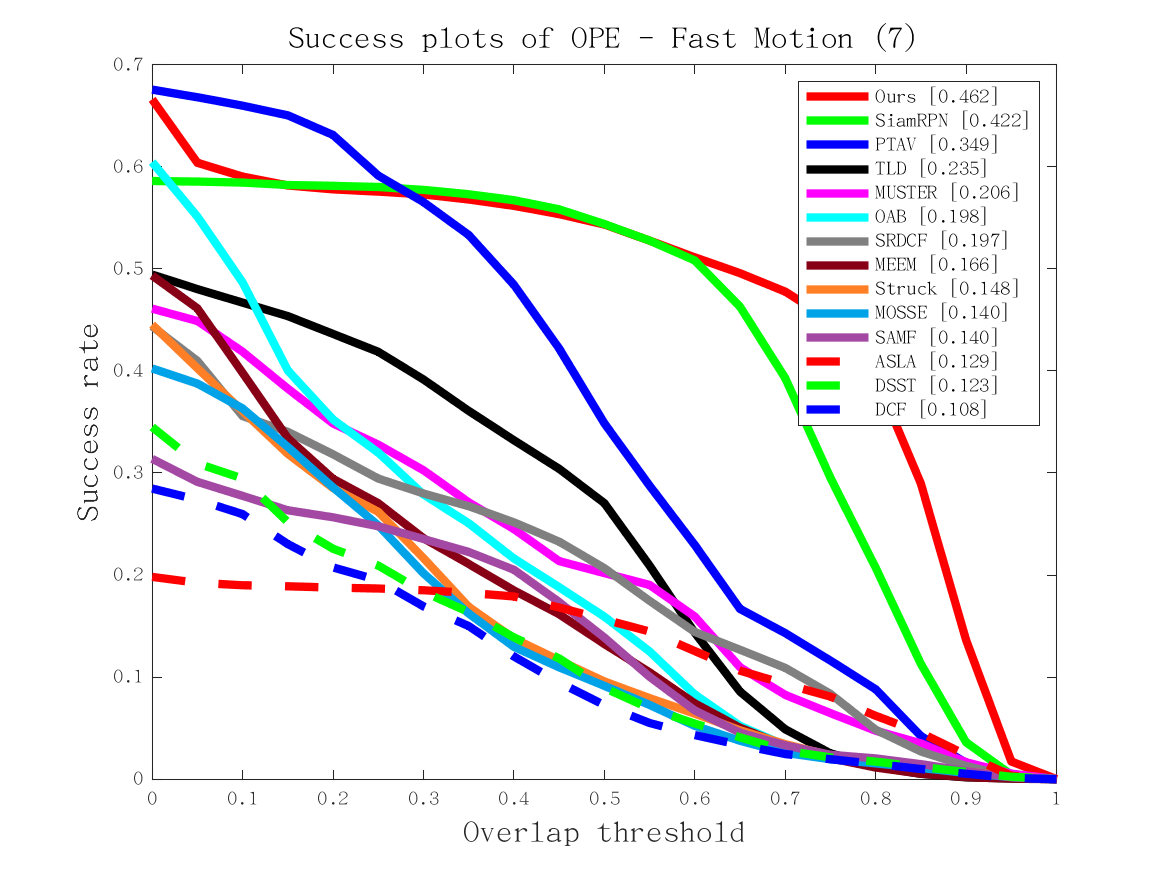
\includegraphics[width=0.48\textwidth]{Img/globally/UAV20L/FM_overlap_OPE_AUC.png}
	\includegraphics[width=0.48\textwidth]{Img/globally/UAV20L/IV_overlap_OPE_AUC.png}
	\includegraphics[width=0.48\textwidth]{Img/globally/UAV20L/LR_overlap_OPE_AUC.png}
	\includegraphics[width=0.48\textwidth]{Img/globally/UAV20L/SOB_overlap_OPE_AUC.png}
	\includegraphics[width=0.48\textwidth]{Img/globally/UAV20L/SV_overlap_OPE_AUC.png}
	\includegraphics[width=0.48\textwidth]{Img/globally/UAV20L/VC_overlap_OPE_AUC.png}
\end{center}
   \caption{在 UAV20L 上成功绘制带有属性的图 2。在彩色显示屏上观看效果最佳。}
\label{fig:globally_uav20l_2}
\end{figure*}

\nopagebreak[3]
\begin{figure}[p!]
    \centering
    \includegraphics[width=0.9\textwidth]{Img/globally/visulization.pdf}
    \caption{本章提出的跟踪器与主流跟踪器 SiamMask \cite{Wang2018SiamMask} 和SiamFCv2\cite{SiamFC} 的比较。示例帧来自 GOT-10k \cite{GOT-10k} 测试集。}
    \label{fig:gloablly_vis}
\end{figure}
\nopagebreak[3]

\textbf{总体效果}
我们在 GOT-10k 测试集上将本章提出的方法与 8 个跟踪器(包括最新提出的跟踪器)进行了比较。
与列出的方法相比,我们的方法实现了 0.560 的 AO 得分(表 \ref{table:got})。
CSK 是基于 DCF 的典型跟踪器之一,它使用有效的循环矩阵理论导出闭式解,并使用使用几种类型的核进行训练和跟踪。相反,本章提出的跟踪器基于特征提取能力更强的卷积神经网络。因此,本章提出的跟踪器在 AO 得分方面远超 CSK,相对提升为 173.17%,这证明了卷积神经网络出色的特征表示能力以及本章提出的算法的有效性。
MDNet 具有多个分支,可学习共享层和特定域的层,其中不同的域对应不同的训练序列,每个分支负责二进制分类以识别每个域中的目标。相比之下,本章提出的跟踪器通过对目标模板和搜索区域的特征表示进行互相关操作来学习通用相似度特征图。与 MDNet 相比,本章提出的跟踪器的 AO 得分相对提升为 87.29%,这表明孪生架构和互相关运算在视频跟踪任务中的有效性。
SiamMask 是最新的跟踪器之一,它是一个孪生跟踪器,并可利用非常深的卷积神经网络进行提取特征。SiamMask 利用区域生成子网来预测目标的位置。
与 SiamMask \cite{Wang2018SiamMask} 相比,本章提出的两阶段跟踪器是基于全局感知机制设计的,可以减少跟踪过程中的累积误差,另外,轨迹预测模块可抑制近似物体的干扰并提高跟踪的鲁棒性。因此,本章提出的跟踪器在 AO 方面的性能要比 SiamMask 高出 22.00%,体现了所提出的两阶段跟踪框架和轨迹预测模块的有效性。

\textbf{按属性进行的性能分析}
GOT-10k 训练/验证数据集中的每个视频都带有多个属性,包括:目标可见率、运动速度、视频长度和按图像边界切割。为了分析跟踪器在不同属性下的性能,我们将跟踪器与两个最新的跟踪器(即 SiamFC  \cite{SiamFC} 和 SiamMask \cite{Wang2018SiamMask})在 GOT-10k 验证集上进行了比较。我们根据属性注释从验证集中收集四个子集:FM(快速运动)子集,OC(遮挡)子集,CU(图像边界切割)子集和 LO(长视频)子集。
FM 子集包括目标运动速度很快的视频。
OC 子集包括目标经常被遮挡的视频。
CU 子集包括目标经常被图像边界切割的视频。
LO 子集包括验证集中最长的 40 段视频。
表 \ref{table:attribute} 展示了跟踪算法的不同属性下的性能。
在 FM 子集上,本章提出的方法在 AO 方面的表现优于 SiamMask \cite{Wang2018SiamMask},相对提升为 21.48\%。
%This result suggests that our motion model is capable of modeling challenging motion patterns.
在 AO 方面,本章提出的算法在 OC 和 CU 子集上的性能分别比 SiamMask 高 18.42% 和 24.03%。
%This result suggests that our two-stage tracker based on ResNet50 is able to handle the appearance changes caused by heavy occlusion.
在 LO 子集上,与 SiamMask 相比,AO 得分的相对提升为 12.13%。结果表明,全局感知机制可以有效减少视频目标跟踪算法在跟踪长视频时的累积误差。

\subsection{对 UAV20L 数据集的评估}

UAV20L \cite{mueller2016benchmark} 是从低空鸟瞰视角捕获的航拍视频数据集。UAV20L 数据库专为长期跟踪而设计,包含 20 个视频,平均长度为 2934 帧。
遵循 OTB50 \cite{OTB} 的评估方法,我们使用精确度和成功率来评估 UAV20L 数据集上跟踪器的性能。精确度反映了指从预测边界框的中心点到真实边界框的中心点的距离。成功使用预测边界框与真实边界框的边框重叠计算得到。在图 \ref{fig:globally_uav20l} 中,不同跟踪器的性能比较通过精度图和成功图进行可视化。

我们将本章提出的方法与 13 个主流跟踪器进行了比较。图 \ref{fig:globally_uav20l} 清楚地表明,本章提出的算法在成功率和精确度得分方面均由于所提出的其他跟踪器。具体来说,在成功图中,我们的跟踪器获得的 AUC 得分为 0.557。与主流方法 PTAV \cite{fan2018parallel} 和 SiamRPN \cite{SiamRPN} 相比,本章提出的跟踪器的相对 AUC 提升分别为 31.7% 和 22.7%。在精度图中,本章所提算法的得分为 0.776。与 SiamRPN \cite{SiamRPN} 和 PTAV \cite{fan2018parallel} 相比,本章所提出的跟踪器的相对性能提升分别为 25.8\% 和 24.4\%。

此外,我们对 UAV20L 进行了基于属性的分析(参见图 \ref{fig:globally_uav20l_1} 和图 \ref{fig:globally_uav20l_2})。UAV20L 包含常见的视觉跟踪挑战,包括宽高比变化(aspect ration change,ARC)、背景混杂(background clutter,BC)、相机运动(camera motion,CM)、快速运动(fast motion,FM)、完全遮挡(Full Occlusion,FOC)、光照变化(illumination variation,IV)、低分辨率(low resolution,LR)、视线外(out-of-view,OV)、部分遮挡(partial occlusion,POC)、相似目标(similar object,SOB)、尺度变化(scale variation,SV)和视点改变(viewpoint change,VC)。
与所列出的方法相比,本章提出的方法在所有属性下均取得了最好的跟踪结果。
在文献 \cite{SiamRPN} 中,Li 等人提出了同时具有分类分支和回归分支的跟踪框架 SiamRPN。分类分支旨在在搜索图像中确定目标的位置,回归分支旨在优化目标的边框尺寸与长宽比。通过两个分支的合作,SiamRPN 具有较高的跟踪性能。因此,该算法在尺度变化、视点改变等属性上得分较高。尽管如此,SiamRPN 与本文提出的算法仍具有较大差距。比如在完全遮挡属性中,SiamRPN 的成功率仅为 0.192,而本章提出的算法成功率为 0.446。可能的原因是 SiamRPN 基于局部搜索机制进行跟踪,而本章提出的跟踪器采用了全局感知机制和轨迹预测模块,能够在目标再次出现在画面后及时进行继续跟踪。

\iffalse
In order to perform a more in-depth and detailed analysis of the performance of the trackers, we also report the results on challenging attributes in UAV20L. Fig. \ref{fig:uav20l_attr} lists the success plots of 14 different methods on 12 attributes: ARC (Aspect Ratio Change), BC (Background Clutter), CM (Camera Motion), FM (Fast Motion), FOC (Full Occlusion), IV (Illumination Variation), LR (LR Low Resolution), OV (Out-of-View), POC (Partial Occlusion), SOB (Similar Object), SV (Scale Variation) and VC (Viewpoint Change). We can observe that the AUC of the proposed algorithm perform better than other methods on most challenging attributes, which means our method is more robust than other approaches on various difficult situations.
\fi
\section{本章小结}
在本章中,我们提出了一种空间信息增强的视频目标跟踪算法,其中包括基于全局感知机制的两阶段跟踪框架和数据驱动的轨迹预测模块。全局感知机制允许跟踪组件减少跟踪过程中的累积误差。跟踪框架使用非常深的网络进行两阶段跟踪,使跟踪器提取的特征更具判别性。轨迹预测模块通过端到端训练,能够从大规模轨迹数据集中学习目标的运动模式。通过基于全局感知机制的两阶段跟踪框架和轨迹预测模块的协同工作,本章所提出的方法可实现较好的跟踪性能。
\chapter{语义信息引导的视觉目标跟踪算法研究}\label{chap:IGCF}

对于视觉目标跟踪算法而言,判别表观学习具有极其重要的地位。在缺少目标类别先验的情况下,跟踪任意类别的目标通常需要在线进行目标前景与背景的判别信息学习,同时目标大小、形状、视角以及背景场景中光照、遮挡物、嘈杂干扰等都会随着时间发生剧烈变化。
基于传统相关滤波器(correlation filter,CF)的跟踪器通常仅依靠岭回归进行表观模型的建模,而不会感知目标在语义级别的信息。这种语义信息的缺乏可能导致跟踪漂移或跟踪器完全失效。为了解决这一问题,本章提出了实例引导的相关滤波器(instance guided correlation filter,IGCF),以提高跟踪的鲁棒性。具体来说,本章提出一个深层卷积神经网络(即 InstMask),旨在为目标生成实例级别的分割模板,该模板用于约束相关滤波器的学习。在实例级分割的基础上,本章进一步提出了一种自校正机制来缓解相关滤波跟踪器的漂移问题。在几个具有挑战性的基准测试数据库上进行的广泛实验验证了本章所提出的实例引导的相关滤波跟踪器的有效性。

\section{引言}
目标跟踪是计算机视觉中的重要研究方向之一。给定视频起始帧中的目标位置,跟踪的目的是估计后续帧中目标的状态。尽管研究人员在该领域进行了长期的努力 \cite{Cheng_2021_CVPR,Fu_2021_CVPR,Chen_2021_CVPR,Yan_2021_CVPR,Yan1_2021_CVPR},但在低功耗平台上仍难以实现可接受的跟踪精度和速度。另外,跟踪过程中的遮挡、照明变化、表观变化和快速运动等现象,使得目标跟踪算法难以在自动驾驶、机器人技术和增强现实等现实应用中进行部署和应用。

在过去的十年中,判别性相关滤波(discriminative correlation filter,DCF)跟踪器 \cite{MOSSE,Henriques2012ExploitingTC,Danelljan2014AdaptiveCA} 引起了研究人员的极大兴趣,此类跟踪器通过利用离散傅里叶变换以高效的方式利用了跟踪样本的所有空间偏移。然而,对于大多数 DCF 跟踪器而言,目标位置由一个矩形框描述。对于形状不规则的目标,或具有环状结构的目标而言,矩形目标区域中将被掺杂大量的背景信息,这可能导致跟踪漂移和失效。此外,实例级别语义信息的缺失限制了 DCF 跟踪器的性能潜力。

基于 DCF 跟踪器的成功,许多研究 \cite{Danelljan2015LearningSR, Lukezic2017DiscriminativeCF} 已证明对目标进行空间约束可改善相关滤波器的表观建模。然而,大多数空间约束都是手工设计的,且未考虑目标的语义信息。尽管实例级语义分割 \cite{Pinheiro2015LearningTS, Zhang2019ProgressivelyDN}(旨在为图像中的每个像素分配语义标签)能够提取图像中的实例级语义信息,直接集成现有的实例分割方法以对相关滤波器的学习进行空间约束很难在跟踪精度和速度之间取得平衡。

\begin{figure}
\centering
\includegraphics[width=1.0\textwidth]{Img/IGCF/coco.pdf}
\caption{InstMask 在 COCO2017 \cite{COCO} 验证集上的分割结果。}
\label{fig:IGCF_vis_coco}
\end{figure}

本章提出了实例引导的相关滤波器(IGCF)来解决上述问题。具体而言,设计了一个深层卷积神经网络(即 InstMask),旨在准确生成目标实例级别的语义分割模板,并利用 COCO2017 \cite{COCO} 对 InstMask 进行了离线的端到端训练(参见图 \ref{fig:IGCF_vis_coco})。实例级别的语义分割模板可以抑制背景噪声的干扰,从而显式约束相关滤波器的学习过程。
与常见的目标分割任务不同,本章设计了一种新的网络结构和训练方法,使得 InstMask 能够识别位于搜索图像中心附近的显著目标。值得注意的是,InstMask 可以识别任意类别的目标,而不仅限于识别训练集中出现的类别中的目标。此外,该网络中包括一个 $1 \times 1$ 卷积层,可以利用全局感受野从目标附近获取上下文信息,从而增加了分割的准确性。配备有轻量级分割网络 InstMask 的相关滤波跟踪算法可在具有单个 CPU 核心的计算平台上以 5 FPS 的速度运行,能够在精度和速度之间取得平衡。

此外,本章指出,为满足跟踪自适应性要求而在线更新的相关滤波器与满足鲁棒性要求的离线 InstMask 模块是独立且互补的。因此,两个组件的输出可以集成在一起,以进一步提高跟踪性能。具体而言,基于实例级别的分割,本章进一步提出了一种自校正机制来缓解相关滤波跟踪器的漂移问题。分割模板的几何中心用于校正相关滤波器的预测偏差。所提出的跟踪框架 IGCF 的体系结构如图 \ref{fig:IGCF} 所示。

\begin{figure*}
    \centering
    \includegraphics[width=1.0\textwidth]{Img/IGCF/instmask1.pdf}
    \caption{跟踪框架 IGCF 的结构。}
    \label{fig:IGCF}
\end{figure*}

本章在三个跟踪数据库上进行了全面的实验:VOT2015 \cite{Kristan2015TheVO}、VOT2016 \cite{Kristan2016TheVO} 和 GOT-10k \cite{GOT-10k}。本章提出的 IGCF 跟踪器在跟踪精度与跟踪速度方面取得了良好的平衡。最后,在视频目标分割数据集 DAVIS2016 \cite{Perazzi2016} 上进行了定性实验,以展示本章提出的算法具有视频目标分割能力。

\section{相关工作}
几十年来,视觉目标跟踪一直是主流的计算机视觉研究方向之一。视觉目标跟踪的目的是在给定目标在第一帧中位置的情况下,确定目标在视频后续帧中的位置。

\subsection{基于相关滤波的跟踪器}
许多基于相关滤波的跟踪器旨在解决部分遮挡、照明变化、背景混杂、运动模糊、视角变化等问题。

Bolme 等人 \cite{MOSSE} 提出基于平方误差最小输出和(MOSSE)滤波器的跟踪器。该跟踪器以每秒 669 帧的速度运行,可以抵抗光照变化、尺度变化、姿势变化和非刚性变形。
CSK 跟踪器 \cite{Henriques2012ExploitingTC} 通过采用图像子窗口的循环结构并使用快速傅里叶变换(FFT)快速合并来自所有子窗口的信息,对 MOSSE 跟踪器进行了改进。此外,文献 \cite{Henriques2012ExploitingTC} 表明,使用核技巧可以像在原始图像空间中一样高效地完成非线性空间中的分类。
在文献 \cite{Danelljan2014AdaptiveCA} 中,Danelljan 等人提出通过学习多维颜色属性的多通道滤波器来改进 CSK 跟踪器。为了避免由于颜色属性的高维度而导致的计算开销,作者提出了一种自适应降维技术,可以将原始的 11 维特征减少到只有 2 维。
后来,Henriques 等人 \cite{henriques2014high-speed} 为大量平移图像块提出了一种分析模型,并使用离散傅里叶变换将模型对角化。该操作可以将存储和计算量减少几个数量级。

最近,许多研究 \cite{Danelljan2015LearningSR, Lukezic2017DiscriminativeCF} 已将空间约束引入到相关滤波器的学习中。在文献 \cite{Danelljan2015LearningSR} 中,作者提出了一种称为“空间正则化差异相关滤波器(SRDCF)”的跟踪器。SRDCF 在学习过程中引入了空间正则化组件,以根据相关滤波器系数的空间位置对它们进行惩罚。
此外,文献 \cite{Lukezic2017DiscriminativeCF} 提出的 CSRDCF 滤波器将通道和空间可靠性组件引入了相关滤波跟踪器,并为它们在滤波器更新和跟踪过程中的有效无缝集成提供了学习算法。空间可靠性组件将滤波器用于适应目标的空间位置。通道可靠性组件根据特征的通道信息生成特征加权系数。CSRDCF 跟踪器具有较大的搜索区域,可以有效跟踪非矩形目标。空间可靠性组件与 Staple \cite{Bertinetto2016StapleC} 跟踪器中使用的颜色分布具有一些相似之处,该工作解决了相关滤波器的模板模型和逐像素颜色分布模型的两个独立的岭回归问题。
为了处理目标的尺度变化,Li 等人 \cite{Li2014ASA} 提出的方法以不同的尺度对目标进行采样,并将采样调整为固定大小,以便与每帧的模型相匹配。此方法还采用了多特征集成方案,该方案使用原始像素、梯度直方图 \cite{Forsyth2014ObjectDW} 和颜色名称特征 \cite{Weijer2009LearningCN} 来进一步增强跟踪器的性能。这些基于 DCF 的跟踪器的主要缺点是缺乏对目标的高级语义信息的感知。

\subsection{基于卷积神经网络的跟踪器}
在过去的几年中,深度学习 \cite{Goodfellow2015DeepL} 在许多研究领域都取得了显著成功,尤其是在计算机视觉 \cite{Wu_2021_CVPR,Pony_2021_CVPR,Bai_2021_CVPR,Geppert_2021_CVPR,Feng_2021_CVPR},语音识别 \cite{xu2021self,DBLP:conf/icassp/LuoWCX21,DBLP:conf/icassp/KumarS21,DBLP:conf/icassp/GulianiBM21,DBLP:conf/icassp/YuZK21} 和自然语言处理 \cite{DBLP:conf/acl/PanWWL20, DBLP:conf/acl/WhiteC20, DBLP:conf/acl/YuZNS020, DBLP:conf/acl/QiuLZLPYWZ20, DBLP:conf/acl/TangLL0H0XX20} 等领域。一些跟踪器已经证明了深度学习的性能优势。

大多数基于 DCF 的跟踪器仅限于使用单分辨率特征图,从而极大地限制了其潜力。为了解决此问题,CCOT 跟踪器 \cite{danelljan2016beyond} 学习连续卷积滤波器以融合以不同分辨率获得的特征图。这将为目标生成连续域置信度图。除了多分辨率融合之外,连续域学习公式还可以实现精确的亚像素定位。
ECO 跟踪器 \cite{danelljan2017eco} 在 DCF 公式中引入分解卷积算子训练样本分布的紧凑生成模型,并采用保守的模型更新策略。ECO 使用了 CNN 特征,同时减轻了计算开销。CF2 跟踪器 \cite{CF2} 自适应地学习每个卷积层上的相关滤波器,以对目标表观进行编码,并使用每一层的相关响应来推断目标位置。

在文献 \cite{GOTURN} 中,Held 等人提出了一种离线训练的神经网络来进行目标跟踪,使用简单的前馈网络,而无需在线训练。该网络可感知目标运动与表观之间的一般关系,并可用于跟踪未出现在训练集中的新目标。
最近,一系列跟踪器(例如 SiamFC \cite{SiamFC}、SiamRPN \cite{SiamRPN}、DasiamRPN \cite{zhu2018distractor} 和 SiamMask \cite{Wang2018SiamMask})使用孪生网络来学习搜索图像和模板图像之间的相似性。它们在跟踪速度和准确性之间取得了良好的平衡。SiamMask 是在一个端到端学习框架中同时执行跟踪和分割的首次尝试。尽管在准确性和鲁棒性方面都具有良好的性能,但是上述大多数跟踪器都具有很高的特征提取计算开销,因此不适合于低功耗平台。例如,SiamMask 算法在 Intel E5-2620 CPU 平台上的运行速度仅为 1 帧每秒。

也有一些工作致力于使用自校正机制来减轻跟踪漂移,从而提高跟踪的鲁棒性。例如,在文献 \cite{fan2018parallel} 中,跟踪框架由两个组件(跟踪器和验证器)组成,它们在两个单独的线程上并行工作。跟踪器提供实时跟踪推断,并有望在大多数情况下表现良好。相反,验证器检查跟踪结果并在需要时更正跟踪结果。

\section{实例引导的相关滤波器}

\begin{algorithm}[t]
\renewcommand{\algorithmicrequire}{\textbf{输入:}}
\renewcommand{\algorithmicensure}{\textbf{输出:}}
  \caption{IGCF 跟踪算法} 
  \begin{algorithmic}
    \Require 图像 $I_t$,目标在上一帧中的位置 $p_{t-1}$、尺度 $s_{t-1}$、滤波器 $h_{t-1}$,通道可靠性 $w_{t-1}$。
    \Ensure 位置 $p_t$,尺度 $s_t$ 和更新后的模型。
  \Statex
  \State \textbf{定位:}
  \begin{enumerate}[leftmargin=0pt,itemindent=1.5em]
    \item 对 $h_{t-1}$ 和从位置 $p_{t-1}$ 提取的图像块的特征 $f_{t}$ 进行相关操作,并由通道可靠性得分 $w_{t-1}$ 加权,所得相应图的最大响应位置记作 $p_t$(公式 \ref{eq:dcf})。
    \item 估计分割模板 $m$(第 \ref{sec:InstMask} 节)。
    \item 使用 $m$ 校正 $p_t$ (第 \ref{sec:cog} 节)。
    \item 使用位置 $p_t$ 估计新的尺度 $s_t$ (参考文献 \cite{Danelljan2014AccurateSE})。
    \item 使用公式 \ref{eq:det},根据逐通道响应,估计检测可靠性 $\tilde{w}^{(det)}$。
  \end{enumerate}
  \State \textbf{更新:}
  \begin{enumerate}[leftmargin=0pt,itemindent=1.5em]
    \item 根据 $m$ 估计新滤波器 $\tilde{h}$。
    \item 使用公式 \ref{eq:lrn},根据 $\tilde h$ 估计学习通道可靠性 $\tilde{w}^{(lrn)}$。
    \item 使用公式 \ref{eq:c} 计算通道可靠性 $\tilde{w}$。
    \item 使用公式 \ref{eq:update1} 和公式 \ref{eq:update2} 更新滤波器 $h_t$ 和通道可靠性 $w_t$。
  \end{enumerate}
\end{algorithmic}
\end{algorithm}

\subsection{相关滤波跟踪器}
相关滤波跟踪器 \cite{Danelljan2014AccurateSE, henriques2014high-speed, Li2014ASA} 已得到广泛研究和使用。具体来说,考虑目标的表观特征:$f=\{f_d\}_{d=1:N_c}$ ,其中 $N_c$ 是目标特征的通道数。DCF 跟踪器的目标是训练滤波器 $h=\{h_d\}_{d=1:N_c}$,以使特征和滤波器之间的相关性响应 $\tilde{g}$ 拟合标签 $g$,通常是一个以目标位置为中心的二维高斯函数: 
\begin{equation} \label{eq:dcf}
\tilde{g}=\sum_{d=1}^{N_c}f_d \star h_d \cdot w_d,
\end{equation}
其中 $\star$ 表示循环相关运算符,通道权重 $w = \{w_d\}_{d=1:N_c}$ 是基于每个特征通道 \cite{Lukezic2017DiscriminativeCF} 判别力的缩放因子。
响应图的峰值位置是目标在当前帧中的估计位置。
最佳相关滤波器 $h$ 通过最小化如下公式来估算:
\begin{equation}
\varepsilon(h) = \sum_{d=1}^{N_c}||f_d \star h_d - g||^2+\lambda||h_d||^2.
\end{equation}

最近,许多研究 \cite{Danelljan2015LearningSR, Lukezic2017DiscriminativeCF} 已经证明,为目标施加空间约束可通过减少背景干扰来改善相关滤波器的学习。如文献 \cite{Lukezic2017DiscriminativeCF} 中所述,图像补丁的分割模板是一个元素为 1 或 0 的空间掩码,用于指示像素属于目标还是属于背景。在滤波器的训练过程中,滤波器 $h$ 受模板 $m$ 约束:$h \equiv m \odot h$,其中 $\odot$ 表示逐元素乘积。该约束可使滤波器适应目标中适合跟踪的前景信息,从而可使用较大的训练区域来捕获更多上下文信息,并克服了矩形框的局限性。

\subsection{InstMask}
\label{sec:InstMask}

\begin{table}[t!]
\centering
\caption{InstMask 的网络结构设计。}
\begin{tabular}{ccc}
\toprule
层数 & 输出尺寸 & 卷积操作 \\\midrule
输入图像 & $160 \times 160 \times 3$ &  -\\\midrule
\multirow{2}*{主干块} & $80 \times 80 \times 64$ &  $ 7 \times 7 \text{ 卷积} $\\
~ & $40 \times 40 \times 64$ &  $ 2 \times 2 \text{ 最大池化} $\\\midrule
残差块(1)& $40 \times 40 \times 256$ &  $ \left [ \begin{array}{l} 1 \times 1 \text{ 卷积} \\ 3 \times 3 \text{ 卷积} \\ 1 \times 1 \text{ 卷积} \end{array} \right ] \times 3 $\\\midrule
残差块(2)& $20 \times 20 \times 512$ &  $ \left [ \begin{array}{l} 1 \times 1 \text{ 卷积} \\ 3 \times 3 \text{ 卷积} \\ 1 \times 1 \text{ 卷积} \end{array} \right ] \times 4 $\\\midrule
残差块(3)& $10 \times 10 \times 1024$ &  $ \left [ \begin{array}{l} 1 \times 1 \text{ 卷积} \\ 3 \times 3 \text{ 卷积} \\ 1 \times 1 \text{ 卷积} \end{array} \right ] \times 6 $\\\midrule
\multirow{5}*{解码器} & $10 \times 10 \times 128$ &  $ 1 \times 1 \text{ 卷积} $\\
~ & $1 \times 1 \times 512$ &  $ 10 \times 10 \text{ 卷积} $\\
~ & $1 \times 1 \times 3136$ &  $ 1 \times 1 \text{ 卷积} $\\
~ & $56 \times 56$ & 调整特征尺寸 \\
~ & $160 \times 160$ & 上采样 \\\bottomrule
\end{tabular}
\label{tab:InstMask}
\end{table}

\begin{figure*}[t]
    \centering
    \includegraphics[width=1.0\textwidth]{Img/IGCF/net.pdf}
    \caption{InstMask 的网络结构。}
    \label{fig:IGCF_net}
\end{figure*}

本章使用被跟踪目标的分割模板来约束相关滤波器的学习。出于效率和性能方面的考虑,理想的分割方法应具有三个关键特点:

\begin{itemize}
\item 与跟踪过程的无缝集成;
\item 足够简单以适应跟踪的速度要求;
\item 设计的分割算法应尽可能准确地预测目标的轮廓。
\end{itemize}

以前大多数用于生成空间约束的方法都依赖于手工设计的规则或低级图像特征(例如颜色直方图)。
本章提出了 InstMask 网络,该网络为目标生成准确的实例分割模板,并使用数据驱动的方法进行离线端到端训练,以从分割训练集(例如 COCO2017 \cite{COCO})中学习语义信息。实例级别的语义分割模板可以通过抑制背景信息来约束相关滤波器的学习。在实例级分割的基础上,本章进一步提出了一种自校正机制来减轻相关滤波跟踪器的漂移问题。与传统的相关滤波跟踪方法相比,此方法可显著提高目标跟踪精度。
与以前的生成分割模板的方法不同,本章算法不依赖于边缘、超像素或其他形式的低级信息。相反,本章所提模型的核心是卷积神经网络。通过利用在 ImageNet \cite{ImageNet} 上训练的强大卷积特征表示并拟合 COCO 中的大量分割训练数据,本章算法能够为目标生成准确的语义分割模板,以限制相关跟踪器的学习。
值得注意的是,将现有的实例分割方法集成到跟踪器中从而为相关滤波器的学习提供空间约束是次优的。通用分割算法通常具有复杂的网络结构,因此很难在跟踪精度和速度之间取得平衡。相比之下,本文提出的分割网络是专为跟踪而设计的,配备有 InstMask 的 IGCF 跟踪器可在 CPU 上以 5 FPS 的速度运行。

当在第 $i$ 帧中跟踪时,需要获得第 $i$ 帧中目标的分割模板以约束相关滤波器的学习。
假定第 $i$ 帧中的目标位置在第 $i-1$ 帧中的目标位置附近,InstMask 的输入始终是前一帧以目标位置为中心的小图像区域。
该设计具有以下优点:

\begin{itemize}
\item 由于输入数据的强一致性,网络可以使用较少的参数获得准确的分割结果。
\item 由于网络参数较少且图像补丁较小,因此推理时间短。
\item 在目标的先前位置附近进行搜索可以避免位于背景中近似物体的不利影响。
\end{itemize}

在训练期间,训练集中的每个样本 $k$ 包含(1)RGB 图像补丁 $x_k$,目标位于图像补丁中心附近,(2)图像补丁所对应的二进制分割模板 $m_{k}$。
接下来,本节描述 InstMask 的网络结构和训练过程。

\textbf{网络结构} 表 \ref{tab:InstMask} 和图 \ref{fig:IGCF_net} 中展示了 InstMask 的网络结构。InstMask 的主干是基于 ResNet50 \cite{he2016deep} 构建的,它由一个主干块和三个残差块组成。
InstMask 的输入是一个尺寸为 160$\times$160$\times$3 的图像补丁。它被发送到主干块,生成尺寸为 40$\times$40$\times$64 的特征图。然后将特征图依次送入 3 个残差块,分别生成大小为 40$\times$40$\times$256,20$\times$20$\times$512,10$\times$10$\times$1024 的特征图。随后,将获得的特征图送入三个卷积层以生成长度为 3136 的向量,该向量具有全局感受野,能够感知有关目标的所有上下文信息。最后,将此向量尺寸调整为 56$\times$56,以获得最终的分割模板。InstMask 是一个轻量级的网络,配备有 InstMask 的 IGCF 跟踪器可以在具有 Intel E5-2620 CPU 内核的平台上以 5 FPS 运行,能够较好地平衡跟踪准确性和速度,使跟踪器在包括自动驾驶、机器人技术和增强现实等实际应用中进行部署成为可能。

\textbf{训练} 在训练期间,将空间分辨率为 56$\times$56 的模板上采样至原始图像大小 160$\times$160。令 $l$ 表示大小为 $w \times h$ 的真实二值分割模板。损失计算如下:
\begin{equation}
L = \frac{1}{wh} \sum_{xy}{log(1+e^{-l_{x,y}P_{x,y}})},
\end{equation}
其中 $l_{x,y} \in \{ \pm 1 \}$ 是目标的分割模板在位置 $(x,y)$ 上的标签,而 $P_{x,y}$ 是 InstMask 在位置 $(x,y)$ 上的预测。

本章采用 COCO2017 \cite{COCO} 实例分割数据集对 InstMask 进行训练。
与许多只能预测训练集中出现的类别的分割网络不同,提出的 InstMask 在训练过程中会忽略类别信息,并作为与类别无关的分割网络工作。实际上,InstMask 能够在搜索区域中检测到显著目标。尽管 InstMask 使用仅有 80 个类别的 COCO 数据集 \cite{COCO} 进行训练,但是网络能够对训练集中未出现的目标类别进行分割,如图 \ref{fig:IGSC} 所示。
在训练期间,输入图像大小设置为 160$\times$160,目标位于图像的中心,大小为 112$\times$112。为了增强网络的通用性,执行数据增强。具体来说,考虑平移($\pm$16 像素),缩放变形( $2^{\pm 1/4}$)以及水平翻转。
在跟踪过程中,InstMask 仅执行前向传播过程,而不会进行梯度的后向传播。这不仅可以防止漂移,还可以满足实时跟踪要求。

测试时,使用阈值 $b$ 根据 $P\in [0, 1]$ 生成模板 $m$:
\begin{equation}
m_{x,y} = \left\{ \begin{array}{ll}
 1 & \textrm{if $P_{x,y} > b$}\\
 0 & \textrm{if $P_{x,y} \le b$}
 \end{array} \right.
\end{equation}
$P$ 是从 InstMask 生成的概率图。元素 $P_{x,y}$ 是像素 $(x,y)$ 属于目标的概率。

尽管本章提出的模型与 CSRDCF \cite{Lukezic2017DiscriminativeCF} 具有相似性,但实现原理却不同。
在 
CSR-DCF 
\cite{Lukezic2017DiscriminativeCF} 
中,使用目标和背景的颜色直方图生成分割模板。这种启发式方法具有几个缺点:

\begin{itemize}
\item 由于仅使用低级像素信息,因此难以准确地分割目标。
\item 为了适应目标的表观变化,在跟踪过程中会不断更新直方图模型,这很容易导致跟踪器漂移。
\end{itemize}

相反,InstMask 不会在线更新参数。这提高了计算效率,同时避免了跟踪器的漂移。此外,由于使用语义级别而不是像素级别的信息进行分割,因此跟踪结果更加准确。

\subsection{实例引导的自校正组件} \label{sec:cog}

\begin{figure*}[t]
    \centering
    \includegraphics[width=0.7\textwidth]{Img/IGCF/cog_arch.pdf}
    \caption{实例引导的自校正机制原理图。}
    \label{fig:cog}
\end{figure*}

InstMask 允许学习更好的滤波器,并有助于校正不良的跟踪结果。
在 DCF 模块中,滤波器 $h$ 和特征 $f$ 之间的最大相关位置被认为是当前帧中的目标位置。但是,由于在线更新,相关滤波器很容易漂移。
InstMask 的结果是根据从 COCO 数据集中获取的网络参数生成的。但是,由于 InstMask 不会在线更新,因此不能仅依靠目标的语义分割模板来产生最终的跟踪结果。
为了利用两个结果的优点并克服它们的缺点,本章提出了实例引导的自校正(instance guided self-correction,IGSC)组件。IGSC 结合了实例分割和相关滤波结果,以提高跟踪的鲁棒性。具体而言,利用 $m$ 获得目标的几何中心:
\begin{equation}
c_{m} = Centroid(m),
\end{equation}
其中 $Centroid(\mathord{\cdot})$ 可以计算区域的几何中心。
将 $p$ 表示为校正后的目标位置。
自校正过程可以描述如下:
\begin{equation}
p = \left\{ \begin{array}{ll}
 c_{m} & \textrm{若 $||c_{m}-c_{dcf}||_2^2 < \beta$}\\
 c_{dcf} + \alpha \cdot (c_{m}-c_{dcf}) & \textrm{其他}
 \end{array} \right.,
\end{equation}
其中 $c_{dcf}$ 是 DCF 预测的位置,$\alpha$ 是控制自校正强度的超参数,而 $\beta$ 是 $c_{m}$ 和 $c_{dcf}$ 之间距离的阈值。
由于分割结果的鲁棒性,当 DCF 结果出现漂移时,跟踪器可以自动校正跟踪结果。图 \ref{fig:IGSC} 中显示了提出的实例引导的自校正组件的有效性。

\begin{figure}
\centering
\includegraphics[width=1.0\textwidth]{Img/IGCF/cog.pdf}
\caption{自校正模块效果示意图。绿色跟踪框表示应用自校正模块之前的跟踪结果,蓝色跟踪框表示应用自校正模块之后的跟踪结果。}
\label{fig:IGSC}
\end{figure}

\subsection{跟踪过程}
跟踪过程包括两个阶段:目标定位和模型更新。
在定位阶段,从位置 $p_{t-1}$ 提取图像补丁特征 $f_t$,与滤波器 $h_{t-1}$ 进行相关计算,并根据通道可靠性得分 $w_{t-1}$ 加权,目标位置 $p_t$ 是相关结果的最大位置(公式 \ref{eq:dcf})。
使用本章提出的 InstMask 网络估计分割模板 $m$(第 \ref{sec:InstMask} 节),
分割模板的几何中心用于校正相关滤波器的预测偏差(第 \ref{sec:cog} 节)。
然后,新的尺度 $s_t$ 由尺度空间相关滤波器计算(参见 \cite{Danelljan2014AccurateSE})。
通道检测可靠性 $\tilde{w}^{(det)}$ 计算如下 \cite{Lukezic2017DiscriminativeCF}:
\begin{equation} \label{eq:det}
\tilde w_d^{(det)} = max(1 - \rho_d^{max2} / \rho_d^{max1}, 0.5),
\end{equation}
$\tilde w_d^{(det)}$ 用于稍后计算 $\tilde w_d$(公式 \ref{eq:c})。$\rho_d^{max2}$ 和 $\rho_d^{max1}$ 分别是通道 $d$ 的相关响应中第二高/第一高的非相邻峰值。

在模型更新阶段,按照文献 \cite{Lukezic2017DiscriminativeCF} 中提出的迭代方法使用模板 $m$ 来有效地求解新的滤波器 $\tilde{h}$。
\iffalse
令 $l$ 为拉格朗日乘数,$\mu > 0$,$h_m=m \odot h$,$\hat{h}^0 = h_{t-1}$ 和 $\hat{l}^0 = 0$。在每次迭代中,依次求解以下子问题:
\begin{equation} \label{eq:h1}
\hat{h}_c^{i+1} = \frac{\hat{f} \odot \bar{\hat{g}} +(\mu^i \hat{h}_m^i - \hat{l}^i)}{\bar{\hat{f}} \odot \hat f + \mu^i}
\end{equation}
\begin{equation}
h^{i+1} = \frac{m \odot \mathcal{F}^{-1}[\hat{l}^i + \mu^i\hat{h}_c^{i+1}]}{\frac{\lambda}{2D} + \mu^i}
\end{equation}
\begin{equation} \label{eq:h3}
\hat{l}^{i+1} = \hat{l}^i + \mu(\hat{h}_c^{i+1} - \hat{h}^{i+1})
\end{equation}
\fi
然后利用通道学习可靠性 $\tilde w_d^{(lrn)}$ 和通道检测可靠性 $\tilde w_d^{(det)}$ 计算通道可靠性 $\tilde w_d$ \cite{Lukezic2017DiscriminativeCF}:
\begin{equation} \label{eq:c}
\tilde w_d = \tilde w_d^{(lrn)} \cdot \tilde w_d^{(det)},
\end{equation}
其中 $\tilde{w}^{(lrn)}$ 表示学习的通道滤波器的最大响应值:
\begin{equation} \label{eq:lrn}
\tilde{w}_d^{(lrn)} = max(f_d \star \tilde h_d).
\end{equation}
最后,滤波器和通道可靠性在线更新:\begin{equation} \label{eq:update1}
h_t = (1 - \eta)h_{t-1} + \eta \tilde{h}
\end{equation}
\begin{equation} \label{eq:update2}
w_t = (1-\eta)w_{t-1} + \eta \tilde{w},
\end{equation}
其中 $\eta$ 是用于控制模型更新速度的学习率。

\section{实验评估与分析}

\begin{figure}[t]
    \centering
    \includegraphics[width=1.0\textwidth]{Img/IGCF/vot/eao_rank_vot2015.png}
    \caption{数据集 VOT2015 \cite{Kristan2015TheVO} 中算法的期望平均重叠率(EAO)排序图。}
    \label{fig:vot15}
\end{figure}

\subsection{实验设置}
\textbf{网络架构设计}:本章所提出的用于对相关滤波跟踪器提供语义引导信息的分割网络 InstMask 主要由两个子网络构成,分别是用于获取语义信息的特征提取网络和用于生成分割模板的解码网络。它们的网络结构如表 \ref{tab:InstMask} 所示,特征提取网络包含一个主干块和三个残差块,可以快速将搜索图像的分辨率下降到较低尺度,以提升计算效率。

\textbf{训练数据}:为了提高分割结果的泛化能力,同时避免在稀缺的跟踪数据上过度拟合,InstMask 的离线训练过程在大规模图像分割数据集 COCO2017 \cite{COCO} 的训练数据集上进行。该数据集以场景理解为目的,主要从复杂的日常场景中截取,图像中的目标通过精确的分割进行位置的标定,包含超过 33 万张图片和 80 个类别。该数据集被广泛使用在最近提出的图像分割算法 \cite{he2017mask} 的训练中。

\textbf{优化器参数设定}:本章使用动量为 0.9 的随机梯度下降(stochastic gradient descent,SGD)优化器从随机初始化的网络参数开始训练,并将权值衰减参数设置为 0.00005。学习率从 $10^{-2}$ 指数衰减到 $10^{-4}$。该模型经过 50 个迭代周期的训练,每个批量大小为 32 个样本。

本章所提出的用于对相关滤波跟踪器提供语义引导信息的分割网络 InstMask 使用 MatConvNet \cite{MatConvNet} 在 MATLAB 平台上实现,所有实验在装配有 Intel(R) Xeon(R) CPU E5-2630 v4 @ 2.20GHz 和 NVIDIA TITAN 1080Ti GPU 的工作站上执行。

本章在三个具有挑战性的目标跟踪数据集上对提出的跟踪器 IGCF 进行了全面评估:VOT2015 \cite{Kristan2015TheVO},VOT2016 \cite{Kristan2016TheVO} 和 GOT-10k \cite{GOT-10k}。请注意,用于训练 InstMask 组件的视频与评估数据集之间没有重叠。最后,在视频目标分割数据集 DAVIS \cite{Perazzi2016} 上进行了定性实验。

\subsection{与主流跟踪器的比较}
\textbf{基于数据集 VOT2015 的评测结果分析}
在本节中,使用视觉目标跟踪工具包的最新版本进行实验对比。该工具包采用基于目标重置的跟踪性能评估方法。评估算法一旦检测到跟踪器发生错误跟踪(即跟踪器预测和真实目标标签的重叠率为 0),就会在错误帧后的第五帧重新初始化跟踪器。
VOT2015 \cite{Kristan2015TheVO} 跟踪数据集包含 60 个具有挑战性的视频。该数据集是通过先进的序列选择方法从 300 多个序列中构建的,该序列选择方法优先考虑难以追踪的目标并最大化视觉属性多样性成本函数。
在 VOT2015 中,使用三个指标来评估跟踪器的性能:(1)准确性,(2)鲁棒性和(3)EAO(期望平均重叠)。准确性衡量跟踪器预测的边界框与真值边界框的重叠程度。鲁棒性衡量跟踪器在跟踪过程中失去目标(即跟踪失败)的次数。EAO 结合了准确性和鲁棒性来评估跟踪器的整体性能。
由于本章算法在 VOT 数据集中主要采用 EAO 进行度量,现引述 VOT2015 中对于 EAO 的具体定义。以一个序列长度为 $T_s$ 帧的跟踪视频为例,跟踪算法在序列首帧进行初始化,并一直跟踪到视频结束。如果跟踪器偏离目标真实位置,则假定它将一直保持偏离,直到序列结束。跟踪器在每一帧与真实目标位置之间的重叠率记作 $\Phi^i$,跟踪失败之后的所有图像帧的重叠率都记为 0,则跟踪器在该视频跟踪中的平均重叠率为:
\begin{figure}[t]
    \centering
    \includegraphics[width=1.0\textwidth]{Img/IGCF/vot/eao_rank_vot2016.png}
    \caption{数据集 VOT2016 \cite{Kristan2016TheVO} 中算法的期望平均重叠率(EAO)排序图。}
    \label{fig:vot16}
\end{figure}
\begin{equation}
\Phi^{T_{s}}=\frac{1}{T_{s}} \sum_{i=1}^{T_{s}} \Phi^{i}
\end{equation}
通过对许多段长度为 $T_s$ 的视频平均重叠率进行平均,可以得到帧长度为 $T_s$ 的视频的期望平均重叠率 $\hat{\Phi}^{T_{s}}$,类似于 OTB 数据中的平均重叠率曲线图。通过计算一段视频长度间隔 $[T_{lo}, T_{hi}]$ 内的期望平均重叠率的均值,即可稳定估计跟踪算法的期望平均重叠率:
\begin{equation}
\hat{\Phi}=\frac{1}{T_{h i}-T_{l o}} \sum_{T_{s}=T_{l o}}^{T_{h i}} \hat{\Phi}^{T_{s}}
\end{equation}
平均期望重叠率指标同时考虑了算法的精度以及跟踪丢失情况。

本组实验将本章提出的算法与以下跟踪器进行了比较:CSRDCF \cite{Lukezic2017DiscriminativeCF},SRDCF \cite{Danelljan2015LearningSR},TGPRfSRDCF \cite{gao2018tracking},DeepSRDCF \cite{Danelljan2015ConvolutionalFF},TCNN \cite{nam2016modeling},Staple \cite{Bertinetto2016StapleC}, EBT \cite{Zhu2016BeyondLS},NSAMF \cite{Hua2015OnlineOT} 和 Struck \cite{Hare2011StruckSO}.
这些跟踪器可以分为三类:Struck 和 EBT 是传统的跟踪器。SRDCF,CSRDCF,TGPRfSRDCF,Staple 和 SAMF 是基于 DCF 的跟踪器。DeepSRDCF 和 TCNN 是基于 CNN 的跟踪器。
跟踪器的 EAO 得分如图 \ref{fig:vot15} 所示。与其他列出的方法相比,本章提出的方法可实现 0.342 的 EAO。
Struck 使用核化结构输出支持向量机(SVM),可以在线学习以进行自适应跟踪。相反,IGCF 基于强大的相关滤波器。因此,IGCF 相比于 Struck 在 EAO 指标上提升了 0.096,这表明了 DCF 框架的出色表现以及 IGCF 的有效性。
CSRDCF 使用目标和背景的颜色直方图生成目标模板,以限制相关滤波器的学习,而 IGCF 使用神经网络生成模板。因此,IGCF 相比于 CSRDCF 在 EAO 指标上提升了 0.022。这表明,与使用底层图像特征生成的模板相比,使用深层卷积特征生成的语义模板更有利于滤波器的学习。
DeepSRDCF 在 SRDCF 框架中结合了来自预训练网络的深层卷积特征。但是,所使用的深层特征并不专用于实例分割。相比之下,InstMask 在针对实例分割而设计的 COCO 分割数据集上进行了训练。在 VOT2015 上,IGCF 相比于 DeepSRCDF 在 EAO 指标上提升了 0.024,这反映了提出的 InstMask 和 IGSC 模块的有效性。

\begin{figure}[t]
    \centering
    \includegraphics[width=0.8\textwidth]{Img/IGCF/got10k/success_plot.png}
    \caption{数据集 GOT-10k \cite{GOT-10k} 中算法的平均重叠率(AO)排序图。}
    \label{fig:IGCF_got10k}
\end{figure}

\textbf{基于数据集 VOT2016 的评测结果分析}
VOT2016 \cite{Kristan2016TheVO} 数据集包含来自 VOT2015 的 60 个序列,具有改进的注释。VOT2016 的评估指标与 VOT2015 相同,即准确性、鲁棒性和 EAO。

本组实验将所提出的算法与以下跟踪器进行了比较:
CSRDCF \cite{Lukezic2017DiscriminativeCF},SRDCF \cite{Danelljan2015LearningSR},TGPRfSRDCF \cite{gao2018tracking},DeepSRDCF \cite{Danelljan2015ConvolutionalFF},TCNN \cite{nam2016modeling}, Staple \cite{Bertinetto2016StapleC},EBT \cite{Zhu2016BeyondLS},NSAMF \cite{Hua2015OnlineOT} 和 Struck \cite{Hare2011StruckSO}。图 \ref{fig:vot16} 显示了 VOT2016 上 EAO 的性能。本章所提方法的 EAO 得分为 0.330,与所列出的方法相比,具有更好的跟踪效果。

\begin{figure}[t!]
\centering
\includegraphics[width=\textwidth]{Img/IGCF/davis.pdf}
\caption{InstMask 网络在 DAVIS2016 验证集的多个视频的分割结果展示。}
\label{fig:davis}
\end{figure}

\textbf{基于数据集 GOT-10k 的评测结果分析}
GOT-10k \cite{GOT-10k} 是近期提出的用于通用目标跟踪的数据集。该数据集具有超过 10000 个真实运动目标的视频片段和超过 150 万个手动标记的边界框,包含了现实世界中的 563 类运动目标和 87 种运动模式。
本组实验在 GOT-10k 测试子集上评估跟踪器,包括 180 段视频,具有 84 个目标类别和 32 个运动模式。
GOT-10k 的评估指标是平均重叠(AO),它表示所有真实边界框和估计边界框之间重叠的平均值。

本组实验将本文提出的 IGCF 算法与以下跟踪器进行了比较:CFNetc2 \cite{valmadre2017end},ECOhc \cite{danelljan2017eco},CFNetc5 \cite{valmadre2017end},CFNetc1 \cite{valmadre2017end}, BACF \cite{Galoogahi2017LearningBC},MEEM \cite{Zhang2014MEEMRT},DAT \cite{Possegger2015InDO},DSST \cite{Danelljan2014AccurateSE},SAMF \cite{Li2014ASA},Staple \cite{Bertinetto2016StapleC},SRDCFdecon \cite{Danelljan2016AdaptiveDO},SRDCF \cite{Danelljan2015LearningSR},fDSST \cite{Danelljan2017DiscriminativeSS},CSK \cite{Henriques2012ExploitingTC},KCF \cite{henriques2014high-speed},L1APG \cite{Bao2012RealTR},LK \cite{Shi1994GoodFT} 和 IVT \cite{Ross2007IncrementalLF}。
如图 \ref{fig:IGCF_got10k} 所示,本章提出的方法在 GOT-10k 测试集上的 AO 得分为 0.299,优于所列出的其他跟踪算法。
在 CFNet \cite{valmadre2017end} 中,Valmadre 等人将相关滤波器表示为深度神经网络中的一个可微层,以端到端方式学习相关滤波跟踪器的特征表示。作者采用一个不对称的孪生网络,利用训练图像学习线性模板,并通过互相关在测试图像上搜索目标位置。CFNetc2 在 GOT-10k 测试集上的 AO 得分为 0.293,取得了较好的跟踪结果,说明端到端学习有利于提高跟踪性能。然而,该方法仅利用 2 层卷积网络提取图像特征,使用更多卷积层时(如 5 层)反而会导致跟踪性能下降,这限制了 CFNet 的潜力。
而本章提出的网络 InstMask 基于 ResNet 设计,具有更多卷积层,可有效提取图像的高层语义信息,因此取得了更好的跟踪性能。

\subsection{基于视频目标分割数据集的定性分析}
配备有 InstMask 模块的跟踪器不仅可以很好地执行目标跟踪,还可以用于视频分割。DAVIS \cite{Perazzi2016} 是一个视频目标分割数据集,它由 50 个高质量视频序列组成,包含常见的视频目标分割挑战,例如遮挡、运动模糊和表观变化等。本组实验在 DAVIS2016 的验证集上进行了定性分析,可视化结果如图 \ref{fig:davis} 所示。结果表明,提出的 IGCF 可以准确地生成目标的轮廓,这在一定程度上解释了 IGCF 可以提高跟踪性能的原因。

\section{本章小结}
本章主要关注于视觉目标跟踪的表观建模研究,提出了实例引导的相关滤波跟踪器 IGCF,该跟踪器结合了深度神经网络和相关滤波器的优点来提高目标跟踪的性能。
通过引入精心设计的卷积神经网络 InstMask,可以高效地对位于图像块中央的目标执行实例级别的语义分割,用于约束跟踪器的训练过程,从而提高跟踪的效果。
针对离线训练的语义分割结果和在线学习的相关滤波结果具有互补性这一特点,进一步提出了跟踪结果的自校正机制,利用分割结果校正相关滤波结果,以减轻相关滤波器的漂移现象。
本章在多个视频目标跟踪数据库上进行了性能评测,实验结果表明,该跟踪算法大幅度提升了传统的基于相关滤波的跟踪算法的准确性和鲁棒性。
\chapter{对抗性信息在视觉目标跟踪算法中的应用} \label{chap:attack}
在前面的章节中,我们展示了通过添加语义信息、时空信息和自适应信息,可以有效提高视频跟踪算法的性能。最近有研究显示,孪生跟踪器容易受到对抗性攻击。但是,现有的攻击方法独立地为每个视频制作扰动,这在计算上具有不可忽略的成本。如果在线跟踪阶段无法访问有限的计算资源,则此类攻击方法难以在现实世界中发挥作用。

在本章中,我们展示了与视频无关的扰动的存在,用于对视觉目标跟踪算法执行对抗性攻击,例如强制跟踪器输出指定轨迹。所提出的对抗性扰动信息在不同视频间具有通用性,执行攻击时无需为不同视频重新生成扰动。具体来说,我们通过向模板图像添加通用的不可感知的扰动并将虚假目标(一个通用对抗补丁)根据预定义轨迹粘贴到搜索图像中来攻击跟踪器,使得跟踪器输出虚假目标而非真实目标的位置和大小。本章提出的方法允许仅通过执行加法操作和图像粘贴操作就可以干扰基于孪生网络的视觉目标跟踪算法,而无需进行梯度优化或网络推理。在多个数据集上的实验结果表明,我们的方法可以有效地欺骗孪生跟踪器。

\section{引言}

\begin{figure}[t]
\centering
\subfloat{\includegraphics[width=0.3\textwidth]{Img/attack/x.jpg}} \qquad \qquad 
\subfloat{\includegraphics[width=0.3\textwidth]{Img/attack/z.jpg}}
\caption{对抗性信息的可视化结果。左图:为搜索图像生成的对抗补丁。右图:为模板图像生成的对抗扰动。}
\label{fig:attack}
\end{figure}

给定视频初始帧中的任意目标,视觉目标跟踪的任务是在后续帧中对该目标进行识别并定位。
%在线跟踪阶段中从单个初始样本跟踪视觉对象的这种范式最近被广泛地描述为基于孪生网络的单发问题 \cite{SiamFC,SiamRPN,SiamRPN++,SiamFC++},称为
最近提出的孪生网络框架 \cite{SiamFC,SiamRPN,SiamRPN++,SiamFC++} 可有效地处理视觉目标跟踪任务。

近年来,孪生跟踪器的鲁棒性引起了很多关注,并且研究重点已转向设计更有效、计算成本更低的攻击方法 \cite{TTP,FAN,SPARK}。尽管很多攻击方法可以成功地攻击孪生网络跟踪器,但这些攻击方法仍不适合以有限的计算资源来攻击基于低功耗计算平台构建的在线跟踪系统,原因是这些攻击方法需要基于迭代优化或对抗生成网络推理来独立地为每个视频制作扰动。因此,在计算密集型的跟踪系统中可能无法确保计算资源充足可用。

在文献 \cite{UAP} 中,作者提出的通用对抗性扰动(universarial adversarial perturbation,UAP)能够以与图像无关的方式欺骗同一数据分布中的大多数图像。UAP 具有通用性,可以用于快速扰动数据,而无需进行额外的计算。因此,攻击在计算资源有限的平台上部署的实时应用程序时,UAP 具有重要作用。然而,很少有工作研究如何使用 UAP 攻击孪生跟踪器,因为很难将现有的 UAP 直接应用于攻击孪生跟踪器。主要原因在于:
\begin{itemize}
\item 大多数 UAP 是为传统神经网络架构设计的,该架构接受一幅图像作为输入,而孪生网络同时接受模板图像和搜索图像作为输入。
\item 现有 UAP 方法的目标往往用于干扰模型的二进制输出,而我们需要使用通用扰动使得孪生跟踪器遵循指定的轨迹。
\end{itemize}

在本章中,我们提出为主流的孪生跟踪器 SiamFC++ \cite{SiamFC++} 生成视频无关的通用对抗性扰动信息(图 \ref{fig:attack})。具体而言,我们旨在通过向模板图像添加通用的不可感知的扰动并将虚假目标(即小的通用对抗补丁)根据预定义轨迹粘贴到搜索图像中来攻击跟踪器(图 \ref{fig:1}),使得跟踪器输出虚假目标而非真实目标的位置和大小。利用本章提出的视频无关的通用扰动攻击一段新视频时,仅需执行加法操作和图像粘贴操作即可,而无需执行梯度优化或网络推理,因此几乎不会增加计算成本。在 OTB2015 \cite{OTB},GOT-10k \cite{GOT-10k} 和 LaSOT \cite{LaSOT} 基准测试数据库上的实验结果证明了我们方法的有效性。
%\nopagebreak[4]
\section{相关工作}

\begin{figure}[t]
\centering
%\subfigure{\includegraphics[width=0.2\textwidth]{Img/attack/x.jpg}} \qquad
%\subfigure{\includegraphics[width=0.2\textwidth]{Img/attack/z.jpg}}
\includegraphics[width=1.0\textwidth]{Img/attack/1_v8.pdf}
\caption{在 GOT-10k 视频目标数据库中的一些视频序列上展示本章算法对 SiamFC++ 的攻击效果。我们的方法会产生视频无关的通用扰动,用于迫使 SiamFC++ 遵循复杂的轨迹,而几乎不会增加任何计算量。对抗性信息通过离线训练获得。跟踪器错误地认为虚假目标区域包含要跟踪的目标(请参见左侧的热图)。此外,对抗性信息还同时误导了 SiamFC++ 中的质量评估分支(请参见右侧的热图)。注意,虚假目标的大小逐渐减小。} 
%Being universal, the generated perturbations can be conveniently exploited to perturb videos on-the-fly without extra computations. 
%Red represents the ground-truth bounding box, and green represents the predicted bounding box by the tracker.
%The purple dashed box marks the universal adversarial patch. The left heatmap represents the probability of each spatial position to contain the \textit{fake target}, and the right heatmap represents the target state estimation quality.}
\label{fig:1}
\end{figure}

\subsection{孪生网络跟踪器}

基于模板匹配思想的跟踪算法主要包括基于相关过滤器的视觉目标跟踪算法和基于孪生网络的视觉目标跟踪算法。两者都旨在估计从初始视频帧裁剪的模板在后续帧中的位置。孪生跟踪器将视觉跟踪形式化为以卷积方式学习目标模板和搜索区域中候选目标之间的相似性。搜索图像区域中具有最高视觉相似度的位置被确定为目标位置。

最近,一些孪生跟踪器~\cite{SiamRPN,SiamRPN++,SiamFC++} 已证明,孪生网络架构可为视觉目标跟踪带来显著的性能改进。
具体而言,SiamRPN \cite{SiamRPN} 由一个用于特征提取的孪生子网络和一个分别包含分类和回归分支的区域生成子网络组成。SiamRPN++ \cite{SiamRPN++} 基于对分类任务和状态估计任务的分解,通过一种简单而有效的空间感知采样策略突破了严格的平移不变性的限制,并成功地训练了 ResNet 驱动的孪生跟踪器,从而显着提高了性能。除了这些基于锚框的方法以外,Xu 等人 \cite{SiamFC++} 进一步设计了无锚跟踪器 SiamFC++。在本章的实验中,我们将重点放在无锚的 SiamFC++ 跟踪器上,同时分析了对抗性信息在基于锚框的跟踪器上的移植性。

\subsection{对抗攻击}

在文献 \cite{intriguing} 中首次研究了图像分类的对抗性攻击,目的是指出现代深度卷积神经网络对不可感知的扰动的脆弱性。
%Recent studies also emerge to investigate the adversarial attacks to other diverse types of tasks such as natural language processing \cite{generating} and object detection \cite{wei2019transferable}.
最近很多研究将对抗性信息的应用扩展到其他领域,如自然语言处理 \cite{generating} 和图像目标检测 \cite{wei2019transferable}。
可以按照不同的维度将对抗性信息进行分类。

\textbf{不可感知的扰动与对抗性补丁} 不可感知的扰动通常会使每个像素发生少量变化,并且可以使用多种优化策略进行求解,例如 BFGS \cite{intriguing} 和 PGD \cite{PGD}。
对抗性补丁可以放置在输入图像中的任何位置,以引起网络行为异常,因此常用于通用攻击 \cite{patch}。
在本章中,我们同时利用不可感知的扰动和对抗性补丁来攻击目标跟踪器,两种不同形式的扰动以端到端的方式共同训练。
此外,本章提出的对抗性扰动信息在网络域而不是图像域中工作。在网络域设置中,扰动可以取任何值,并且不受图像像素取值范围的约束 \cite{karmon2018lavan}。

\textbf{非针对性攻击与针对性攻击} 在非针对性攻击的情况下,攻击者的目标是使网络预测任何不正确的标签,而不关注标签的具体取值,例如在视觉目标跟踪中使估计的目标位置远离真实目标位置。
针对性攻击任务的目的是将网络的预测更改为某个特定的标签。在视觉目标跟踪任务中,针对性攻击旨在误导跟踪器按照预定的轨迹输出目标位置。

\subsection{视觉目标跟踪中的对抗攻击}

最近,多项研究工作对视觉目标跟踪任务的对抗攻击进行了探索。例如,PAT \cite{PAT} 通过白盒攻击生成物理对抗纹理,以引导跟踪器在被跟踪目标移到纹理前面时锁定跟踪框。然而,PAT 仅通过攻击跟踪器 GOTURN \cite{GOTURN} 来验证其方法的有效性,该跟踪器与主流的目标跟踪算法相比在性能上有较大差距。在本章中,我们旨在攻击最先进的孪生跟踪器。
RTAA \cite{RTAA} 利用时间信息为视频的每帧图像生成微小扰动。然而,RTAA 仅对跟踪器执行非针对性攻击。相比之下,本章中的针对性攻击更具挑战性,因为我们的目标是在测试时令跟踪器遵循任意的复杂轨迹。
SPARK \cite{SPARK} 通过使用过去帧中的信息计算增量扰动以对孪生跟踪器进行针对性攻击。然而,SPARK 需要通过繁琐的迭代计算为每个搜索图像生成独特的对抗样本,这对于实时在线跟踪算法而言非常耗时。在文献 \cite{TTP} 中,Nakka 等人提出仅使用模板图像生成一个时间可传递的扰动,然后将其添加到每个搜索图像中,以进行实时攻击。然而,该方法针对每个视频都需要运行对抗生成网络以计算特定于视频的扰动。当计算资源有限或无法访问时,便不适用于攻击现实世界中的在线跟踪系统。因此在本章中,我们提出了与视频无关的通用扰动,该扰动允许仅通过加法操作和图像粘贴操作即可对任意视频进行扰动,因此几乎不会增加计算成本。

\begin{figure}[t]
\centering
\includegraphics[width=0.75\textwidth]{Img/attack/network_v5.pdf}
\caption{所提出方法的训练流程。我们旨在为模板图像 $\textbf z$ 训练难以感知的扰动 $\delta$ ,为搜索图像 $\textbf x$ 训练对抗性补丁 $p$ 。在将 $\delta$ 添加到 $\textbf z$ 并将虚假目标 $p$ 粘贴到 $\textbf x$ 之后,跟踪器将输出虚假目标而非真实目标的位置和大小。}
\label{fig:net}
\end{figure}

\section{对抗性信息在孪生跟踪器中的应用}
在本节中,我们提出针对孪生跟踪器的视频无关的对抗攻击框架,旨在通过向模板图像添加不可感知的扰动并将虚假目标(即对抗补丁)根据预定义轨迹粘贴到搜索图像中来攻击跟踪器,以便跟踪器输出虚假目标而非真实目标的位置和大小。接下来,我们将形式化孪生网络 \cite{SiamFC++} 的针对性攻击问题,然后详细介绍我们的扰动策略。

\subsection{问题定义}
令 $V=\{I_i\}_1^T$ 表示长度为 $T$ 的视频序列。
$B^{gt}=\{b^{gt}_i\}_1^T$ 用于表示目标在每一帧中的真实位置。
视觉目标跟踪旨在给定目标初始状态的情况下,在随后的帧中预测此目标的位置 $B^{pred}=\{b^{pred}_i\}_1^T$。
在 SiamFC++ 中,跟踪器首先将参考帧 $I_1$ 根据对应的注释边界框 $b_1^{gt}$ 转换为模板图像 $\textbf z$,然后将搜索帧 $I_i$ 转换为以上一帧中估计的位置为中心的搜索图像 $\textbf x_i$。
在每个时刻,模板图像 $\textbf z$ 和搜索图像 $\textbf x_i$ 首先分别通过共享的主干网络提取特征,然后使用逐通道互相关操作对其进行融合:
\begin{equation}
f_{i}(\textbf z, \textbf x)=\psi_{i}(\phi(\textbf z)) \star \psi_{i}(\phi(\textbf x)), i \in\{\mathrm{cls}, \mathrm{reg}\}.
\end{equation}
其中,$\star$ 表示逐通道互相关操作,$\phi(\cdot)$ 表示孪生网络的特征提取器,$\psi_i(\cdot)$ 表示特定于分类或回归任务的层,$i$ 表示特定任务类型($\mathrm{cls}$ 表示分类任务,$\mathrm{reg}$ 表示回归任务)。$\psi_{\mathrm{cls}}$ 和 $\psi_{\mathrm{reg}}$ 均设计为两个卷积层,用于将通用特征调整到特定于分类/回归任务的特征空间。$\psi_{\mathrm{cls}}$ 和 $\psi_{\mathrm{reg}}$ 所提取的特征具有相同尺寸。
融合后的特征随后送入子网络中,以无锚的方式预测分类图 $\textbf{C}$,边界框回归图 $\textbf{R}$ 和质量评估图 $\textbf{Q}$。简而言之,$\textbf C$ 编码每个空间位置包含目标的概率,$\textbf R$ 回归目标的边界框,而 $\textbf Q$ 预测目标状态质量评估得分。最后,根据 $\textbf{C}$,$\textbf{R}$ 和 $\textbf{Q}$ 生成目标边界框。

我们的任务是为模板图像 $\textbf z$ 训练不可感知的扰动 $\delta$,为搜索图像 $\textbf x_i$ 训练对抗性补丁 $p$。在将 $\delta$ 添加到 $\textbf z$ 并将虚假目标 $p$ 粘贴到 $\textbf x_i$ 之后,跟踪器将输出对抗性补丁而非真实目标的位置和大小(请参见图 \ref{fig:net})。
$\delta$ 和 $p$ 是通用的(即与视频无关),这意味着扰动一段新的视频仅需将扰动添加/粘贴到模板/搜索图像上,而无需进行梯度优化或网络推断。

\subsection{产生视频无关的对抗扰动}
在本节中,我们展示如何为孪生跟踪器训练与视频无关的扰动 $(\delta, p)$。在训练的第 $k$ 次迭代中,从训练数据集 $\mathcal V$ 中随机选择一段视频 $V=\{I_i\}_1^T$。假设第 $k$ 次迭代的模板扰动是 $\delta_k \in \mathbb{R}^{127\times 127 \times 3}$,而对抗性补丁是 $p_k \in \mathbb{R}^{128\times 128\times 3}$。我们首先从 $V$ 中随机选择两帧 $I_t, I_s$。
干净的模板图像 $\textbf z\in \mathbb{R}^{127\times 127 \times 3}$ 是根据 $I_t$ 和 $b^{gt}_t$ 生成的,扰动后的模板图像为:
\begin{equation}
\tilde {\textbf z} = \textbf z + \delta_k.
\end{equation}
类似地,干净的搜索图像 $\textbf x \in \mathbb{R}^{303\times 303 \times 3}$ 是根据 $I_s$ 和 $b^{gt}_s$ 生成的。
如前所述,对抗补丁被视为虚假目标并粘贴到搜索图像中。我们使虚假目标的中心位置靠近真实目标的中心位置(具有最大 64 个像素的随机平移)。
虚假目标的宽度/高度介于 32 像素和 128 像素之间。
扰动后的搜索图像生成如下:
\begin{equation}
\tilde{\textbf x} = A(\textbf x, p_k, (l^x, l^y), (w, h)),
\end{equation}
其中 $(l^x, l^y)$ 和 $(w, h)$ 分别表示虚假目标相对于搜索图像的位置和大小。$A$ 是补丁粘贴操作 \cite{patch},该操作首先将补丁 $p_k \in \mathbb{R}^{128\times 128\times 3}$ 的大小调整为 $\hat{p}_k \in \mathbb{R}^{w\times h\times 3}$,然后将调整过大小的补丁 $\hat{p}_k$ 粘贴到搜索图像 $\textbf x$ 的 $(l^x,l^y)$ 位置。

随后,我们将 $\tilde {\textbf x}$ 和 $\tilde{\textbf z}$ 输入 SiamFC++ 跟踪器,并得到融合特征 $f_{\mathrm{cls}}(\tilde{\textbf z}, \tilde {\textbf x})$ 和 $f_{\mathrm{reg}}(\tilde{\textbf z}, \tilde {\textbf x})$。

遵循 SiamFC++ \cite{SiamFC++} 中将分类任务和回归任务解耦的设计准则,在嵌入空间执行逐通道互相关后,融合特征分别被送入分类分支和回归分支。分类分支将 $f_{\mathrm{cls}}$ 作为输入,对于互相关得到的特征图中的每一个像素,判断该像素对应图像块为正样本或负样本。类似地,回归分支将 $f_{\mathrm{reg}}$ 作为输入,并输出额外的回归偏移量以对预测的边界框位置进行优化。

对于分类分支,特征图 $f_{\mathrm{cls}}$ 上任意空间位置 $(x,y)$ 对应于输入图像上的位置为 $\left(\left\lfloor\frac{s}{2}\right\rfloor+x s,\left\lfloor\frac{s}{2}\right\rfloor+y s\right)$。如果该位置落入虚假目标的标注框内,则认为 $(x,y)$ 是正样本,反之则认为是负样本。$s=8$ 表示特征提取网络的总步长。

在回归分支中,最后一个卷积层预测位置 $\left(\left\lfloor\frac{s}{2}\right\rfloor+x s,\left\lfloor\frac{s}{2}\right\rfloor+y s\right)$ 到虚假目标标注框的四个边的距离,表示为四维向量 $\boldsymbol{t}^{*}=\left(l^{*}, t^{*}, r^{*}, b^{*}\right)$。因此,位置 $(x,y)$ 的回归标签可表示为:

\begin{equation}
\begin{array}{ll}
l^{*}=\left(\left\lfloor\frac{s}{2}\right\rfloor+x s\right)-x_{0}, \quad t^{*}=\left(\left\lfloor\frac{s}{2}\right\rfloor+y s\right)-y_{0} \\
r^{*}=x_{1}-\left(\left\lfloor\frac{s}{2}\right\rfloor+x s\right), \quad b^{*}=y_{1}-\left(\left\lfloor\frac{s}{2}\right\rfloor+y s\right)
\end{array}
\end{equation}
其中,$(x_0, y_0)$ 和 $(x_1, y_1)$ 分别表示虚假目标标注框 $B^*$ 的左上角和右下角坐标。

分类和回归分支的特征图中的每个位置 $(x,y)$,都对应于输入图像中以位置 $\left(\left\lfloor\frac{s}{2}\right\rfloor+x s,\left\lfloor\frac{s}{2}\right\rfloor+y s\right)$ 为中心的图像块。SiamFC++ \cite{SiamFC++} 直接对该位置对应的图像块进行分类,并在该位置上回归目标边框位置。换句话说,SiamFC++ 直接将位置作为训练样本。然而,在基于锚框的跟踪器中,将输入图像上的位置视为多个锚框的中心,为同一位置输出多个分类得分,并相对锚框进行边框回归,从而导致目标与锚框的匹配产生歧义。因此在 SiamFC++ 中,以逐像素的方式进行预测,从而仅为特征图上的每个像素进行一次预测。每个分类得分直接表明该位置对应的图像区域的目标置信度。由于 SiamFC++ 不利用预定义的锚框,而是根据位置进行分类和回归,因此没有关于目标分布的任何先验知识(如尺度、长宽比等),提高了算法的泛化性。

\begin{algorithm}[tb]
\caption{训练过程}
\label{alg:algorithm}
\textbf{输入}: 训练数据集 $\mathcal{V}$ 和最大迭代次数 $N$。\\
\textbf{输出}: 不可感知的扰动 $\delta$ 和对抗补丁 $p$。
\begin{algorithmic}[1] %[1] enables line numbers
\State 令 $k = 0$。
\While{$k < N$}
\State 随机选择一段视频 $V\in \mathcal{V}$。对应的真实标注为 $B^{gt}=\{b^{gt}_i\}^T_1$。
\State 从 $V$ 中随机选择一对帧 $I_t, I_s$。
\State 根据 $I_t$ 和 $b^{gt}_t$ 生成模板图像 $\textbf{z}$。
\State $\tilde{\textbf{z}} = \textbf{z} + \delta_k$。
\State 根据 $I_s$ 和 $b^{gt}_s$ 生成搜索图像 $\textbf{x}$。
\State 计算虚假目标相对于搜索图像的位置 $\{l^x, l^y, w, h\}$。
\State $\tilde{\textbf x} = A(\textbf x, p_k, (l^x, l^y), (w, h))$。
\State 将 $(\tilde{\textbf{z}}, \tilde{\textbf x})$ 送入孪生跟踪器并得到输出 $\textbf{C, R, Q}$。
\State 使用 $\{l^x, l^y, w, h\}$ 生成虚假标签 $\textbf{C}^*,\textbf{R}^*,\textbf{Q}^*$。
\State 使用公式 \ref{eq:loss} 计算损失 $L(\textbf{C, R, Q}, \textbf{C}^*, \textbf{R}^*, \textbf{Q}^*)$。
\State $\delta_{k+1} = \delta_{k} - \epsilon_1 \cdot \text{sign}(\nabla_{\delta_k}L)$。
\State $p_{k+1} = p_{k} - \epsilon_2 \cdot \text{sign}(\nabla_{p_k}L)$。
\State $k = k + 1$。
\EndWhile
\State \textbf{返回} $\delta_N, p_N.$
\end{algorithmic}
\label{attack_alg}
\end{algorithm}

如果仅使用分类得分选择最终的目标框,可能会导致定位精度的降低。因为 Jiang 等人 \cite{IoU-Net} 表明分类置信度与定位精度没有很好的相关性。根据 Luo 等人 \cite{ERF} 的分析,位于子窗口中心附近的像素在相应的输出特征上具有更高的重要性。因此,SiamFC++ 假设目标中心附近的特征像素将比其他像素具有更高的重要性。遵循 SiamFC++ 的设计,我们利用一个 $1 \times 1$ 卷积层进行质量评估,即学习预测边框与虚假目标标注框的交并比(intersection over union,IoU)得分:
\begin{equation}
\mathrm{IoU}^{*}=\frac{\text { Intersection }\left(B, B^{*}\right)}{\operatorname{Union}\left(B, B^{*}\right)}
\end{equation}

测试时,用于最终目标框选择的得分通过质量评估得分与分类得分相乘得出。因此,远离目标中心的边界框将具有较低的权重。

\begin{figure*}[t]
\centering
\includegraphics[width=1.0\textwidth]{Img/attack/vis_v4.pdf}
\caption{对抗攻击效果展示。所提出的对抗性信息可使孪生跟踪器沿预定义的虚假轨迹(黄色边框)输出跟踪结果。}
\label{fig:attack_vis}
\end{figure*}

\textbf{训练目标} 损失函数的计算如下:
\begin{equation}
\begin{array}{l}
\begin{aligned}
L&=\frac{\alpha}{N_{\mathrm{pos}}} \sum_{x, y} L_{\mathrm{cls}}\left(\textbf{C}_{x, y}, \textbf{C}_{x, y}^{*}\right) \\
&+\frac{\beta}{N_{\mathrm{pos}}} \sum_{x, y} \textbf{1}_{\left\{\textbf{C}_{x, y}^{*}>0\right\}} L_{\mathrm{quality}}\left(\textbf{Q}_{x, y}, \textbf{Q}_{x, y}^{*}\right) \\
&+\frac{\gamma}{N_{\mathrm{pos}}} \sum_{x, y} \textbf{1}_{\left\{\textbf{C}_{x, y}^{*}>0\right\}} L_{\mathrm{reg}}\left(\textbf{R}_{x, y}, \textbf{R}_{x, y}^{*}\right) \\
&+\eta \cdot ||\delta_k||_2^2 +  \sigma \cdot ||p_k||^2_2,
\end{aligned}
\end{array}
\label{eq:loss}
\end{equation}
\textcolor{black} %(SiamFC++)
{其中 $\textbf{C}_{x, y}, \textbf{R}_{x, y}, \textbf{Q}_{x, y}$ 分别表示 $\textbf{C}, \textbf{R}, \textbf{Q}$ 在位置 $(x, y)$ 的值。$\textbf{C}^*, \textbf{R}^*, \textbf{Q}^*$ 是根据虚假目标的位置和大小生成的虚假标签。$\textbf 1$ 是指示函数,如果条件成立,则取 1,否则将取 0。$N_{\mathrm{pos}}$ 表示训练阶段正样本的数量,$L_{\mathrm{cls}}$ 表示分类的焦点损失 \cite{focal},$L_{\mathrm{quality}}$ 表示质量评估的二元交叉熵(BCE)损失,$L_{\mathrm{reg}}$ 表示边界框回归的 IoU 损失 \cite{iou-loss}。根据文献 SiamFC++,如果将 $(x, y)$ 视为正样本,则将 1 分配给 $\textbf{C}_{x, y}^{*}$,如果视为负样本,则分配 0。}

\textbf{优化} 在每个训练步骤中,扰动更新如下:
\begin{gather}
\delta_{k+1} = \delta_{k} - \epsilon_1 \cdot \text{sign}(\nabla_{\delta_k}L)\\
p_{k+1} = p_{k} - \epsilon_2 \cdot \text{sign}(\nabla_{p_k}L),
\end{gather}
其中 $\epsilon_1$ 用于确保添加到模板图像的扰动难以感知,而 $\epsilon_2$ 用于确保训练稳定性。
在训练期间,我们仅优化扰动 $(\delta, p)$ 的值,而孪生网络的参数保持不变。

我们在算法 \ref{attack_alg} 中概述了该训练过程。

\begin{table}[t]
\centering
\caption{本章提出的算法在数据集 OTB2015、GOT-Val、LaSOT 上的攻击效果。}
\begin{tabular}{c c c c c}
\toprule
\multirow{2}{*}[-2pt]{数据集} & \multirow{2}{*}[-2pt]{评价指标} & 原始图像 & \multicolumn{2}{c}{对抗图像}  \\
\cmidrule(lr){3-3} \cmidrule(lr){4-5}
                          &                         & 真实轨迹 & 真实轨迹 & 虚假轨迹     \\ 
\midrule
\multirow{2}{*}{OTB2015} 
& AO   & 0.642 & 0.035 & 0.842\\
& Precision & 0.861 & 0.048 & 0.928\\
\midrule
\multirow{2}{*}{GOT-Val} 
& SR & 0.897 & 0.023 & 0.890\\
& AO 				   & 0.760 & 0.035 & 0.818 \\
\midrule
\multirow{3}{*}{LaSOT} 
& Precision       & 0.514 & 0.013 & 0.820\\
& Norm. Prec. & 0.551 & 0.015 & 0.788\\
& AO & 0.525 & 0.022 & 0.767\\
%& Succ. rate  & 0.626 & 0.016 & 0.834\\
\midrule
\multicolumn{2}{c}{FPS} & 58 & 58 & 58\\
\bottomrule
\end{tabular}
%}
\label{tab:attack_benchmark results}
\end{table}

\subsection{在推理时攻击跟踪器}

一旦对扰动 $(\delta, p)$ 进行了训练,便可被用于对基于孪生网络的视觉目标跟踪算法的攻击。$\delta$ 和 $p$ 都是通用的(即与视频无关),这意味着对一段新视频进行扰动仅需将扰动添加/粘贴到模板/搜索图像上,而无需进行梯度优化或网络推断。
假设 $B^{fake}=\{b^{fake}_i\}_1^{T}$ 是希望跟踪器输出的指定轨迹。
在跟踪视频 $V=\{I_i\}_1^T$ 的第 $i$ 帧期间,我们需要将相对于原始帧 $I_i$ 的边界框 $b^{fake}_i$ 变换为相对于搜索图像 $\textbf x_i$ 的边界框 $\hat b_i=\{l^x_i, l^y_i, w_i, h_i\}$ 中,然后根据 $\hat b_i$ 将 $p$ 粘贴到 $\textbf x_i$ :
\begin{equation}
\tilde{\textbf x}_i = A(\textbf x_i, p, (l^x_i, l^y_i), (w_i, h_i)).
\end{equation}
跟踪器将 $\tilde{\textbf z}_i=\textbf z_i+\delta$ 和 $\tilde{\textbf x}_i$ 作为输入,随后的跟踪过程与 SiamFC++ 相同。

\section{实验评估与分析}
\subsection{实验设置}

\textbf{测试数据集} 我们在几种跟踪基准,即 OTB2015 \cite{OTB}、GOT-10k \cite{GOT-10k} 和 LaSOT \cite{LaSOT} 上评估针对跟踪器的对抗攻击效果。具体而言,OTB2015 是典型的跟踪基准数据库,已被广泛用于跟踪性能评估中。GOT-10k 具有更多的目标类别,LaSOT 具有更长的视频序列,平均持续时间为 84 秒。它们都遵循单次通过评估(OPE)协议,具有相似的评价指标,主要基于跟踪器在测试视频上的跟踪效果衡量其成功率与精确度。
%例如,以上数据库均根据序列的帧分数来衡量成功,在该序列中,预测矩形和地面真实矩形的交点重叠(IoU)重叠超过给定阈值,然后使用面积-曲线下(AUC)准则。
%由于最近证明所有测试视频帧上的 IoU 重叠平均值(AO)均等效于 AUC 标准,因此在下文中将成功度量表示为 AO。
%除了 AO 之外,成功率(SR)度量标准也可以直接用于测量在 GOT-10k 中给定阈值的成功跟踪帧的百分比。
%至于精度,它对帧的比例进行编码,对于这些比例,预测矩形的中心在地面真实中心的 20 个像素之内。由于精度度量对图像的分辨率和边界框的大小敏感,因此提出了在地面真实边界框的大小上进行归一化精度的度量,然后使用 AUC 对跟踪器进行排序,以使归一化精度介于0之间和0.5。

\begin{table}[t]
\centering
\caption{在 GOT-Val 数据集上分析不同损失函数对跟踪性能的影响。}
\begin{tabular}{ccccccc} 
\toprule
\multirow{2}{*}[-2pt]{分类损失}     & \multirow{2}{*}[-2pt]{质量评估损失} & \multirow{2}{*}[-2pt]{回归损失} & \multicolumn{2}{c}{虚假轨迹}          & \multicolumn{2}{c}{真实轨迹}           \\ 
\cmidrule(lr){4-5} \cmidrule(lr){6-7}
                       &                    &                    & AO                    & SR                    & AO                    & SR                     \\ 
\midrule
\checkmark   &    &    & 0.718  & 0.824    & 0.086 & 0.083   \\
   & \checkmark   &    & 0.044  & 0.044    & 0.703 & 0.842   \\
   &    & \checkmark   & 0.664  & 0.726    & 0.165 & 0.184   \\
\checkmark   & \checkmark   & \checkmark   & 0.818  & 0.890    & 0.035 & 0.023   \\ \bottomrule
\end{tabular}
%}
\label{tab:attack_loss}
\end{table}

\textbf{生成虚假轨迹} 我们需要为每个视频预先定义特定的轨迹 $B^{fake}=\{b^{fake}_i\}_1^{T}$,以实现在线跟踪中的针对性攻击,我们称之为虚假轨迹。我们将使用真实边界框表示的真实轨迹定义为 $B^{gt}=\{b^{gt}_i\}_1^T$。
我们可以为每个视频手动标记任意虚假轨迹 $B^{fake}$ ,然而这将非常耗时。因此,我们基于 $B^{gt}$ 生成 $B^{fake}$。具体来说,虚假轨迹沿真实轨迹运动,且 $b^{fake}_i$ 和 $b^{gt}_i$ 的边界相距 16 像素。
%The size of $b^{fake}_0$ is the same as $B^{gt}_0$ and the size of $b^{fake}_i$
虚假轨迹的边框尺寸由 $b^{gt}_1$ 的尺寸逐渐变为 $64\times 64$。由于 GOT-10k 测试集的边界框注释信息未公开,因此我们仅使用 GOT-10k 的验证集进行评估,并将其表示为 GOT-Val。

\textbf{图像质量评估} 我们使用结构相似性(SSIM)\cite{SSIM} 来评估生成的不可感知的模板扰动 $\delta$ 的质量。当 SSIM 接近 1 说明生成的扰动难以感知(请参见表 \ref{tab:attack_iter})。

\textbf{实现细节} 本章采用的基线跟踪器为 SiamFC++ \cite{SiamFC++},其主干孪生网络采用 GoogLeNet \cite{GoogLeNet}。
我们使用 Pytorch 进行算法实现,并使用三个 GTX 1080Ti GPU 训练扰动。
我们采用 COCO \cite{COCO}、ILSVRC-VID \cite{VID} 数据集,以及 GOT-10k \cite{GOT-10k} 与 LaSOT \cite{LaSOT} 的训练集作为训练数据。
以 96 个图像的批次大小(每个GPU 32个图像)迭代进行 32768 次训练。
用于生成模板扰动的学习率 $\epsilon_1$ 设置为 0.1,而对抗性补丁的学习率为 $\epsilon_2 = 0.5$。
我们按照 SiamFC++ 的方法生成训练样本。
在训练和在线跟踪阶段,SiamFC++ 跟踪网络模型
%\footnote{由 SiamFC++ 的作者使用 GOT-10k 训练集进行训练,可以从 \url{https://drive.google.com/file/d/1BevcIEZr_kgyFjhxayOFw08DFl2u5Zi7/view} 中下载。}
是固定的,并用于整个评估流程。模板图片的空间分辨率设置为 $127\times 127$,搜索图片的空间分辨率设置为 $303\times 303$。
在公式 \ref{eq:loss} 中,设置 $\alpha=1, \beta=1, \gamma=1, \eta=0.005$ 和 $\sigma=10^{-5}$。

\begin{table}[t!]
\centering
\caption{在 GOT-Val 数据集上验证训练迭代次数对攻击效果的影响。}
\begin{tabular}{@{}llllll@{}}
\toprule
\multirow{2}{*}{迭代次数} & \multicolumn{2}{c}{虚假轨迹} & \multicolumn{2}{c}{真实轨迹} & \multirow{2}{*}{SSIM}\\ \cmidrule(lr){2-3} \cmidrule(lr){4-5}
 & \multicolumn{1}{c}{AO} & \multicolumn{1}{c}{SR} & \multicolumn{1}{c}{AO} & \multicolumn{1}{c}{SR} &  \\ \midrule
1 & 0.002 & 0 & 0.757 & 0.894 & 1   \\
2 & 0.002 & 0 & 0.756 & 0.891 & 1   \\
4 & 0.002 & 0 & 0.757 & 0.893 & 1   \\
8 & 0.002 & 0 & 0.757 & 0.891 & 1   \\
16 & 0.002 & 0 & 0.758 & 0.893 & 0.99 \\
32 & 0.003 & 0.001 & 0.759 & 0.896 & 0.99 \\
64 & 0.007 & 0.005 & 0.753 & 0.888 & 0.97 \\
128 & 0.042 & 0.044 & 0.72 & 0.852 & 0.93 \\
256 & 0.299 & 0.335 & 0.474 & 0.559 & 0.86 \\
512 & 0.668 & 0.749 & 0.15 & 0.164 & 0.86 \\
1024 & 0.746 & 0.822 & 0.095 & 0.098 & 0.87 \\
2048 & 0.781 & 0.855 & 0.071 & 0.066 & 0.88 \\
4096 & 0.798 & 0.872 & 0.041 & 0.031 & 0.88 \\
8192 & 0.82 & 0.895 & 0.032 & 0.021 & 0.88 \\
16384 & 0.821 & 0.897 & 0.032 & 0.022 & 0.88 \\
32768 & 0.818 & 0.89 & 0.035 & 0.023 & 0.88 \\ \bottomrule
\end{tabular}
\label{tab:attack_iter}
\end{table}

\subsection{针对孪生跟踪器的攻击效果评估}
\begin{figure}[p]
\centering
\includegraphics[width=1.0\textwidth]{Img/attack/txt_visualize.pdf}
\caption{基于 GOT-10k \cite{GOT-10k} 验证集的对抗攻击效果展示。}
\end{figure}

\textbf{总体攻击结果} 我们在目标跟踪数据集上测试了针对性攻击方法的性能,并将总体结果收集在表 \ref{tab:attack_benchmark results}中。结果表明,基线跟踪器 SiamFC++ 可以在所有视觉目标跟踪数据集上达到最先进的性能,并且可以实时运行(在 GTX 1080Ti GPU 上约为 58 fps)。但是,这种实时性能的代价是计算量大,导致跟踪系统会占用大部分计算资源,因此有必要开发一种几乎不增加计算成本的攻击方法来欺骗跟踪系统而不会争用计算资源。如表 \ref{tab:attack_benchmark results} 所示,我们的攻击方法可以满足该要求,并通过误导跟踪器遵循预定义的虚假轨迹来有效地欺骗 SiamFC++ 跟踪器。此外,相对于虚假轨迹而言,较高的 AO 和 Precision 得分表明对抗性信息在不引起任何怀疑的情况下执行有效攻击(图 \ref{fig:attack_vis})。

\begin{table}[t]
\centering
\caption{在数据集 GOT-Val 上验证对抗性信息在不同主干网络之间的可迁移性。}
\begin{tabular}{c cc cc cc} 
\toprule
\multirow{3}{*}[-6pt]{主干网络} & \multicolumn{2}{c}{原始视频}    & \multicolumn{4}{c}{扰动视频}                                        \\ 
\cmidrule(lr){2-3} \cmidrule(lr){4-7}
                          & \multicolumn{2}{c}{真实轨迹} & \multicolumn{2}{c}{真实轨迹} & \multicolumn{2}{c}{虚假轨迹}  \\ 
\cmidrule(lr){2-3} \cmidrule(lr){4-7}
                          & AO    & SR                           & AO    & SR                           & AO    & SR                           \\ 
\midrule
GoogLeNet                 & 0.760 & 0.897                        & 0.035 & 0.023                        & 0.818 & 0.890                        \\
AlexNet                   & 0.720 & 0.850                        & 0.196 & 0.227                        & 0.572 & 0.640                        \\
ShuffleNet                & 0.766 & 0.888                        & 0.554 & 0.656                        & 0.135 & 0.134                        \\
\bottomrule
\end{tabular}
%}
\label{tab:backbone}
\end{table}

\textbf{训练损失对攻击性能的影响} 我们实施了一系列实验来分析和评估每个损失成分的贡献。
在表 \ref{tab:attack_loss} 中,我们报告了在 GOT-Val 数据集上的攻击结果。该结果反映了使用公式 \ref{eq:loss} 中损失项的不同组合训练得到的不同扰动的攻击性能差异。
当仅利用质量评估损失生成对抗性信息时,跟踪器对于真实轨迹的 AO 值从 0.760 下降至 0.703,说明质量评估损失可使跟踪器的性能发生轻微下降。这是因为利用质量评估损失生成的扰动信息干扰了跟踪器选择最佳目标框的能力。
然而,跟踪器相对于虚假轨迹的 AO 值仅为 0.044,说明仅使用质量评估损失生成的扰动几乎无法令跟踪器沿指定轨迹生成跟踪框。
当仅利用回归损失生成对抗性信息时,跟踪器相对于真实轨迹的 AO 值从 0.70 下降至 0.165,说明回归损失可使跟踪器的性能发生较大下降。这是因为利用回归损失生成的扰动信息破坏了跟踪器对真实目标边框位置的预测能力。
当仅利用分类损失生成对抗性信息时,跟踪器相对于真实轨迹的 AO 值从 0.760 下降至 0.086,相对于虚假轨迹的 AO 值高达 0.718。这是因为使用分类损失生成的扰动信息使跟踪器定位到虚假目标,而非真实目标的位置。
总而言之,所有损失项都是有益的,而分类项比质量评估项更重要。

\begin{table}[t]
\caption{在视觉目标跟踪数据库 OTB2015 上验证对抗性信息在不同跟踪体系结构之间的可迁移性。}
\centering
\begin{tabular}{ccccc} 
\toprule
\multirow{2}{*}[-2pt]{跟踪器} & \multicolumn{2}{c}{原始视频} & \multicolumn{2}{c}{对抗视频}  \\
\cmidrule(lr){2-3} \cmidrule(lr){4-5}
                          & AO & Precision              & AO & Precision                   \\
\midrule
SiamRPN++                 & 0.676   & 0.879                  & 0.518   & 0.691                       \\
SiamRPN                   & 0.666   & 0.876                  & 0.379   & 0.506                       \\
\bottomrule
\end{tabular}
%}
\label{tab:arch}
\end{table}

\textbf{训练迭代次数对攻击性能的影响} 表 \ref{tab:attack_iter} 表述了算法的训练迭代次数对攻击效果的影响。可以观察发现随着迭代次数的增加,相对于虚假轨迹的 AO 值明显升高,而相对于真实轨迹的 AO 值明显下降。这说明了本章提出的端到端训练流程的有效性。
经过大约 30000 次训练迭代后,所产生的扰动会使跟踪器无法跟踪 GOT-Val 中的大多数目标,相对于真实轨迹的 AO 从 0.760 下降到 0.035。
我们注意到,在训练周期开始时(训练迭代次数小于 2048),AO 的下降速度明显快于后期。这证明了我们的端到端训练方案的快速收敛能力。

为了验证为模板图像生成的扰动是否难以感知,我们对扰动后的模板图像质量进行了评估分析。扰动后的模板图像质量由指标 SSIM 进行评估。如表 \ref{tab:attack_iter} 所示,随着训练的进行,扰动后模板图像的 SSIM 值逐渐下降,这说明由于学习的对抗性扰动被添加至干净的模板图像上,导致扰动后的模板图像差异与原始模板图像的差异逐渐增大。随着训练的继续进行,当 SSIM 降至 0.88 后便不再继续下降,这说明网络的训练已经收敛,扰动后的模板图像差异与原始模板图像的差异不再继续增大。SSIM 的取值范围为 0 到 1,如果 SSIM 越接近 1,说明扰动后的模板图像差异与原始模板图像的差异越小,即为模板图像生成的扰动越难以感知;如果 SSIM 越接近 0,说明扰动后的模板图像差异与原始模板图像的差异越大,即为模板图像生成的扰动越容易感知。本算法收敛后的 SSIM 值为 0.88,说明扰动后的模板图像差异与原始模板图像的差异较小,即为模板图像生成的扰动较难感知(参见图 \ref{fig:1})。

\begin{table}[t]
\centering
\caption{通过在评测库 OTB2015 上的跟踪精确度对比本章提出的攻击算法与相关攻击算法的有效性。}
\begin{tabular}{@{}ccccccc@{}}
\toprule
\multirow{2}{*}[-2pt]{方法} & \multirow{2}{*}[-2pt]{跟踪器} & \multirow{2}{*}[-2pt]{攻击时间(毫秒)} & \multirow{1}{*}[-2pt]{原始视频} && \multicolumn{2}{c}{对抗视频} \\
\cmidrule{4-4} \cmidrule{6-7}
 &  &  & 真实轨迹 & & 真实轨迹 & 虚假轨迹 \\ \midrule
CSA & SiamRPN & 4720 & 0.851 & & 0.458 & - \\
FAN & SiamFC & 10 & 0.720    & & 0.180&0.420 \\
TTP & SiamRPN++ & 8 & 0.910  && 0.080&0.692 \\
\midrule
Ours & SiamFC++ & 0 & 0.861  & & 0.048&0.928 \\ \bottomrule
\end{tabular}%
\label{tab:untargeted}
\end{table}

\subsection{对抗性信息的可迁移性分析}

\textbf{不同主干网络的迁移能力} 为了验证对抗性信息在不同主干网络上的迁移能力,我们将扰动应用于 SiamFC++ 的另外两个不同的主干,即 ShuffleNet \cite{ShuffleNet} 和 AlexNet \cite{AlexNet}。
实验结果显示在表 \ref{tab:backbone} 中。对于 SiamFC++\_AlexNet,相对于真实轨迹的 AO 从 0.72 下降到 0.196。然而,我们的扰动不能很好地推广到 SiamFC++\_ShuffleNet,我们推测这是由于 ShuffleNet 中特殊的组卷积和通道混洗操作所致。

\textbf{不同跟踪架构的迁移能力} 为了验证对抗性信息在不同跟踪架构上的迁移能力,我们将扰动应用于另外两个基于锚框的最新跟踪器:基于 AlexNet 的 SiamRPN \cite{SiamRPN} 和基于 ResNet 的 SiamRPN++ \cite{SiamRPN++}。
SiamRPN 使用 RPN 网络在响应图上执行位置回归和目标分类。 SiamRPN++ 在使用 ResNet 主干进行有效训练的基础上,执行逐层和深度聚合,以提高准确性。实验结果显示在表 \ref{tab:arch} 中。在 SiamRPN 中,相对于真实轨迹的 AO 从 0.666 降低到 0.379,而 SiamRPN++ 的性能从 0.676 降低到 0.518。结果表明,即使将生成的扰动应用于基于锚框的跟踪器,我们的对抗性信息也具有很好的可迁移性。

\subsection{与当前主流对抗攻击方法的比较}

我们将本章提出的孪生网络攻击方法与最新的攻击方法进行了比较,包括基于 AlexNet 的非针对性攻击方法 CSA \cite{CSA},和其他两种针对性攻击方法:基于 AlexNet 的 FAN \cite{FAN} 和基于 ResNet50 的 TTP \cite{TTP}。
我们在表 \ref{tab:untargeted} 中报告相对于真实/虚假轨迹的精确度得分。
CSA \cite{CSA} 是一种称为冷却收缩攻击(cooling-shrinking attack)的孪生跟踪攻击方法。CSA 可以抑制反映目标位置的热图上的峰值区域,用于攻击跟踪器的目标定位能力;CSA 还可同时迫使跟踪器预测的边界框缩小,用于攻击跟踪器的边框回归能力。然而,该方法需要为每一帧运行生成网络以得到对抗性信息,因此攻击时间高达 4720 毫秒,难以满足实时跟踪的需求。CSA 可使相对于真实轨迹的精确度得分从 0.851 下降至 0.458,攻击性能较为有限。由于算法设计的局限性,CSA 无法执行目标跟踪的针对性攻击。
在文献 \cite{FAN} 中,Liang 等人提出了一种快速攻击网络(fast attack network,FAN),用于攻击 SiamFC 跟踪器。为了执行非针对性攻击,FAN 提出了漂移损失,使得跟踪器对目标位置的预测发生偏移。随着时间的推移,跟踪误差不断累积,直到跟踪器完全丢失目标。为了执行针对性攻击,FAN 提出了嵌入特征损失,用于提高对抗样本特征与特定轨迹区域特征的相似性。FAN 可使相对于真实轨迹的精确度得分从 0.720 下降至 0.180,具有较好的非针对性攻击性能。然而,该方法相对于虚假轨迹的精确度得分仅为 0.420,针对性攻击性能较为有限。与 SCA 类似,FAN 同样需要为每一帧运行生成网络以得到对抗性信息。
在文献 \cite{TTP} 中,Nakka 等人提出了一种可时序迁移扰动(temporally transferable perturbations,TTP),用于攻击 SiamRPN++ 跟踪器。TTP 仅从模板图像生成单个对抗性扰动,并将该扰动添加到视频的每个搜索图像中,以执行针对性攻击。TTP 可使相对于真实轨迹的精确度得分从 0.910 下降至 0.080,具有较好的非针对性攻击性能。然而,该方法相对于虚假轨迹的精确度得分仅为 0.692,针对性攻击性能较为有限。此外,该方法需要为每段视频运行生成网络以得到对抗性信息,因此需要占用目标跟踪平台的计算资源和存储资源,难以部署至资源受限的嵌入式平台中。
我们的方法可使相对于真实轨迹的精确度得分从 0.861 下降至 0.048,相对于虚假轨迹的精确度得分高达 0.928,性能上明显优于其他方法,且仅需要执行加法操作和图像粘贴操作,无需梯度优化或网络推断,即可为任意视频生成对抗性信息。

\section{本章小结}

在本章中,我们提出了一种针对孪生跟踪器的视频无关的针对性攻击方法,旨在通过向模板图像添加不可感知的扰动并将虚假目标(即小的对抗补丁)根据预定轨迹粘贴到搜索图像中来攻击跟踪器,以便跟踪器输出虚假目标而非真实目标的位置。
通过损失函数的巧妙设计,我们的对抗性信息不仅可以误导跟踪器的分类结果,还可以误导跟踪器的回归结果。
%所提出的对抗性信息具有通用性,因此可以用于扰动任意视频,而无需进行额外计算。
所提出的对抗性扰动信息通过离线的大规模视觉目标跟踪数据集训练得到,可在占用极少计算资源的情况下对任意视频进行有效地攻击。
我们在目前比较流行的视频跟踪标准评测库上对所提出的对抗性信息的有效性进行了评估,实验证明所提出的视频无关的对抗性信息能够有效执行攻击,同时在不同主干网络和不同跟踪框架之间具有良好的可迁移性。
%---------------------------------------------------------------------------%
% main content
%-
%-> Appendix
%-
\cleardoublepage%
%\appendix% initialize the environment
%\chapter{中国科学院大学学位论文撰写要求}

学位论文是研究生科研工作成果的集中体现,是评判学位申请者学术水平、授予其学位的主要依据,是科研领域重要的文献资料。根据《科学技术报告、学位论文和学术论文的编写格式》(GB/T 7713-1987)、《学位论文编写规则》(GB/T 7713.1-2006)和《文后参考文献著录规则》(GB7714—87)等国家有关标准,结合中国科学院大学(以下简称“国科大”)的实际情况,特制订本规定。

\section{论文无附录者无需附录部分}

\section{测试公式编号 \texorpdfstring{$\Lambda,\lambda,\theta,\bar{\Lambda},\sqrt{S_{NN}}$}{$\textLambda,\textlambda,\texttheta,\bar{\textLambda},\sqrt{S_{NN}}$}} \label{sec:testmath}

\begin{equation} \label{eq:appedns}
    \adddotsbeforeeqnnum%
    \begin{cases}
        \frac{\partial \rho}{\partial t} + \nabla\cdot(\rho\Vector{V}) = 0\\
        \frac{\partial (\rho\Vector{V})}{\partial t} + \nabla\cdot(\rho\Vector{V}\Vector{V}) = \nabla\cdot\Tensor{\sigma}\\
        \frac{\partial (\rho E)}{\partial t} + \nabla\cdot(\rho E\Vector{V}) = \nabla\cdot(k\nabla T) + \nabla\cdot(\Tensor{\sigma}\cdot\Vector{V})
    \end{cases}
\end{equation}
\begin{equation}
    \adddotsbeforeeqnnum%
    \frac{\partial }{\partial t}\int\limits_{\Omega} u \, \mathrm{d}\Omega + \int\limits_{S} \unitVector{n}\cdot(u\Vector{V}) \, \mathrm{d}S = \dot{\phi}
\end{equation}
\[
    \begin{split}
        \mathcal{L} \{f\}(s) &= \int _{0^{-}}^{\infty} f(t) e^{-st} \, \mathrm{d}t, \ 
        \mathscr{L} \{f\}(s) = \int _{0^{-}}^{\infty} f(t) e^{-st} \, \mathrm{d}t\\
        \mathcal{F} {\bigl (} f(x+x_{0}) {\bigr )} &= \mathcal{F} {\bigl (} f(x) {\bigr )} e^{2\pi i\xi x_{0}}, \ 
        \mathscr{F} {\bigl (} f(x+x_{0}) {\bigr )} = \mathscr{F} {\bigl (} f(x) {\bigr )} e^{2\pi i\xi x_{0}}
    \end{split}
\]

mathtext: $A,F,L,2,3,5,\sigma$, mathnormal: $A,F,L,2,3,5,\sigma$, mathrm: $\mathrm{A,F,L,2,3,5,\sigma}$.

mathbf: $\mathbf{A,F,L,2,3,5,\sigma}$, mathit: $\mathit{A,F,L,2,3,5,\sigma}$, mathsf: $\mathsf{A,F,L,2,3,5,\sigma}$.

mathtt: $\mathtt{A,F,L,2,3,5,\sigma}$, mathfrak: $\mathfrak{A,F,L,2,3,5,\sigma}$, mathbb: $\mathbb{A,F,L,2,3,5,\sigma}$.

mathcal: $\mathcal{A,F,L,2,3,5,\sigma}$, mathscr: $\mathscr{A,F,L,2,3,5,\sigma}$, boldsymbol: $\boldsymbol{A,F,L,2,3,5,\sigma}$.

vector: $\Vector{\sigma, T, a, F, n}$, unitvector: $\unitVector{\sigma, T, a, F, n}$

matrix: $\Matrix{\sigma, T, a, F, n}$, unitmatrix: $\unitMatrix{\sigma, T, a, F, n}$

tensor: $\Tensor{\sigma, T, a, F, n}$, unittensor: $\unitTensor{\sigma, T, a, F, n}$ 

\section{测试生僻字}

霜蟾盥薇曜灵霜颸妙鬘虚霩淩澌菀枯菡萏泬寥窅冥毰毸濩落霅霅便嬛岧峣瀺灂姽婳愔嫕飒纚棽俪緸冤莩甲摛藻卮言倥侗椒觞期颐夜阑彬蔚倥偬澄廓簪缨陟遐迤逦缥缃鹣鲽憯懔闺闼璀错媕婀噌吰澒洞阛闠覼缕玓瓑逡巡諓諓琭琭瀌瀌踽踽叆叇氤氲瓠犀流眄蹀躞赟嬛茕頔璎珞螓首蘅皋惏悷缱绻昶皴皱颟顸愀然菡萏卑陬纯懿犇麤掱暒 墌墍墎墏墐墒墒墓墔墕墖墘墖墚墛坠墝增墠墡墢墣墤墥墦墧墨墩墪樽墬墭堕墯墰墱墲坟墴墵垯墷墸墹墺墙墼墽垦墿壀壁壂壃壄壅壆坛壈壉壊垱壌壍埙壏壐壑壒压壔壕壖壗垒圹垆壛壜壝垄壠壡坜壣壤壥壦壧壨坝塆圭嫶嫷嫸嫹嫺娴嫼嫽嫾婳妫嬁嬂嬃嬄嬅嬆嬇娆嬉嬊娇嬍嬎嬏嬐嬑嬒嬓嬔嬕嬖嬗嬘嫱嬚嬛嬜嬞嬟嬠嫒嬢嬣嬥嬦嬧嬨嬩嫔嬫嬬奶嬬嬮嬯婴嬱嬲嬳嬴嬵嬶嬷婶嬹嬺嬻嬼嬽嬾嬿孀孁孂娘孄孅孆孇孆孈孉孊娈孋孊孍孎孏嫫婿媚嵭嵮嵯嵰嵱嵲嵳嵴嵵嵶嵷嵸嵹嵺嵻嵼嵽嵾嵿嶀嵝嶂嶃崭嶅嶆岖嶈嶉嶊嶋嶌嶍嶎嶏嶐嶑嶒嶓嵚嶕嶖嶘嶙嶚嶛嶜嶝嶞嶟峤嶡峣嶣嶤嶥嶦峄峃嶩嶪嶫嶬嶭崄嶯嶰嶱嶲嶳岙嶵嶶嶷嵘嶹岭嶻屿岳帋巀巁巂巃巄巅巆巇巈巉巊岿巌巍巎巏巐巑峦巓巅巕岩巗巘巙巚帠帡帢帣帤帨帩帪帬帯帰帱帲帴帵帷帹帺帻帼帽帾帿幁幂帏幄幅幆幇幈幉幊幋幌幍幎幏幐幑幒幓幖幙幚幛幜幝幞帜幠幡幢幤幥幦幧幨幩幪幭幮幯幰幱庍庎庑庖庘庛庝庠庡庢庣庤庥庨庩庪庬庮庯庰庱庲庳庴庵庹庺庻庼庽庿廀厕廃厩廅廆廇廋廌廍庼廏廐廑廒廔廕廖廗廘廙廛廜廞庑廤廥廦廧廨廭廮廯廰痈廲廵廸廹廻廼廽廿弁弅弆弇弉弖弙弚弜弝弞弡弢弣弤弨弩弪弫弬弭弮弰弲弪弴弶弸弻弼弽弿彖彗彘彚彛彜彝彞彟彴彵彶彷彸役彺彻彽彾佛徂徃徆徇徉后徍徎徏径徒従徔徕徖徙徚徛徜徝从徟徕御徢徣徤徥徦徧徨复循徫旁徭微徯徰徱徲徳徴徵徶德徸彻徺忁忂惔愔忇忈忉忔忕忖忚忛応忝忞忟忪挣挦挧挨挩挪挫挬挭挮挰掇授掉掊掋掍掎掐掑排掓掔掕挜掚挂掜掝掞掟掠采探掣掤掦措掫掬掭掮掯掰掱掲掳掴掵掶掸掹掺掻掼掽掾掿拣揁揂揃揅揄揆揇揈揉揊揋揌揍揎揑揓揔揕揖揗揘揙揤揥揦揧揨揫捂揰揱揲揳援揵揶揷揸揻揼揾揿搀搁搂搃搄搅搇搈搉搊搋搌搎搏搐搑搒摓摔摕摖摗摙摚摛掼摝摞摠摡斫斩斮斱斲斳斴斵斶斸旪旫旮旯晒晓晔晕晖晗晘晙晛晜晞晟晠晡晰晣晤晥晦晧晪晫晬晭晰晱晲晳晴晵晷晸晹晻晼晽晾晿暀暁暂暃暄暅暆暇晕晖暊暋暌暍暎暏暐暑暒暓暔暕暖暗旸暙暚暛暜暝暞暟暠暡暣暤暥暦暧暨暩暪暬暭暮暯暰昵暲暳暴暵
% appendix content
%-
%-> Backmatter: bibliography, glossary, index
%-
\backmatter% initialize the environment
\intotoc*{\cleardoublepage}{\bibname}% add link to toc
\artxifstreq{\artxbib}{bibtex}{% enable bibtex
    \bibliography{Biblio/ref}% bibliography
}{%
    \printbibliography% bibliography
}
%---------------------------------------------------------------------------%
%->> Backmatter
%---------------------------------------------------------------------------%
\chapter{作者简历及攻读学位期间发表的学术论文与研究成果}

\section*{作者简历}

\textbf{李振邦},男,汉族,1993 年 5 月生,山东省新泰市人

\textbf{联系方式}:zhenbang.li@nlpr.ia.ac.cn

\textbf{2016 年 9 月 至今} 硕博连读在读(免试):

	中国科学院自动化研究所~模式识别与智能系统专业

\textbf{2012 年 9 月 至 2016 年 7 月} 工学学士:

	北京理工大学~计算机科学与技术专业~本科


\section*{已发表(或正式接受)的学术论文:}

{
\setlist[enumerate]{}% restore default behavior
\begin{enumerate}[nosep]
    \item \textbf{Zhenbang Li}, Qiang Wang, Jin Gao,  Bing Li, Weiming Hu, "Globally Spatial-Temporal Perception: a Long-Term Tracking System", \textit{International Conference on Image Processing} (\textbf{ICIP}), 2020.
    \item \textbf{Zhenbang Li}, Qiang Wang, Jin Gao,  Bing Li, Weiming Hu, "End-to-End Temporal Feature Aggregation for Siamese Trackers", \textit{International Conference on Image Processing} (\textbf{ICIP}), 2020.
    \item \textbf{Zhenbang Li}, Bing Li, Jin Gao, Liang Li, Weiming Hu, "Manipulating Template Pixels for Model Adaptation of Siamese Visual Tracking", \textit{IEEE Signal Processing Letters}, 2020.
\end{enumerate}
}

\section*{已投稿的学术论文:}

{
\setlist[enumerate]{}% restore default behavior
\begin{enumerate}[nosep]
    \item \textbf{Zhenbang Li}, Jin Gao, Yaya Shi, Shaoru Wang, Bing Li, Pengpeng Liang, Weiming Hu, "A Simple and Strong Baseline for Universal Targeted Attacks on Siamese Visual Tracking", \textit{IEEE Transactions on Circuits and Systems for Video Technology}, 2021.(Major Revision,已修改并提交)
    \item Yaya Shi, Haiyang Xu, \textbf{Zhenbang Li}, Chunfeng Yuan, Bing Li, Weiming Hu, Zheng-Jun Zha, "Learning Video-Text Aligned Representations for Video Captioning", \textit{Thirty-Sixth AAAI Conference on Artificial Intelligence} (\textbf{AAAI}), 2022.
\end{enumerate}
}
\iffalse
\section*{申请或已获得的专利:}

(无专利时此项不必列出)

\section*{参加的研究项目及获奖情况:}

可以随意添加新的条目或是结构。
\fi
\chapter[致谢]{致\quad 谢}\chaptermark{致\quad 谢}% syntax: \chapter[目录]{标题}\chaptermark{页眉}
\thispagestyle{noheaderstyle}% 如果需要移除当前页的页眉
%\pagestyle{noheaderstyle}% 如果需要移除整章的页眉

时光荏苒,日月如梭,转眼间在自动化研究所度过了充满理想与奋斗的博士生涯。有太多让我难以忘却的点点滴滴,在此我也由衷地感谢那些曾经引导我、帮助我、激励我和支持我的老师、同学、朋友和家人!

首先,我要特别感谢的是我的导师胡卫明研究员。感谢胡老师给了我深造的机会,并为我创造了宽松、自由的科研环境,以及完善的基础设施,让我能够在温馨舒适的氛围中安心科研。另外,胡老师兢兢业业的治学态度,刻苦认真的工作状态,孜孜不倦的进取精神深深鼓舞着我,能够遇到这样的良师是我人生莫大的荣幸!

衷心感谢李兵老师。李老师在我的科研和生活上都给予了很大的关怀,为我提供了良好的科研资源。每当我在迷茫的时候,李老师总是在我的身旁无条件的支持我、鼓励我,给了我克服困难的勇气,让我重拾信心。

感谢课题组内的高晋老师、原春锋老师和罗冠老师对我的指导和帮助,同他们的讨论开阔了我的视野,提高了我的科研能力。特别是高晋老师,他对我的学术论文进行了细致的修正和指导,使我逐渐提升了对学术论文撰写的理解和认识,让我收益匪浅。



%感谢王强博士对我的帮助。在我博士课题没有思路的时候,或者不确定是否可行的时候,是他用自己独到的见解和对目标跟踪领域的独到的认识,告诉我这个idea可行或者不可行。总之在想法的初创阶段给了我重要的指导。他的见解是我在遇到问题时少走了许多弯路。在我遇到疑惑的时候为我指点迷津,他在计算机视觉领域的独特学术见地以及优秀的工程实践能力,使我在每次与他的交流过程中都能弥补自己的不足。

感谢研究生部的鞠召艳、曹娟、郭静、张志琳等老师对我的关心与帮助。感谢模式识别国家重点实验室综合办公室的连国臻、赵薇等老师,以及课题组内的徐秋艳秘书,正是有了你们的辛勤工作才有了我们良好的科研和学习环境。

感谢课题组里一起学习和工作过的李凯师兄、张梦丹师姐、杜杨师兄、杨浩师兄、王强师兄、周宗伟师兄,还有张子琦、张志鹏、王绍儒、姜君等师弟师妹们,能在这个团结友爱的大家庭和大家一起学习工作、朝夕相处,是我一生的宝贵财富。

感谢我的父母和姐姐。是他们的关怀和鼓励让我能够安心求学,顺利完成学业。他们的默默支持是我不断前进的动力。

最后,感谢评审论文的各位老师在百忙之中提出宝贵意见!

\vspace{8mm}
\rightline{2021 年秋于北京}

\cleardoublepage[plain]% 让文档总是结束于偶数页,可根据需要设定页眉页脚样式,如 [noheaderstyle]
%---------------------------------------------------------------------------%
% other information
\end{document}
%---------------------------------------------------------------------------%

